\documentclass[lang=cn,newtx,10pt,scheme=chinese]{../../elegantbook}

\title{基础提高练习题}
\subtitle{北街学长倾力之作}

\author{北街}
% \institute{Elegant\LaTeX{} Program}
\date{2022/12/31}
\version{1.0}
% \bioinfo{自定义}{信息}

% \extrainfo{注意:本模板自 2023 年 1 月 122222 日开始,不再更新和维护!}

\setcounter{tocdepth}{3}

\logo{../../figure/logo-blue.png}
\cover{../../figure/cover.jpg}

% 本文档命令
\usepackage{array}
\newcommand{\ccr}[1]{\makecell{{\color{#1}\rule{1cm}{1cm}}}}

% 修改标题页的橙色带
\definecolor{customcolor}{RGB}{32,178,170}
\colorlet{coverlinecolor}{customcolor}
\usepackage{cprotect}

\addbibresource[location=local]{reference.bib} % 参考文献,不要删除
\usepackage{listings}         % 导入listings宏包
\usepackage{xcolor}           % 支持颜色

% 配置C++代码样式
\lstset{
    language=C++,             % 语言设置为C++
    basicstyle=\ttfamily,      % 基本样式
    keywordstyle=\color{blue}, % 关键词颜色
    commentstyle=\color{green},% 注释颜色
    stringstyle=\color{red},   % 字符串颜色
    numbers=left,              % 显示行号
    numberstyle=\tiny,         % 行号样式
    stepnumber=1,              % 每行显示行号
    breaklines=true,           % 自动换行
    frame=lines                % 代码块边框样式
}
\begin{document}

\maketitle
\frontmatter

\tableofcontents

\mainmatter

\chapter{数据结构与算法}
\begin{enumerate}
    \item 设 $n$ 是非负整数,程序段的时间复杂度是?
    \begin{verbatim}
    x = 0;
    while(n >= (x+1)*(x+1))
        x = x + 1;
    \end{verbatim}
    A. $O(\log n)$ \quad B. $O(\sqrt{n})$ \quad C. $O(n)$ \quad D. $O(n^2)$

    \item 以下函数的时间复杂度是?
    \begin{verbatim}
    int func(int n) {
        int i = 0, sum = 0;
        while(sum < n)
            sum += ++i;
        return i;
    }
    \end{verbatim}
    A. $O(\log n)$ \quad B. $O(\sqrt{n})$ \quad C. $O(n)$ \quad D. $O(n\log n)$

    \item 程序片段的时间复杂度为:
    \begin{verbatim}
    x = 2;
    while(x < n/2)
        x = 2 * x;
    \end{verbatim}
    A. $O(\log_2 n)$ \quad B. $O(n)$ \quad C. $O(n \log_2 n)$ \quad D. $O(n^2)$

    \item 阶乘算法时间复杂度为?
    \begin{verbatim}
    int fact(int n) {
        if(n <= 1) return 1;
        return n * fact(n-1);
    }
    \end{verbatim}
    A. $O(\log_2 n)$ \quad B. $O(n)$ \quad C. $O(n \log_2 n)$ \quad D. $O(n^2)$

    \item 已知连个长度分别为m和n的升序链表,合并这两个升序链表为降序链表的最坏时间复杂度为?\\
    A. $O(n)$ \quad B. $O(mn)$ \quad C. $O(\min(m,n))$ \quad D. $O(\max(m,n))$

    \item 以下程序段时间复杂度为:
    \begin{verbatim}
    count = 0;
    for(k = 1; k <= n; k *= 2)
        for(j = 1; j <= n; j++)
            count++;
    \end{verbatim}
    A. $O(\log n)$ \quad B. $O(n)$ \quad C. $O(n \log n)$ \quad D. $O(n^2)$

    \item 数据的最小单位是?\\
    A. 数据项 \quad B. 字节 \quad C. 数据元素 \quad D. 结点

    \item 数据的基本单位是?\\
    A. 数据项 \quad B. 数据类型 \quad C. 数据元素 \quad D. 数据变量

    \item 数据对象是指?\\
    A. 描述客观事物且由计算机处理的数值、字符等符号的总称 \quad 
    B. 数据的基本单位
    C. 同类数据元素集合
    D. 相互之间沉在一中或多种特定关系的数据元素的集合

    \item 以下说法正确的是?\\
    A. 数据元素是最小单位 \quad B. 数据项是基本单位
    \quad C. 数据结构是结构化的数据元素集合 \quad D. 数据结构是结构化的数据项集合

    \item 数据结构研究内容包括?\\
    A. 数据组织 \quad B. 数据存储 \quad C. 运算实现 \quad D. 描述语言

    \item 定义 ADT 除数据对象与关系,还需说明?\\
    A. 数据元素 \quad B. 算法描述 \quad C. 基本操作 \quad D. 数据项

    \item 数据结构可逻辑划分为?\\
    A. 动态/静态结构 \quad B. 紧凑/非紧凑结构
    \quad C. 内部/外部结构 \quad D. 线性/非线性结构

    \item 以下结构属于逻辑结构的是?\\
    A. 顺序表 \quad B. 哈希表 \quad C. 有序表 \quad D. 单链表

    \item 数据元索之间的逻辑关系被称为?\\
    A. 数据的存储结构 \quad B. 数据的基本操作 \quad C. 程序的算法 \quad D. 数据的逻辑结构

    \item 以下与数据的存储结构无关的是?\\
    A. 循环队列 \quad B. 链表 \quad C. 哈希表 \quad D. 栈

    \item 以下数据结构中,哪一个是线性结构?\\
    A. 广义表 \quad B. 二叉树 \quad C. 稀疏矩阵 \quad D. 串

    \item 以下哪个数据结构不是多型数据类型?\\
    A. 栈 \quad B. 广义表 \quad C. 有向图 \quad D. 字符串

    \item 以下数据结构中,属于非线性结构的是?\\
    A. 树 \quad B. 字符串 \quad C. 队列 \quad D. 栈

    \item 下列数据中,属于非线性结构的是?\\
    A. 栈 \quad B. 队列 \quad C. 完全二叉树 \quad D. 堆

    \item 连续存储设计中,存储地址?\\
    A. 一定连续 \quad B. 一定不连续 \quad C. 不一定连续 \quad D. 部分连续,部分不连续

    \item 以下属于逻辑结构的是?\\
    A. 顺序表 \quad B. 哈希表 \quad C. 有序表 \quad D. 单链表

    \item 算法的计算量的大小称为计算的?\\
    A. 效率 \quad B. 复杂性 \quad C. 现实性 \quad D. 难度

    \item 算法的时间复杂度取决于?\\
    A. 问题的规模 \quad B. 待处理数据的初态 \quad C. A 和 B

    \item 算法必须具备的特性?\\
    1. A. 计算方法 \quad B. 排序方法 \quad C. 解决问题的步骤序列 \quad D. 调度方法\\
    2. A. 可执行性、可移植性、可扩充性 \quad B. 可执行性、确定性、有穷性 \\
       C. 确定性、有穷性、稳定性 \quad D. 易读性、稳定性、安全性

    \item 一个算法应该是?\\
    A. 程序 \quad B. 问题求解步骤的描述 \quad C. 要满足五个基本特性 \quad D. A 和 C

    \item 错误说法是?\\
    (1) 算法原地工作不需额外空间 \\ (2) $O(n)$ 一定快于 $O(n^2)$ \\ (3) 时间复杂度为最坏情况估算 \\ (4) 编程语言越高级效率越低 \\
    A. (1) \quad B. (1)(2) \quad C. (1)(4) \quad D. (3)

    \item 时间复杂度计算方法属于?\\
    A. 事前统计 \quad B. 事前估算 \quad C. 事后统计 \quad D. 事后分析

    \item 定义完整数据结构所需?\\
    A. 数据元素 \quad B. 数据对象 \quad C. 数据关系 \quad D. 抽象数据类型

    \item 合法输入时算法应具备?\\
    A. 可读性 \quad B. 健壮性 \quad C. 正确性 \quad D. 有穷性

    \item 算法分析的目的?\\
    A. 合理性分析 \quad B. 输入输出研究 \quad C. 效率分析与改进 \quad D. 易懂性分析

    \item 好算法应具备的目标?\\
    A. 可行性 \quad B. 健壮性 \quad C. 无二义性 \quad D. 可读性好

    \item 数据元素之间的关系称为?\\
    A. 操作 \quad B. 结构 \quad C. 数据对象 \quad D. 数据集合

    \item 算法的特点(多选)?\\
    A. 有 $\geq 0$ 个输入量 \quad B. 健壮性 \quad C. 正确性 \quad D. 可行性

    \item 以下程序的时间复杂度?
    \begin{verbatim}
    for (int i = 0; i < m; i++)
        for (int j = 0; j < n; j++)
            a[i][j] = 0;
    \end{verbatim}
    A. $O(n^2)$ \quad B. $O(mn)$ \quad C. $O(m^2)$ \quad D. $O(m+n)$

    \item 下列算法中 "x *= 2" 执行次数?
    \begin{verbatim}
    int suanfal(int n) {
        int i, j, x = 1;
        for (i = 0; i < n; i++)
            for (j = i; j < n; j++)
                x = x * 2;
        return x;
    }
    \end{verbatim}
    A. $n(n+1)/2$ \quad B. $n\log_2 n$ \quad C. $n^2$ \quad D. $n(n-1)/2$

    \item 执行下列算法 suanfa2(1000),输出结果是?
    \begin{verbatim}
    suanfa2(int n) {
        int i = 1;
        while(i < n) i *= 2;
        printf("%d", i);
    }
    \end{verbatim}
    
    A. 2000 \quad B. 512 \quad C. 1024 \quad D. $2^{1000}$

    \item 当 $n$ 足够大时,渐进时间最小的是?\
    A. $T(n)=n\log_2 n -1000\log_2 n$ \quad 
    
    B. $T(n)=n\log_2 3 -1000\log_2 n$ \

    C. $T(n)=n^2 -1000\log n$ \quad
    
    D. $T(n)=2n\log_2 n -1000\log_2 n$

    \item 下列算法时间复杂度是?
    \begin{verbatim}
    int suanfa3(int n) {
        int i = 1, s = 1;
        while(s < n)
            s += ++i;
        return i;
    }
    \end{verbatim}
    A. $O(n)$ \quad B. $O(2^n)$ \quad C. $O(\log n)$ \quad D. $O(\sqrt{n})$

    \item 渐近时间复杂度最小的函数是?\
    
    A. $T_1(n) = \log_2 n + 5000n$ \quad
    
    B. $T_2(n^2) = n - 8000n$ \

    C. $T_3(n^3) = n + 5000n$ \quad 
    
    D. $T_4(n) = 2n\log_2 n -1000n$

    \item 若算法时间复杂度为 $O(n^2)$,意味着?\
    A. 问题规模是 $n$ \quad B. 执行时间等于 1 \quad C. 时间与 $n^2$ 成正比 \quad D. 问题规模与 $n$ 成正比

    \item 数据结构形式定义为 $(D, R)$,数据类型为 $(D, R, P)$,其中 $D, R, P$ 分别代表?\
    
    A. 数据, 关系, 操作 \quad 
    
    B. 数据元素, 存储结构, 操作 \

    C. 数据对象, 存储结构, 基本操作 \quad 
    
    D. 数据, 关系, 程序

    \item 汉诺塔递归算法,时间复杂度为?\
    
    A. $O(n)$ \quad B. $O(n^2)$ \quad C. $O(2^n)$ \quad D. $O(\log n)$

    \item 程序段下划线语句执行次数数量级?
    \begin{verbatim}
    i := n * n;
    while i > 1 do
        i := i div 2;
    \end{verbatim}
    A. $n$ \quad B. ${n^2}$ \quad C. $n\log_2 n$ \quad D. $\log_2 n^2$

    \item 算法时间复杂度主要取决于?\
   
    A. 计算环境 \quad B. 数据值 \quad C. 问题规模 \quad D. 数据类型

    \item 数据的存储结构是指?\
    
    A. 抽象模型 \quad B. 同类数据元素集合 \
    C. 在内存中的表示 \quad D. 存在特定关系的数据集合

    \item 错误说法是?\
   
    A. 算法具有可行性、确定性、有穷性 \

    B. 时间复杂度衡量执行时间复杂程度 \

    C. 执行时间必须依赖真实运行 \

    D. 操作可通过基本运算有限次实现
\end{enumerate}


\chapter{线性表}
\begin{enumerate}
\item 已知表头元素为的单链表在内存中的存储状态如下表所示:
    \begin{table}[h!]
        \centering
        \begin{tabular}{|c|c|c|}
            \hline
            地址 & 元素 & 链接地址 \\ \hline
            1000H & a & 1010H \\ \hline
            1004H & b & 100CH \\ \hline
            1008H & c & 1000H \\ \hline
            100CH & d & NULL \\ \hline
            1010H & e & 1004H \\ \hline
            1014H &   &  \\ \hline
        \end{tabular}
    \end{table}

    现将 $f$ 存放于 1014H 处并插入到单链表中,若 $f$ 在逻辑上位于 $a$ 和 $e$ 之间,则 $a$、$e$、$f$ 的“链接地址”依次是( )。  
    【2016 年全国试题(2 分)】 

    A. 1010H,1014H,1004H  

    B. 1010H,1004H,1014H 

    C. 1014H,1010H,1004H  

    D. 1014H,1004H,1010H  

    \item 已知一个带有表头结点的双向循环链表,其结点结构为:
    \begin{verbatim}
    struct Node {
        Node *prev;
        int data;
        Node *next;
    };
    \end{verbatim}
    其中,\texttt{prev} 和 \texttt{next} 分别指向其直接前驱和直接后继的结点。删除结点 $p$ 的正确语句序列是( )。  
    【2016 年全国试题(2 分)】  

    A. \texttt{p->next->prev = p->prev; p->prev->next = p->next; free(p);}  

    B. \texttt{p->next->prev = p->next; p->prev->next = p->next; free(p);}  

    C. \texttt{p->next->prev = p->next; p->prev->next = p->prev; free(p);}  

    D. \texttt{p->next->prev = p->prev; p->prev->next = p->prev; free(p);}  

    \item 线性表是一个( )。  
    【电子科技大学 2010 一、1(2 分)】【苏州大学 2005 一、1(2 分)】  

    A. 有限序列,可以为空  

    B. 有限序列,不能为空  

    C. 无限序列,可以为空  

    D. 无限序列,不能为空  

    \item 线性表的顺序存储结构是一种( )。  
    【北京理工大学 2006 五、3(1 分)】  

    A. 随机存取的存储结构  

    B. 顺序存取的存储结构  

    C. 索引存取的存储结构  

    D. 哈希存储结构  


    \item (多选) 在下列叙述中,哪些是错误的?  
    【华中科技大学 2006 二、1(2 分)】 

    A. 线性表的逻辑顺序与物理顺序总是一致的  

    B. 二叉树的顺序存储结构节省存储空间  

    C. 二叉树的度小于等于 2  

    D. 每种数据结构都具有两种基本运算:插入和删除  

    \item 能在 $O(1)$ 时间内访问线性表的第 $i$ 个元素的结构是( )。  
    【电子科技大学 2011 一、2(2 分)】  

    A. 顺序表  

    B. 单链表  

    C. 单向循环链表  

    D. 双向链表  

    \item 下面关于线性表的叙述中,错误的是( )。  
    【北方交通大学 2001 一、14(2 分)】  

    A. 线性表采用顺序存储,必须占用一片连续的存储单元  

    B. 线性表采用顺序存储,便于进行插入和删除操作  

    C. 线性表采用链接存储,不必占用一片连续的存储单元  

    D. 线性表采用链接存储,便于插入和删除操作  

    \item 线性表是具有 $n$ ($n > 0$) 个( )的有限序列。  
    【清华大学 1998 一、4(2 分)】  

    A. 表元素  

    B. 字符  

    C. 数据元素  

    D. 数据项  

    \item 单链表中,增加一个头结点的目的是( )。  
    【厦门大学 2003 一、1(2 分)】  

    A. 使单链表至少有一个结点  

    B. 标识表结点中首结点的位置  

    C. 方便运算的实现  

    D. 说明单链表是线性表的链式存储  

    \item 若某线性表最常用的操作是存取任一指定序号的元素并在最后进行插入和删除运算,则利用( )存储方式最节省时间。  
    【哈尔滨工业大学 2001 二、1(2 分);烟台大学 2007 一、3(2 分)】  

    A. 顺序表  

    B. 双链表  

    C. 带头结点的双循环链表  

    D. 单循环链表  

    \item 如果线性表中最常用的操作是在最后一个元素之后插入一个元素和删除第一个元素,则采用( )存储方式最节省运算时间。  
    【北京大学 2015 一、1(1.5 分)】  

    A. 单链表  

    B. 仅有头指针的单循环链表  

    C. 双链表  

    D. 仅有尾指针的单循环链表  

    \item 设一个链表最常用的操作是在末尾插入结点和删除尾结点,则选用( )最节省时间。  
    【电子科技大学 2013 一、3(2 分);江苏大学 2006 一、3(2 分)】  

    A. 单链表  

    B. 单循环链表  

    C. 带尾指针的单循环链表  

    D. 带头结点的双循环链表  


    \item 对于一个线性表既要求能够进行较快速的插入和删除,又要求存储结构能反映数据之间的逻辑关系,则应该用( )。  
    【哈尔滨工业大学 2005 二、2(1 分)】

    A. 顺序存储方式  

    B. 链式存储方式

    C. 散列存储方式

    D. 以上均可以  

    \item 在线性表的下列存储结构中,读取元素花费时间最少的是( )。  
    【电子科技大学 2005 一、10(1 分);北京理工大学 2006 五、6(1 分)】  

    A. 顺序表  

    B. 单链表  

    C. 双向链表  

    D. 循环链表  

    \item 若线性表最常用的操作是存取第一个元素及其前驱和后继元素的值,为节省时间应采用的存储方式是( )。  
    【北京理工大学 2004 一、3(1 分)】  

    A. 单链表  

    B. 双向链表  

    C. 单循环链表  

    D. 顺序表  

    \item 在链式存储结构中,数据之间的关系是通过( )体现的。  
    【北京理工大学 2005 一、3(1 分)】  

    A. 数据在内存的相对位置  

    B. 指示数据元素的指针  

    C. 数据的存储地址  

    D. 指针  

    \item 静态链表中指针表示的是( )。  
    【中南大学 2003 二、2(1 分)】  

    A. 下一元素的地址  

    B. 内存储器的地址 

    C. 下一元素在数组中的位置  

    D. 左链或右链指向的元素的地址  

    \item 链表不具有的特点是( )。  
    【电子科技大学 2012 一、3(2 分);福州大学 1998 一、8(2 分);南京理工大学 2005 一、13(1 分)】 

    A. 插入、删除不需要移动元素

    B. 可随机访问任一元素  

    C. 不必事先估计存储空间  

    D. 所需空间与线性长度成正比  

    \item 在 $n$ 个结点的线性表的数组实现中,算法的时间复杂性是 $O(1)$ 的操作是( )。  
    【哈尔滨工业大学 2003 二、1(1 分)】  

    A. 访问第 $i$ ($1 < i < m$) 个结点和求第 $i$ ($2 < i < n$) 个结点的直接前驱  

    B. 在第 $i$ ($1 < i < m$) 个结点后插入一个新结点  

    C. 删除第 $i$ ($1 < i < n$) 个结点  

    D. 以上都不对  

    \item 静态链表的叙述中,错误的是( )。  
    【南京理工大学 2000 一、3(1.5 分)】  

    (1) 静态链表既有顺序存储的优点,又有动态链表的优点,所以它存取表中第 $i$ 个元素的时间与 $i$ 无关。  

    (2) 静态链表中能容纳的元素个数的最大数在表定义时就确定了,以后不能增加。  

    (3) 静态链表与动态链表在元素的插入、删除上类似,不需做元素的移动。  

    A. (1)(2)  

    B. (1)  

    C. (1)(2)(3)  

    D. (2)  

    \item 静态链表与动态链表相比,其缺点是( )。  
    【北京理工大学 2006 九、5(1 分)】  

    A. 插入、删除时需移动较多数据  

    B. 有可能浪费较多存储空间  

    C. 不能随机存取  

    D. 以上都不是  

    \item 若长度为 $n$ 的线性表采用顺序存储结构,则在其第 $i$ 个位置插入一个新元素的算法的时间复杂度为( )。  
    【北京航空航天大学 1999 一、1(2 分)】  

    A. $O(0)$  

    B. $O(1)$  

    C. $O(n)$  

    D. $O(n^2)$  

    \item 若长度为 $n$ 的线性表采用顺序存储结构,则在其第 $i$ ($1 < i < n+1$) 个位置之前插入一个新元素的算法的移动结点的平均次数为( )。  
    【北京理工大学 2006 五、4(1 分)】  

    A. $n$  

    B. $n/2$  

    C. $(n-1)/2$  

    D. $(n+1)/2$  

    \item 从一个长度为 $n$ 的顺序表中删除第 $i$ ($1 < i < m$) 个元素时,需向前移动( )个元素。  
    【暨南大学 2010 一、8(2 分);烟台大学 2007 一、2(2 分);青岛大学 2000 五、1(2 分)】  

    A. $n-i$  

    B. $n-i+1$  

    C. $n-i-1$  

    D. $i$  

    \item 对顺序存储的线性表,设其长度为 $n$,在任何位置上插入或删除操作都是等概率的。删除一个元素时平均要移动表中的( )个元素。  
    【华中科技大学 2007 一、1(2 分)】  

    A. $n$  

    B. $n/2$  

    C. $(n-1)/2$  

    D. $(n+1)/2$ 

    \item 线性表 $(a_1, a_2, \dots, a_n)$ 以链接方式存储时,访问第 $i$ 个位置元素的时间复杂性为( )。  
    【中山大学 1999 一、2(1 分)】 

    A. $O(1)$ \quad B. $O(i)$ \quad C. $O(n)$ \quad D. $O(i-1)$  

    \item 在一个单链表中,已知指针 $p$ 指向其中的某个结点,若在该结点前插入一个由指针 $s$ 指向的结点,则需执行( )。  
    【北京理工大学 2006 九、4(1 分)】  

    A. \texttt{s->next = p->next; p->next = s;}  

    B. \texttt{p->next = s; s->next = p;}  

    C. \texttt{r = p->next; p->next = s; s->next = r;}  

    D. 仅靠已知条件无法实现  

    \item 在一个单链表中,若 $p$ 所指的结点不是最后一个结点,在其之后插入 $s$ 所指的结点,则执行( )。  
    【暨南大学 2011 一、9(2 分)】  

    A. \texttt{s->next = p; p->next = s;}  

    B. \texttt{p->next = s; s->next = p;}  

    C. \texttt{s->next = p->next; p->next = s;}  

    D. \texttt{s->next = p->next; p->next = s;}  

    \item (多选) 某线性表用带头结点的循环单链表存储,头指针为 \texttt{head},当 \texttt{head->next->next->next == head} 成立时,线性表的长度可能是( )。  
    【华中科技大学 2007 二、19(2 分)】  

    A. 0 \quad B. 1 \quad C. 2 \quad D. 3  

    \item 将长度为 $m$ 的单向链表链接在长度为 $n$ 的单向链表之后的算法的时间复杂性为( )。  
    【哈尔滨工业大学 2005 二、1(1 分)】 

    A. $O(1)$ \quad B. $O(m)$ \quad C. $O(n)$ \quad D. $O(m+n)$  

    \item 设单循环链表中结点的结构为 $(\texttt{data}, \texttt{next})$,且 \texttt{rear} 是指向非空的带头结点的单循环链表的尾结点的指针。若要删除链表的第一个结点,正确的操作是( )。  
    
    A. s = rear; rear = rear -> next; free(s);

    B. rear = rear -> next; free(s);

    C. rear = rear -> next -> next; free(s);

    D. s = rear -> next -> next; rear -> next -> next = s -> next; free(s);

    \item 指针 $p$ 已指向双向链表中某结点,在其后插入由指针 $q$ 指向的新结点,下列方法正确的是( )。  
    
    A. p->next = q; q->pre = p;
    
    B. q->pre = p; q->next = q->pre->next; q->next->pre = q; p->next = q;
   
    C. q->next = p->next; q->pre = p; p->next = q; p->next->pre = q;
   
    D. p->next->pre = q; q->pre = p; q->next = p->next; p->next = q->next;

    \item 设双向循环链表中结点的结构包括数据域 \texttt{data}、指针域 \texttt{prev} 和 \texttt{next},链表不带头结点。若在指针 $p$ 所指结点之后插入结点 $s$,则应执行下列( )操作。  
    【南京理工大学 2005 一、3(1 分);北京交通大学 2006 一、1(2 分)】 

    A. \texttt{p->next = s; s->prev = p; p->next->prev = s; s->next = p->next;} 

    B. \texttt{p->next = s; p->next->prev = s; s->prev = p; s->next = p->next;} 

    C. \texttt{s->prev = p; s->next = p->next; p->next = s; p->next->prev = s;}  

    D. \texttt{s->prev = p; s->next = p->next; p->next->prev = s; p->next = s;}  

    \item (多选) 在下列双向链表中,已知指针 $p_a$ 指向结点 $a$,若在 $a$ 和 $c$ 之间插入指针 $p_b$ 所指的结点 $b$,则依次执行的语句序列可以是( )。  
    【华中科技大学 2006 二、4(2 分)】  

    \begin{figure}[h!]
        \centering
        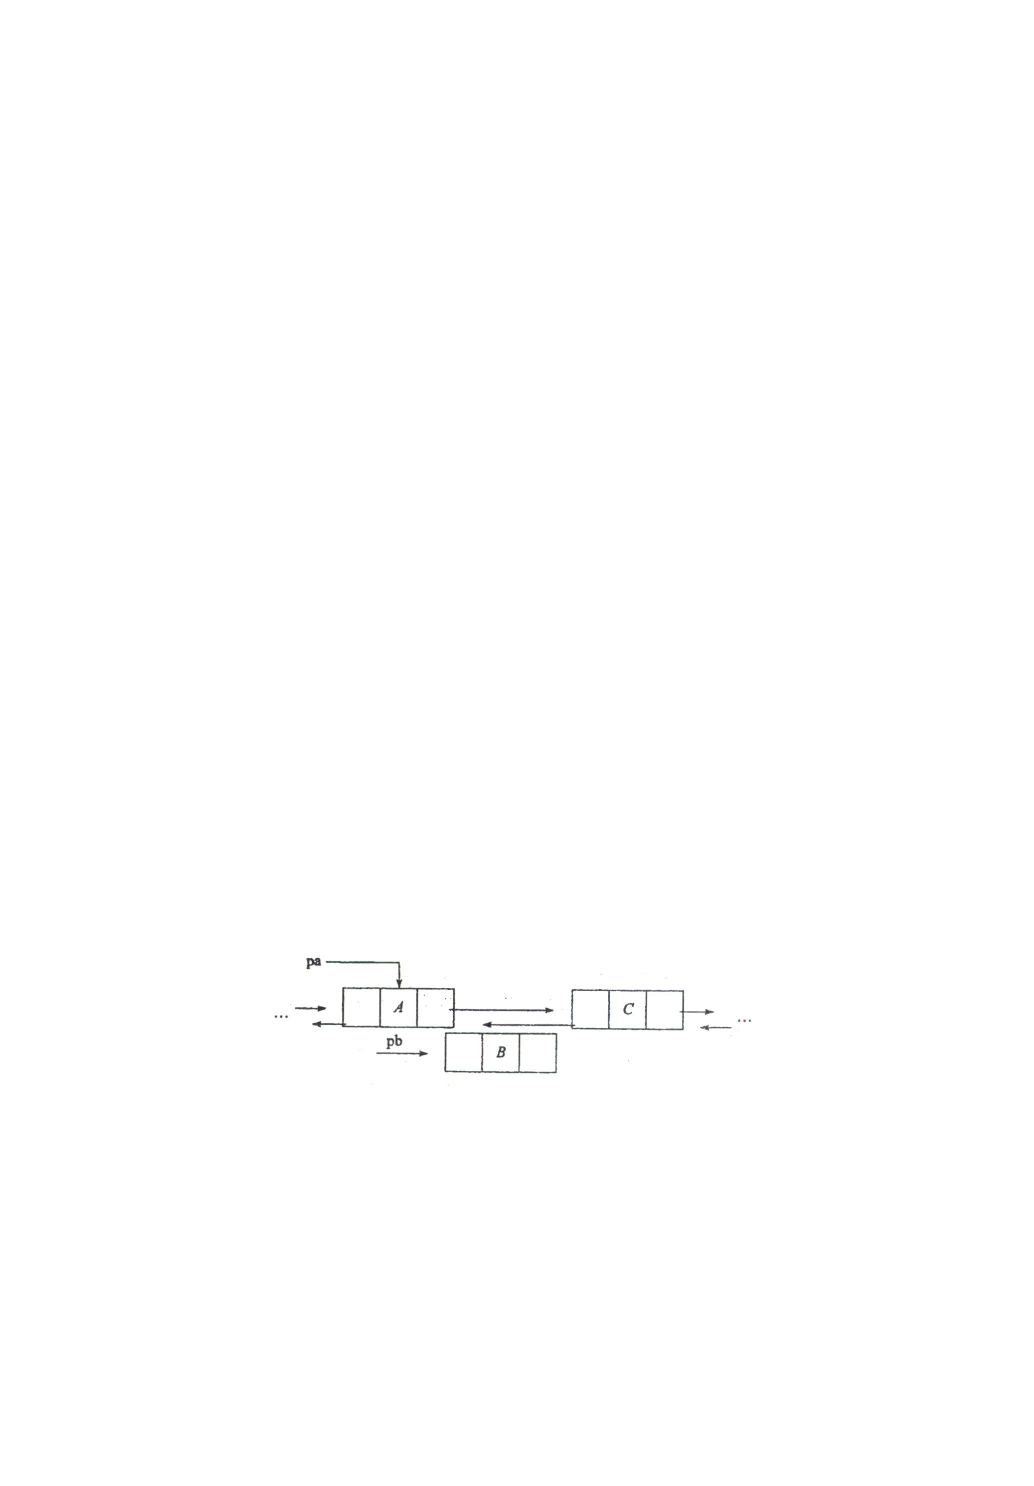
\includegraphics[width=0.5\textwidth]{../../figure/exercisePicPDF/chapter2/2-35.pdf}
        \caption{双向链表}
        \label{fig:linear_list_1}
    \end{figure}

    \begin{verbatim}
    (1) pb->next = pa->next;
    (2) pb->prior = pa;
    (3) pa->next = pb;
    (4) pa->next->prior = pb;
    \end{verbatim}

    A. (1)(2)(4)(3)

    B. (4)(3)(2)(1)  

    C. (3)(4)(1)(2)  

    D. (1)(4)(3)(2)  
    \item 对于顺序存储的线性表,访问结点和增加、删除结点的时间复杂度分别为( )。  
    【电子科技大学 2013 二、4(2 分);青岛大学 2000 五、1(2 分);烟台大学 2007 一、2(2 分)】  
   
    A. $O(n)$,$O(n)$ \quad B. $O(n)$,$O(1)$ \quad C. $O(1)$,$O(n)$ \quad D. $O(1)$,$O(1)$  

    \item 线性表的动态链表存储结构与顺序存储结构相比,优点是( )。  
    【暨南大学 2011 一、3(2 分)】  

    A. 所有的操作算法实现简单  

    B. 便于随机存取  

    C. 便于插入与删除  

    D. 便于节省存储器空间  

    \item 设线性表有 $2n$ 个元素,以下操作中,在单链表上实现要比在顺序表上实现效率更高的是( )。  
    【北京大学 2016 一、2(2 分)】  

    A. 删除指定元素  

    B. 在最后一个元素的后面插入一个新元素  

    C. 顺序输出前 $n$ 个元素  

    D. 交换第 $i$ 个元素和第 $2n-i-1$ 个元素的值($i=0, 1, \dots, n-1$)  

    \item 设单链表中指针 $p$ 指向结点 $a$,若要删除 $a$ 的直接后继结点,正确的操作是( )。  
    【烟台大学 2019 一、12(2 分)】  

    A. \texttt{p->next = p->next->next;}  

    B. \texttt{p = p->next;}  

    C. \texttt{p = p->next->next;}  

    D. \texttt{p->next = p;}  

    \item 根据教科书中线性表的实现方法,线性表中的元素必须是( )。  
    【北京理工大学 2007 一、1(1 分)】  

    A. 整数类型  

    B. 字符类型  

    C. 相同类型  

    D. 结构类型  

    \item 若经常需要按序号查找线性表中的数据元素,采用( )比较合适。  
    【北京理工大学 2007 一、2(1 分)】  

    A. 顺序存储结构  

    B. 链式存储结构  

    C. 静态链表  

    D. 链式存储结构或静态链表  

    \item 若链表中元素有序,下列叙述中正确的是( )。  
    【吉林大学 2016 一、1(2 分)】  

    A. 找第 $k$ 个大元素的时间复杂度为 $O(1)$  

    B. 查找一个元素是否属于链表的时间复杂度为 $O(n)$  

    C. 删除一个给定元素的时间复杂度为 $O(1)$  

    D. 插入一个给定元素的时间复杂度为 $O(n)$ 
\end{enumerate}

\chapter{栈与队列}
\begin{enumerate}
    \item 若栈 $S_1$ 中保存整数,栈 $S_2$ 中保存运算符,函数 $F()$ 依次执行下述各步操作:  
    
    1. 从 $S_1$ 中依次弹出两个操作数 $a$ 和 $b$;  

    2. 从 $S_2$ 中弹出一个运算符 $op$;  

    3. 执行相应的运算 $a \, op \, b$;

    4. 将运算结果压入 $S_1$ 中。  

    假定 $S_1$ 中的操作数依次是 $5, 8, 3, 2$($2$ 在栈顶),$S_2$ 中的运算符依次是 $*$,$-$,$+$($+$ 在栈顶)。调用 3 次 $F()$ 后,$S_1$ 栈顶保存的值是( )。  
    【2018 年全国试题 1(2 分)】  
    
    A. $-15$ \quad B. $15$ \quad C. $-20$ \quad D. $20$  

    \item 现有队列 $Q$ 与栈 $S$,初始时 $Q$ 中的元素依次是 $1, 2, 3, 4, 5, 6$($1$ 在队头),$S$ 为空。若仅允许下列 3 种操作:  
    
    1. $Q$ 出队并输出出队元素;  

    2. $Q$ 出队并将出队元素入栈;

    3. $S$ 出栈并输出出栈元素;  

    则不能得到的输出序列是( )。  
    【2018 年全国试题 2(2 分)】  

    A. $1, 2, 5, 6, 4, 3$  

    B. $2, 3, 4, 5, 6, 1$  

    C. $3, 4, 5, 6, 1, 2$  

    D. $6, 5, 4, 3, 2, 1$  

    \item 下列关于栈的叙述中,错误的是( )。  
    【2017 年全国试题 2(2 分)】  

    1. 采用非递归方式重写递归程序时必须使用栈;

    2. 函数调用时,系统要用栈保存必要的信息;  

    3. 只要确定了入栈次序,即可确定出栈次序;  

    4. 栈是一种受限的线性表,只允许在其两端进行操作。  

    A. 仅 1  

    B. 仅 1、3  

    C. 仅 1、3、4  

    D. 仅 1、2、4  


    \item 设有如下图所示的火车车轨,入口和出口之间有 $m$ 条轨道,列车的行进方向均为从左至右,列车可驶入任意一条轨道。现有编号为 $1 \sim 9$ 的 9 列列车,驶入的次序依次是 $8, 4, 2, 5, 3, 9, 1, 6, 7$。若期望驶出的次序依次为 $1 \sim 9$,则 $m$ 至少是( )。  
    【2016 年全国试题 3(2 分)】  

    \begin{figure}[h!]
        \centering
        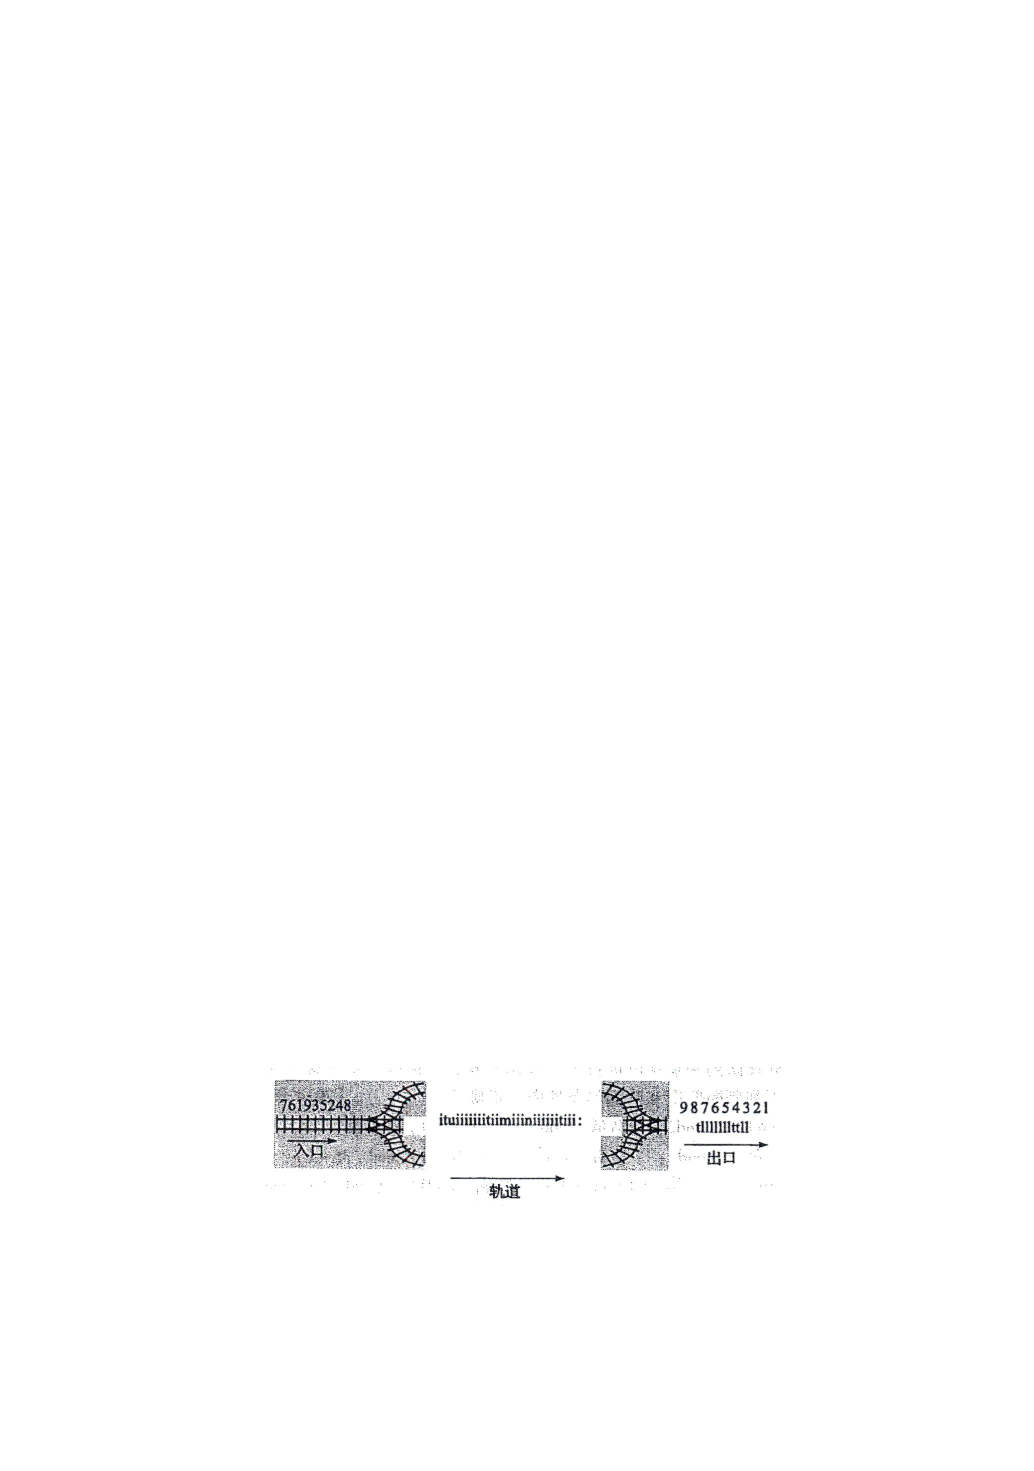
\includegraphics[width=0.5\textwidth]{../../figure/exercisePicPDF/chapter3/3-4.pdf}
        \caption{火车车轨}
        \label{fig:linear_list_2}
    \end{figure}
    A. 2 \quad B. 3 \quad C. 4 \quad D. 5  

    \item 为解决计算机主机与打印机之间的速度不匹配问题,通常设置一个打印数据缓冲区,主机将要输出的数据依次写入该缓冲区,而打印机则依次从该缓冲区中取出数据。该缓冲区的逻辑结构应该是( )。  
    【2009 年全国试题 1(2 分)】  
    
    A. 栈 \quad B. 队列 \quad C. 树 \quad D. 图  

    \item 设栈 $S$ 和队列 $Q$ 的初始状态均为空,
    元素 $a, b, c, d, e,f,g$ 依次进入栈 $S$。
    若每个元素出栈后立即进入队列 $Q$,且 5 个元素出队的顺序是 
    $b, d,c,f,e,a,g$,则栈 $S$ 的容量至少是( )。  
    【2009 年全国试题 2(2 分)】  
   
    A. 1 \quad B. 2 \quad C. 3 \quad D. 4  

    \item 若元素 $a, b, c, d, e,f$ 依次进栈,允许进栈、退栈操作交替进行,但不允许连续三次进行退栈操作,则不可能得到的出栈序列是( )。  
    【2010 年全国试题 1(2 分)】  

    A. $d, c, e, b,f, a$  

    B. $c, b, d, a, e,f$  

    C. $b,c, a, e,f, d $  

    D. $a,f,e,d,c,b$  

    \item 某队列允许在其两端进行入队操作,但仅允许在一端进行出队操作。若元素 $a, b, c, d, e$ 依次入此队列后再进行出队操作,则不可能得到的出队序列是( )。  
    【2010 年全国试题 2(2 分)】  

    A. $b, a, c, d, e$  

    B. $d, b, a, c, e$  

    C. $d,b,c,a,e$  

    D. $e, c, b, a, d$  

    \item 元素 $a, b, c, d, e$ 依次进入初始为空的栈中,若元素进栈后可停留、可出栈,直到所有元素都出栈,则在所有可能的出栈序列中,以元素 $d$ 开头的序列个数是( )。  
    【2011 年全国试题 2(2 分)】  

    A. 3 \quad B. 4 \quad C. 5 \quad D. 6  

    \item 已知循环队列存储在一维数组 $Q[0 \ldots m-1]$ 中,且队列非空时 \texttt{front} 和 \texttt{rear} 分别指向队头元素和队尾元素。若初始时队列为空,且要求第一个进入队列的元素存储在 $Q[0]$ 处,则初始时 \texttt{front} 和 \texttt{rear} 的值分别是( )。  
    【2011 年全国试题 3(2 分)】  

    A. 0, 0 \quad B. 0, $m-1$ \quad C. $m-1$, 0 \quad D. $m-1$, $m-1$  

    \item 已知操作符包括 $+$, $-$, $*$, $/$, $($ 和 $)$,
    将中缀表达式 $a+b-a*((c+d)/e-f)+g$ 转换为等价的后缀表达式时,用栈来存放暂时还不能确定运算次序的操作符。若栈初始时为空,则转换过程中同时保存在栈中的操作符的最大个数是( )。  
    【2012 年全国试题 2(2 分)】

    A. 5 \quad B. 7 \quad C. 8 \quad D. 11  

    \item 一个栈的入栈序列为 $1, 2, 3, \ldots, n$,其出栈序列是 $p_1, p_2, \ldots, p_n$。若 $p_1 = 3$,则 $p_2$ 可能取值的个数是( )。  
    【2013 年全国试题 2(2 分)】 

    A. $n-3$ \quad B. $n-2$ \quad C. $n-1$ \quad D. 无法确定  

    \item 假设栈初始为空,将中缀表达式 $a/b-(c*d-e*f)/g$ 转换为等价的后缀表达式的过程中,当扫描到 $/$ 时,栈中的元素依次是( )。  
    【2014 年全国试题 2(2 分)】  

    A. $+ ( * -$

    B.  $+ ( - *$

    C.  $/+(*-*$

    D.  $/+-*$

    \item 循环队列存放在一维数组 $Q[0 \ldots M-1]$ 中,\texttt{end1} 指向队头元素,\texttt{end2} 指向队尾元素的后一个位置。假设队列两端均可进行入队和出队操作,队列中最多能容纳 $M-1$ 个元素,初始时为空。下列判断队空和队满的条件中,正确的是( )。  
    【2014 年全国试题 3(2 分)】  

    A. 队空:\texttt{end1 == end2};队满:\texttt{end1 == (end2 + 1) mod M}  

    B. 队空:\texttt{end1 == end2};队满:\texttt{end2 == (end1 + 1) mod (M-1)}  

    C. 队空:\texttt{end2 == (end1 + 1) mod M};队满:\texttt{end1 == (end2 + 1) mod M}  

    D. 队空:\texttt{end1 == (end2 + 1) mod M};队满:\texttt{end2 == (end1 + 1) mod (M-1)}  

    \item 已知程序如下:
    \begin{verbatim}
    int s(int n) {
        return (n <= 0) ? 0 : s(n - 1) + n;
    }
    void main() {
        cout << s(1);
    }
    \end{verbatim}
    程序运行时使用栈来保存调用过程的信息,自栈底到栈顶保存的信息依次对应的是( )。  
    【2015 年全国试题 1(2 分)】  

    A. \texttt{main() -> s(1) -> s(0)}  

    B. \texttt{s(0) -> s(1) -> main()}  

    C. \texttt{main() -> s(0) -> s(1)}  

    D. \texttt{s(1) -> s(0) -> main()}  

    \item 栈的特点是( ),队列的特点是( ),栈和队列都是( )。若进栈序列为 $1, 2, 3, 4$,则( )不可能是一个出栈序列(不一定全部进栈后再出栈);若进队列的序列为 $1, 2, 3, 4$,则( )是一个出队列序列。  
    【北方交通大学 1999 一、1(5 分)】  
   
    A. 先进先出 \quad B. 后进先出 \quad C. 进优于出 \quad D. 出优于进  

    3️⃣:  

    A. 顺序存储的线性结构 

    B. 链式存储的线性结构  

    C. 限制存取点的线性结构  

    D. 限制存取点的非线性结构  

    出栈序列:  
    A. $3, 2, 1, 4$ \quad B. $3, 2, 4, 1$ \quad C. $3, 2, 1, 4$ \quad D. $4, 3, 2, 1$  

    \item 一个栈的输入序列为 $1, 2, 3, \ldots, n$,若输出序列的第一个元素是 $n$,则输出的第 $i$ ($1 < i < n$) 个元素是( )。  
    【电子科技大学 2012 一、4(2 分);中山大学 1999 一、9(1 分)】  

    A. 不确定  

    B. $n - i + 1$  

    C. $i$  

    D. $n-i$  

    \item 设栈的输入序列为 $1, 2, 3, \ldots, n$,输出序列为 $p_1, p_2, \ldots, p_n$。若 $p_1 = n$,则当 $n > i > 1$ 时,$p_i$ 为( )。若存在 $i > 1$ 使 $p_i = n$,则当 $i > j$ 时,$p_j$ 为( )。  
    【中国科学技术大学 1992 八、8(1 分)】  

    A. $p_i = n - i + 1$  

    B. $p_i$ 不确定  

    C. $p_j = n - j + 1$  

    \item 中缀表达式 $(A + B) * (C - D) / (E - F * G)$ 的后缀表达式是( )。  
   
    A. $A + B* C - D / E - F * G)$  

    B. $AB+CD-*EFG*-/$  

    C. $AB+C*D-E/F-G*$  

    D. $ABCDEFG+*-/-*$  
 

    \item 某表达式的前缀形式为 $+- ^ABCD/E/F + GH$,其等价的中缀表达式是( )。  
    【中国科学技术大学 1992 八、7(1 分)】  

    A. $A^B*C-D+E/F/G+H$  

    B. $A^B*(C-D) + E/F/G + H$  

    C. $A^B*C-D+E/(F/(G+H))$  

    D. $A^{B*(C-D)} +E/(F/(G+H))$  

    \item 表达式 $a*(b+c)-d$ 的后缀表达式是( )。  
    【南京理工大学 2001 一、2(1.5 分)】  

    A. $abcd *+-$  

    B. $abc+*d-$  

    C. $a b c * + d -$  

    D. $-+*abcd$  

    \item 与中缀表达式 $a * b + c / d - e$ 等价的前缀表达式是( )。  
    【华中科技大学 2006 一、5(2 分)】  

    A. $- + * a b / c d e$  

    B. $* + /-a b  c d  e$  

    C. $a b c d  e *+/-$  

    D. $+ * a b - / c d e$  

    \item 利用栈求表达式的值时,设立操作数栈 \texttt{OPND}。设 \texttt{OPND} 只有 $n$ 个元素。在下列表达式中,不发生上溢的是( )。  
    【四川大学 2005】  

    A. $a - b * (c - d)$  

    B. $(a - b) * c - d$  

    C. $(a - b * c) - d$  

    D. $(a - b) * (c - d)$  

    \item 有六个元素按 $6, 5, 4, 3, 2, 1$ 的顺序进栈,问下列哪一个不是合法的出栈序列( )。  
    【北方交通大学 2001 一、3(2 分)】  

    A. $5, 4, 3, 6, 1, 2$  

    B. $4, 5, 3, 1, 2, 6$  

    C. $3, 4, 6, 5, 2, 1$ 

    D. $2, 3, 4, 1, 5, 6$  

    \item 设栈的输入序列是 $1, 2, 3, 4$,则( )不可能是其出栈序列。  
    【中科院计算所 2000 一、10(2 分);烟台大学 2007 一、4(2 分)】  

    A. $1, 2, 4, 3$  

    B. $2, 1, 3, 4$  

    C. $1, 4, 3, 2$  

    D. $4, 3, 1, 2$  

    \item 四个元素 $1, 2, 3, 4$ 依次进栈,出栈次序不可能出现( )的情况。  
    【北京邮电大学 2005 一、1(2 分)】  

    A. $1, 2, 3, 4$  

    B. $4, 1, 3, 2$  

    C. $1, 4, 3, 2$  

    D. $4, 3, 2, 1$ 

    \item 如进栈序列为 $1, 2, 3, 4, 5$,可能得到的出栈序列为( )。  
    【上海交通大学 2005 四、1(2 分)】  

    A. $5, 4, 3, 2, 1$  

    B. $4, 5, 3, 2, 1$  

    C. $3, 4, 5, 2, 1$ 

    D. $2, 3, 4, 5, 1$  

    E. 都不可能  

    \item 一个栈的入栈序列为 $a, b, c, d, e$,则栈的不可能出栈序列是( )。  
    【中南大学 2005 一、2(2 分)】  

    A. $a, b, c, d, e$  

    B. $e, d, c, b, a$  

    C. $d, e, c, b, a$  

    D. $d, c, e, a,b$  

    \item 设 $n$ 个元素进栈序列是 $1, 2, 3, \ldots, n$,其输出序列是 $p_1, p_2, \ldots, p_n$。若 $p_1 = 3$,则 $p_2$ 的值为( )。  
    【武汉大学 2006】 

    A. 一定是 $2$  

    B. 一定是 $1$  

    C. 不可能是 $1$  

    D. 以上都不对  

    \item 某堆栈的输入序列为 $a, b, c, d$,下面的四个序列中,不可能是它的输出序列的是( )。  
    【北京航空航天大学 2000 一、3(2 分);北京邮电大学 1999 一、3(2 分)】  

    A. $a,c,b,d$  

    B. $b,c,d,a$  

    C. $c, d, b, a$  

    D. $d, c, a, b$  

    \item (多选) 若已知一个栈的入栈序列是 $1, 2, 3, 4$,其出栈序列为 $p_1, p_2, p_3, p_4$,则 $p_2, p_4$ 可能为( )。  
    【华中科技大学 2007 二、16(2 分)】  

    A. $2, 4$  

    B. $2, 1$  

    C. $4, 3$  

    D. $3, 4$  

    \item 输入序列为 $a, b, c$,可以变为 $c, b, a$ 时,经过的栈操作为( )。  
    【中山大学 1999 一、8(1 分)】  

    A. \texttt{push, pop, push, pop, push, pop}  

    B. \texttt{push, push, push, pop, pop, pop}  

    C. \texttt{push, push, pop, pop, push, pop} 

    D. \texttt{push, pop, push, push, pop, pop}  

    \item 依次读入数据元素序列 $a, b, c, d, e,f,g$,每进一个元素,机器可要求下一个元素进栈或弹出,如此进行,则栈空时弹出的元素构成的序列是以下哪些序列?  
    【哈尔滨工业大学 2000 七(8 分)】 

    A. $d,e,c,f,b,g,a$  

    B. $f,e,g,d,a,c,b$  

    C. $e, f,d, g,b, c, a$  

    D. $c, d, b,e,f,a,g$  

    \item 对于 4 个圆盘的汉诺塔,总的移动次数为( )。  
    【北京邮电大学 2005 一、3(2 分)】  

    A. $7$  

    B. $8$  

    C. $15$  

    D. $16$  

    \item 当字符序列作为右图输入时,输出长度为 3 且可用作 C 输出语言标识符的序列有( )。  
    【浙江大学 2004 二(5 分)】  

    \begin{figure}[h!]
        \centering
        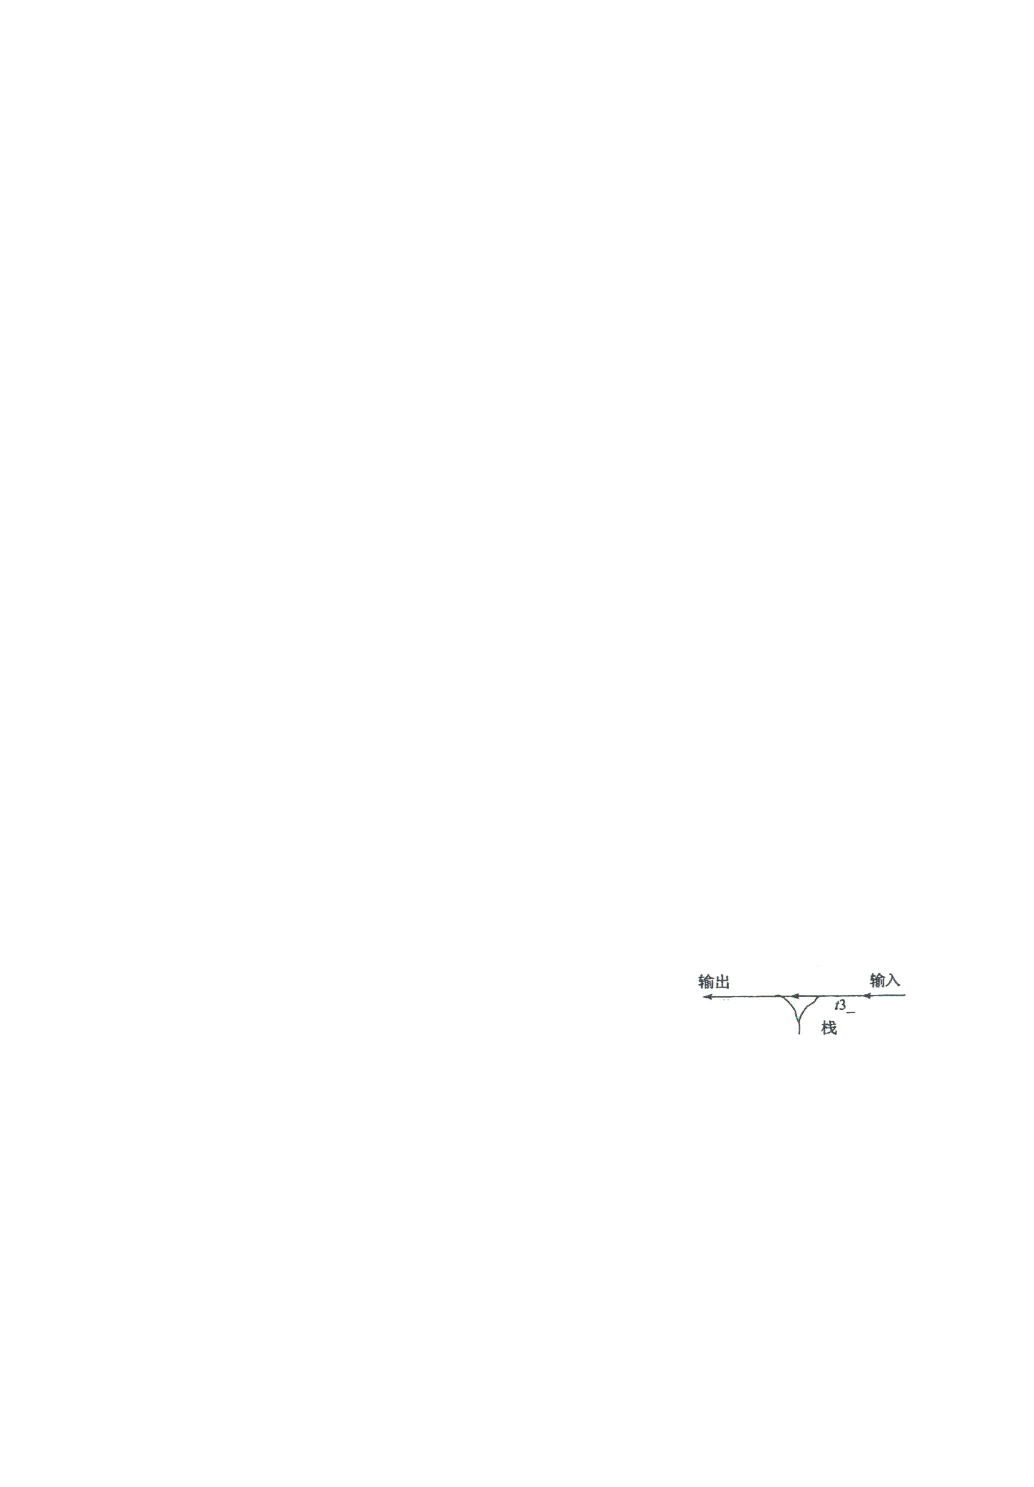
\includegraphics[width=0.5\textwidth]{../../figure/exercisePicPDF/chapter3/3-35.pdf}
        \caption{字符序列}
        \label{fig:linear_list_1}
    \end{figure}
    A. 4 个 \quad B. 5 个 \quad C. 3 个 \quad D. 6 个  

    \item 和顺序栈相比,链栈有一个比较明显的优势是( )。  
    【北京理工大学 2006 五、6(1 分)】

    A. 通常不会出现栈满的情况  

    B. 通常不会出现栈空的情况 

    C. 插入操作更容易实现  

    D. 删除操作更容易实现  

    \item 若一个栈以向量 $Y[1 \ldots n]$ 存储,初始栈顶指针 \texttt{top} 为 $n+1$,则下面进栈的正确操作是( )。  
    【南京理工大学 1998 一、13(2 分)】  

    A. \texttt{top = top + 1; V[top] = x;}  

    B. \texttt{V[top] = x; top = top + 1;}  

    C. \texttt{top = top - 1; V[top] = x;}  

    D. \texttt{V[top] = x; top = top - 1;}  

    \item 若栈采用顺序存储方式存储,现两栈共享空间 $Y[1 \ldots m]$,\texttt{top[i]} 表示第 $i$ 个栈($i=1, 2$)的栈顶,栈 1 的底在 $Y[1]$,栈 2 的底在 $Y[m]$,则栈满的条件是( )。  
    【南京理工大学 1999 一、14(1 分);江苏大学 2005 一、2(2 分)】  

    A. $| \texttt{top[2]} - \texttt{top[1]} | = 0$  

    B. $\texttt{top[1]} + 1 = \texttt{top[2]}$  

    C. $\texttt{top[1]} + \texttt{top[2]} = m$  

    D. $\texttt{top[1]} = \texttt{top[2]}$  

    \item 栈在( )中应用。  
    【中山大学 1998 二、3(2 分)】  

    A. 递归调用  

    B. 子程序调用  

    C. 表达式求值  

    D. A、B 和 C  

    \item 向一个栈顶指针为 $h$ 的带头结点的链栈中插入指针 $s$ 所指的结点时,应执行( )。  
    【北京理工大学 2005 才一、6(1 分)】  

    A. \texttt{h->next = s;}  
    
    B. \texttt{s->next = h;}  

    C. \texttt{s->next = h; h->next = s;}  

    D. \texttt{s->next = h->next; h->next = s;}  

    \item 一个递归算法必须包括( )。  
    【武汉大学 2000 二、2】  

    A. 递归部分  

    B. 终止条件和递归部分  

    C. 迭代部分  

    D. 终止条件和迭代部分  

    \item 假设某个循环队列采用数组 $C[0 \ldots 9]$ 表示,当前的队头指针 \texttt{front} 和队尾指针 \texttt{rear} 分别为 $4$ 和 $8$。首先执行两次入队操作,然后再执行两次出队操作,队头指针 \texttt{front} 和队尾指针 \texttt{rear} 应该分别变为( )。  
    【北京工业大学 2017 一、2(2 分)】  

    A. $5, 9$ \quad B. $6, 0$ \quad C. $0, 6$ \quad D. $6, 4$  

    \item 执行完下列语句段后,$f(1)$ 的值为( )。  
    【浙江大学 2000 一、6(3 分)】  

    \begin{verbatim}
    int f(int x) {
        return ((x > 0) ? x * f(x - 1) : 2);
    }
    int i;
    i = f(1);
    \end{verbatim}

    A. $2$ \quad B. $4$ \quad C. $8$ \quad D. 无限递归  

    \item 设计一个判别表达式中左、右括号是否配对出现的算法,采用( )数据结构最佳。  
    【西安电子科技大学 1996 一、6(2 分)】  

    A. 线性表的顺序存储结构  

    B. 队列  


    C. 线性表的链式存储结构  

    D. 栈  

    \item 递归过程或函数调用时,处理参数及返回地址要用一种称为( )的数据结构。  
    【福州大学 1998 一、1(2 分)】  

    A. 队列  

    B. 多维数组  

    C. 栈  

    D. 线性表  

    \item 允许对队列进行的操作有( )。  
    【华中科技大学 2004 一、2(1 分)】  

    A. 对队列中的元素排序  

    B. 取出最近进队的元素  

    C. 在队头元素之前插入元素  

    D. 删除队头元素  

    \item 若用单链表来表示队列,下面几种数据结构中,最合适的是( )。  
    【四川大学 2004】  

    A. 带尾指针的非循环链表  

    B. 带尾指针的循环链表  

    C. 带头指针的非循环链表  

    D. 带头指针的循环链表  

    \item 对于循环队列,( )。  
    【北京理工大学 2005 十一、7(1 分)】  

    A. 无法判断队列是否为空  

    B. 无法判断队列是否为满  

    C. 队列不可能满  

    D. 以上说法都不是  

    \item 循环队列 $Q[0 \ldots m-1]$ 存放其元素值,用 \texttt{front} 和 \texttt{rear} 分别表示队头和队尾;则当前队列中的元素数是( )。  
    【南京理工大学 2001 一、5(1.5 分)】  

    A. $(\texttt{rear} - \texttt{front} + m) \mod m$  

    B. $\texttt{rear} - \texttt{front} + 1$  

    C. $\texttt{rear} - \texttt{front} - 1$  

    D. $\texttt{rear} - \texttt{front}$  

    \item 若循环队列使用 C 数组 $Q[m]$ 存放其数据元素,已知头指针 \texttt{front} 指向队首元素,尾指针 \texttt{rear} 指向队尾元素后的空单元,则当前队列中的元素个数为( )。  
    【华中科技大学 2007 一、3(2 分)】 

    A. $(\texttt{rear} - \texttt{front} + m) \mod m$  

    B. $\texttt{rear} - \texttt{front} + 1$  

    C. $\texttt{rear} - \texttt{front}$  

    D. $\texttt{rear} - \texttt{front} - 1$  

    \item 设顺序队列的容量为 \texttt{MaxSize},其头指针为 \texttt{front},尾指针为 \texttt{rear},空队列的条件为( )。  
    【电子科技大学 2008 一、4(2 分)】  

    A. $\texttt{front} = \texttt{rear}$  

    B. $\texttt{front} = \texttt{MaxSize}$  

    C. $\texttt{front} + 1 = \texttt{rear}$  

    D. $\texttt{rear} = 0$  

    \item 循环队列存储在数组 $Q[0 \ldots m]$ 中,则入队时的操作为( )。  
    【中山大学 1999 一、6(1 分)】  

    A. $\texttt{rear} = \texttt{rear} + 1$  

    B. $\texttt{rear} = (\texttt{rear} + 1) \mod (m - 1)$  

    C. $\texttt{rear} = (\texttt{rear} + 1) \mod m$  

    D. $\texttt{rear} = (\texttt{rear} + 1) \mod (m + 1)$  

    \item 若用一个大小为 6 的数组来实现循环队列,且当前 \texttt{rear} 和 \texttt{front} 的值分别为 $0$ 和 $3$,那么从队列中删除一个元素再加入两个元素后,\texttt{rear} 和 \texttt{front} 的值分别为多少?( )  
    【北京大学 2016 一、4(2 分)】  

    A. $1$ 和 $5$ \quad B. $2$ 和 $4$ \quad C. $4$ 和 $2$ \quad D. $5$ 和 $1$  

    \item 若以 $1, 2, 3, 4$ 作为双端队列的输入序列,则既不能由输入受限的双端队列得到,也不能由输出受限的双端队列得到的输出序列是( )。  
    【西安电子科技大学 1996 一、5(2 分);烟台大学 2007 一、5(2 分)】  

    A. $1, 2, 3, 4$  

    B. $4, 1, 3, 2$  

    C. $4, 2, 3, 1$  

    D. $4, 2, 1, 3$  

    \item 下列关于栈的叙述中,正确的是( )。  
    【华北电力大学 2018 一、7】  

    A. 栈底元素一定是最后入栈的元素  

    B. 栈操作遵循先进后出的原则  

    C. 栈顶元素一定是最先入栈的元素  

    D. 以上三种说法都不对  

    \item 最大容量为 $m$ 的循环队列,队尾指针是 \texttt{rear},队头指针是 \texttt{front},则队空的条件是( )。  
    【南京理工大学 1999 一、16(2 分)】  

    A. $(\texttt{rear} + 1) \mod m = \texttt{front}$  

    B. $\texttt{rear} = \texttt{front}$  

    C. $\texttt{rear} + 1 = \texttt{front}$  

    D. $(\texttt{rear} - 1) \mod m = \texttt{front}$  

    \item 栈和队列的共同点是( )。  
    【大连理工大学 2004 一、1(2 分)】  

    A. 都是先进后出  

    B. 都是后进先出  

    C. 只允许在端点处插入和删除元素  

    D. 没有共同点  

    \item 将递归算法转变成对应的非递归算法时,需要使用( )保存中间结果。  
    【华中科技大学 2007 一、15(2 分)】  

    A. 栈 \quad B. 队列 \quad C. 二叉树 \quad D. 单链表  

    \item 队列的“先进先出”特性是指( )。  
    【武汉理工大学 2004 一、4(3 分)】  

    A. 最后插入队列中的元素总是最后被删除  

    B. 当同时进行插入、删除操作时,总是插入操作优先  

    C. 每当有删除操作时,总要先做一次插入操作  

    D. 每次从队列中删除的总是最早插入的元素  

    \item 设栈 $S$ 和队列 $Q$ 的初始状态为空,元素 $a, b, c, d, e, f$ 依次通过栈 $S$,一个元素出栈后即进队列 $Q$,
    若 6 个元素出队的序列是 $b, d, c, f, e, a$,则栈 $S$ 的容量至少应为( )。  
    【南京理工大学 2000 一、6(1.5 分);哈尔滨工业大学 2004 二、3(1 分)】

    A. $6$ \quad B. $4$ \quad C. $3$ \quad D. $2$  

    \item 设有 5 个元素 $1, 2, 3, 4, 5$ 顺序进栈,下列几个选项中,不可能出现的出栈序列是( )。  
    【北京大学 2015 一、3(1.5 分)】  

    A. $1,2,3,4,5$  

    B. $4,5,3,2,1$ 

    C. $1,3,5,2,4$  

    D. $3,2,1,4,5$  

    \item 实现时需使用队列的运算是( )。  
    【电子科技大学 2005 一、9(1 分)】  

    A. 递归过程  

    B. 二叉树的中序遍历  

    C. 图的深度优先搜索 

    D. 二叉树的层次遍历  

    \item 下列更合适表示队列的链表结构是( )。  
    【北京理工大学 2006 九、6(1 分)】  

    A. 单向链表  

    B. 单向循环链表  

    C. 双向链表  

    D. 双向循环链表  

    \item 队列操作的原则是( )。  
    【暨南大学 2010 一、2(2 分)】  

    A. 先进先出  

    B. 后进先出  

    C. 只能进行插入  

    D. 只能进行删除  

    \item 执行( )操作时,需要使用队列作辅助存储空间。  
    【华中科技大学 2006 一、5(2 分)】  

    A. 查找哈希(Hash)表  

    B. 广度优先搜索网  

    C. 先序(根)遍历二叉树  

    D. 深度优先搜索网  

    \item 在下列栈的基本操作中,( )初始条件不要求栈S已存在。  
    【北京理工大学 2007 一、3(1 分)】  

    A. \texttt{InitStack(\&S)}  

    B. \texttt{DestoryStack(\&S)}  

    C. \texttt{ClearStack(\&S)}  

    D. \texttt{StackEmpty(S)}  

    \item 在算符优先级中,算符 “$+$” 和 “$($” 的优先关系是( )。  
    【北京理工大学 2007 一、5(1 分)】  

    A. $+$ > $($  

    B. $+$ < $($  

    C. $+$ = $($  

    D. 取决于它们出现的位置  

    \item 在带头结点的链队列中,头指针指向链表的( )。  
    【北京理工大学 2007 一、4(1 分)】  

    A. 最后一个元素结点  

    B. 第一个元素结点  

    C. 头结点  

    D. 都不是  

    \item 采用顺序存储结构的栈 $S$ 和队列 $Q$ 的初始状态均为空,元素 $a, b, c, d, e, f$ 依次进入队列 $Q$,
    $Q$ 中的每一个元素出队后立刻进入栈 $S$,如果 6 个元素的出栈序列是 $b,c,d,f,e,a$,则栈 $S$ 的容量最少是( )。  
    【北京工业大学 2018 一、5(2 分)】  

    A. $2$ \quad B. $3$ \quad C. $4$ \quad D. $5$  

    \item 设输入序列为 $1, 2, 3, 4, 5$,下列选项中,不可能是其出栈序列的是( )。  
    【吉林大学 2016 一、3(2 分)】  

    A. $2, 4, 3, 5, 1$  

    B. $3, 4,1,5,2$  

    C. $3, 2, 4, 1, 5$  

    D. $4,1,3,2,5$  

    \item 已知一个算术表达式的中缀形式为 $A + B * C - D / E$,后缀形式为 $A B C * + D E / -$,则其前缀形式为( )。  
    【北京大学 2015 一、4(1.5 分)】  

    A. $-A+B*C/DE$  

    B. $-A+B*CD/E$  

    C. $-+*ABC/DE$  

    D. $-+A*BC/DE$  

    \item 有 5 个元素,其入栈次序为 $a, b, c, d, e$,在各种可能的出栈次序中,以 $c$ 最先出栈的次序不包括( )。  
    【北京大学 2016 一、3(2 分)】  

    A. $c, d, e, b, a$  

    B. $c, d, b, e, a$  

    C. $c, d, b, a, e$  

    D. $c, d, a, e, b$  
\end{enumerate}

\chapter{串}
\begin{enumerate}

    \item 设主串 $S = \texttt{"abaabaabcabaabc"}$,模式串 $P = \texttt{"abaabc"}$,采用 KMP 算法进行模式匹配,到匹配成功时为止,在匹配过程中进行的单个字符间的比较次数是( )。  
    【2019 年全国试题 9(2 分)】

    A. 9 \quad B. 10 \quad C. 12 \quad D. 15  

    \item 已知字符串 $S = \texttt{"abaabaabacacaabaabcc"}$,模式串 $P = \texttt{"abaabc"}$,采用 KMP 算法进行匹配,第一次出现“失配”($S[i] \neq P[j]$)时,$i=5$ 且 $j=5$,则下次开始匹配时,$i$ 和 $j$ 的值分别是( )。  
    【2015 年全国试题 8(2 分)】  

    A. $i=1, j=0$ \quad B. $i=5, j=0$ \quad C. $i=5, j=2$ \quad D. $i=6, j=2$  

    \item 下面关于串的叙述中,哪一个是不正确的( )。  
    【北方交通大学 2001 一、5(2 分);江苏大学 2005 一、6(2 分)】  

    A. 串是字符的有限序列  

    B. 空串是由空格构成的串  

    C. 模式匹配是串的一种重要运算 

    D. 串既可以采用顺序存储,也可以采用链式存储  

    \item 若串 $S_1 = \texttt{"ABCDEFG"}$,$S_2 = \texttt{"9898"}$,$S_3 = \texttt{"\#\#\#"}$,$S_4 = \texttt{"012345"}$,
    执行  
    \texttt{concat(replace(S1, substr(S1, length(S2), length(S3)), S3), substr(S4, index(S2, '8'), length(S2)))}  
    其结果为( )。  
    【北方交通大学 1999 一、5(2 分)】  

    A. \texttt{"ABC\#\#\#{G0123}"} \quad B. \texttt{"ABCD\#\#\#{2345}"}  

    C. \texttt{"ABC\#\#\#{G2345}"} \quad D. \texttt{"ABC\#\#\#{2345}"}  

    E. \texttt{"ABC\#\#\#{G1234}"} \quad F. \texttt{"ABCD\#\#\#{1234}"}  

    G. \texttt{"ABC\#\#{01234}"}
    \item 设有两个串 $S_1$ 和 $S_2$,求 $S_2$ 在 $S_1$ 中首次出现的位置的运算称作( )。  
    【中南大学 2005 一、3(2 分)】  

    A. 求子串 \quad B. 判断是否相等 \quad C. 模式匹配 \quad D. 连接  

    \item 已知串 $S = \texttt{"aaab"}$,其 Next 数组值为( )。  
    【西安电子科技大学 1996 一、7(2 分)】 

    A. $(0, 1, 2, 3)$ \quad B. $(1, 1, 2, 3)$ \quad C. $(1, 2, 3, 1)$ \quad D. $(1, 2, 1, 1)$  

    \item 串 \texttt{"ababaaababaa"} 的 Next 数组为( )。  
    【中山大学 1999 一、7;江苏大学 2006 一、1(2 分)】  

    A. $(0, 1, 2, 3, 4, 5, 6, 7, 8,9,9,9)$  

    B. $(0, 1, 2, 1, 2, 1, 1, 1, 1,2,1,2)$  

    C. $(0, 1, 1, 2, 3, 4, 2, 2, 3,4,5,6)$  

    D. $(0, 1, 2, 3, 0, 1, 2, 3, 2,2,3,4)$  

    \item 字符串 \texttt{"ababaabab"} 的 NextVal 数组为( )。  
    【北京邮电大学 1999 一、1(2 分);烟台大学 2007 一、8(2 分)】  

    A. $(0, 1, 0, 1, 0, 4, 1, 0, 1)$  

    B. $(0, 1, 0, 1, 0, 2, 1, 0, 1)$  

    C. $(0, 1, 0, 1, 0, 0, 0, 1, 1)$  

    D. $(0, 1, 0, 1, 0, 1, 0, 1, 1)$  

    \item 模式串 $P = \texttt{"abcaabbcabcaabdab"}$,该模式串的 Next 数组的值为( ),NextVal 数组的值为( )。  
    
    A. 01112211123456712 

    B. 01112121123456112 

    C. 01110013101100701 

    D. 01112231123456712 

    E. 01100111011001701 

    F. 01102131011021701  

       \item 若串 $S = \texttt{"myself"}$,则其子串的数目是( )。  
       【北京理工大学 2007 一、6(1 分)】  

       A. 20 \quad B. 21 \quad C. 22 \quad D. 23  
   
       \item 若串 $S = \texttt{"software"}$,则其子串的数目是( )。  
       【西安电子科技大学 2001 应用一、2(2 分)】  

       A. 8 \quad B. 37 \quad C. 36 \quad D. 9  
   
       \item 设 $S$ 是一个长度为 $m$ 的字符串,其中的字符各不相同,则 $S$ 中互异的非平凡子串(非空且不同于 $S$ 本身)的个数为( )。  
       【中科院计算所 1997;烟台大学 2007 一、7(2 分)】  

       A. $2m - 1$  

       B. $m^2$  

       C. $\frac{m^2}{2} + m/2$  

       D. $\frac{m^2}{2} + m/2 - 1$  

       E. $\frac{m^2}{2} - m/2 - 1$  

       F. 其他情况  
   
       \item 串是一种特殊的线性表,其特殊性体现在( )。  
       【暨南大学 2010 一、11(2 分)】  

       A. 可以顺序存储  

       B. 数据元素是一个字符  

       C. 可以链接存储  

       D. 数据元素可以是多个字符  
   
       \item 在下列表述中,( )是错误的。  
       【华中科技大学 2006 二、2(2 分)】  


       A. 含有一个或多个空格字符的串称为空格串  

       B. 对 $n$ ($n > 0$) 个顶点的网,求出权最小的 $n-1$ 条边便可构成其最小生成树  

       C. 选择排序算法是不稳定的  

       D. 平衡二叉树的左右子树的结点数之差的绝对值不超过 1  
\end{enumerate}

\chapter{数组和广义表}


\begin{enumerate}
    \item 设有一个 $12 \times 12$ 的对称矩阵 $M$,将其上三角部分的元素 $m_{ij}$ ($1 \leq i \leq j \leq 12$) 按行优先存入 C 语言的一维数组 $N$ 中,
    元素 $m_{6,6}$ 在 $N$ 中的下标是( )。  
    【2018 年全国试题 3(2 分)】  

    A. 50 \quad B. 51 \quad C. 55 \quad D. 66  

    \item 适用于压缩存储稀疏矩阵的两种存储结构是( )。  
    【2017 年全国试题 3(2 分)】  

    A. 三元组表和十字链表  

    B. 三元组表和邻接矩阵  

    C. 十字链表和二叉链表 

    D. 邻接矩阵和十字链表  

    \item 有一个 100 阶的三对角矩阵 $M$,其元素 $m_{ij}$ ($1 \leq i, j \leq 100$) 按行优先次序压缩存入下标从 0 开始的一维数组 $N$ 中。元素 $m_{30,30}$ 在 $N$ 中的下标是( )。  
    【2016 年全国试题 4(2 分)】  

    A. 86 \quad B. 87 \quad C. 88 \quad D. 89  

    \item 数组 $A[0..5, 0..6]$ 的每个元素占 5 个字节,将其按列优先次序存储在起始地址为 1000 的内存单元中,则元素 $A[5,5]$ 的地址是( )。  
    【南京理工大学 2001 一、13(1.5 分)】 

    A. 1175 \quad B. 1180 \quad C. 1205 \quad D. 1210  

    \item 设 7 行 6 列的数组 $A$ 以列序为主序顺序存储,基地址为 1024,每个元素占 2 个存储单元,第 4 行第 5 列的元素(假定无第 0 行第 0 列)的存储地址是( )。  
    【华中科技大学 2006 一、3(2 分)】 

    A. 1068 \quad B. 1086 \quad C. 1084 \quad D. 1066  

    \item 若 6 行 5 列的数组以列序为主序顺序存储,基地址为 1000,每个元素占 2 个存储单元,则第 3 行第 4 列的元素(假定无第 0 行第 0 列)的地址是( )。  
    【华中科技大学 2004 一、4(1 分)】 

    A. 1040 \quad B. 1042 \quad C. 1026 \quad D. 备选答案 A、B、C 都不对  

    \item 二维数组 $A$ 的元素都是 6 个字符组成的串,行下标 $i$ 的范围从 0 到 8,列下标 $j$ 的范围从 1 到 10。从供选择的答案中选出应填入下列关于数组存储叙述中( )内的正确答案。  
    【山东工业大学 2000 三、1(4 分);山东大学 1998 三、1(4 分)】  

    (1) 存放 $A$ 至少需要( )个字节;  

    (2) $A$ 的第 8 列和第 5 行共占( )个字节;  

    (3) 若 $A$ 按行存放,元素 $A[8,5]$ 的起始地址与 $A$ 按列存放时的元素( )的起始地址一致。  

    供选择的答案:  

    (1) A. 90 \quad B. 180 \quad C. 240 \quad D. 270 \quad E. 540  

    (2) A. 108 \quad B. 114 \quad C. 54 \quad D. 60 \quad E. 150  

    (3) A. $A[8,5]$ \quad B. $A[3,10]$ \quad C. $A[5,8]$ \quad D. $A[0,9]$  

    \item 设二维数组 $A[1..m, 1..n]$(即 $n$ 行 $m$ 列)按行存储在数组 $B[1..n \cdot m]$ 中,则二维数组元素 $A[i,j]$ 在一维数组 $B$ 中的下标为( )。  
    【南京理工大学 1998 一、2(2 分)】  

    A. $(i-1) \cdot n + j$  

    B. $(i-1) \cdot n + j - 1$  

    C. $i \cdot (j - 1)$  

    D. $j \cdot m + i - 1$  

    \item 将一个 $A[1..100, 1..100]$ 的三对角矩阵按行优先存入一维数组 $B[1..298]$ 中,$A[66,65]$ 在数组中的位置是( )。  
    【北京邮电大学 1998 二、5(2 分)】  

    A. 198 \quad B. 195 \quad C. 197  

    \item 数组通常具有的两种基本操作是( )。  
    【中南大学 2005 一、10(2 分)】  

    A. 查找和修改 \quad B. 查找和索引 \quad C. 索引和修改 \quad D. 建立和删除  

    \item 对矩阵压缩存储是为了( )。  
    【中南大学 2005 一、9(2 分)】  

    A. 方便运算 \quad B. 方便存储 \quad C. 提高运算速度 \quad D. 减少存储空间  

    \item 稀疏矩阵一般的压缩存储方法有两种,即( )。  
    【华南理工大学 2005 一、1(2 分);暨南大学 2010 一、12(2 分);江苏大学 2005 一、9(2 分)】  

    A. 二维数组和三维数组  

    B. 三元组和散列  

    C. 三元组和十字链表  

    D. 散列和十字链表  

    \item 假设包含 $t$ 个非零元素的稀疏矩阵 $A$ 含有 $m$ 行 $n$ 列,并采用三元组顺序表压缩存储,其快速转置算法的时间复杂度为( )。  
    【北京工业大学 2013 一、4(2 分)】

    A. $O(m+t)$ \quad B. $O(n+t)$ \quad C. $O(m+n)$ \quad D. $O(m*n)$  

    \item 稀疏矩阵的三元组存储方法( )。  
    【华南理工大学 2006 一、4(2 分)】  

    A. 实现转置运算很简单,只需将每个三元组的行标和列标交换  

    B. 是一种链式存储方法  

    C. 对矩阵的非零元个数和位置在操作过程中变化不大时较有效  

    D. 比十字链表法更高效  

    \item 在稀疏矩阵的快速转置算法中,\texttt{num[col]} 表示源矩阵 $N$ 中( )。  
    【北京理工大学 2007 一、7(1 分)】  

    A. 第 \texttt{col} 行中非零元的个数  

    B. 第 \texttt{col} 行中零元的个数  

    C. 第 \texttt{col} 列中非零元的个数  

    D. 第 \texttt{col} 列中零元的个数  

    \item 设有一个 $n \times n$ 的对称矩阵 $A$,将其下三角部分按行存放在一个一维数组 $B$ 中,$A[0][0]$ 存放于 $B[0]$ 中,则第 $i$ 行的对角元素 $A[i][i]$ 存放于 $B$ 中的位置是( )。  
    【哈尔滨工业大学 2005(2 分)】  

    A. $(i+3) \cdot i / 2$ \quad B. $(i+1) \cdot i / 2$ \quad C. $(2n-i+1) \cdot i / 2$ \quad D. $(2n-i-1) \cdot i / 2$  

    \item 对 $n$ 阶对称矩阵 $A$ 以行序为主序方式将其下三角形的元素(包括主对角线上所有元素)依次存放于一维数组 $B[1..n(n+1)/2]$ 中,则在 $B$ 中确定 $A[i][j]$ ($i \geq j$) 的位置关系为( )。  
    【北京航空航天大学 2000 一、2(2 分);烟台大学 2007 一、9(2 分)】  

    A. $i \cdot (i-1)/2 + j$  

    B. $j \cdot (j-1)/2 + i$  

    C. $i \cdot (i+1)/2 + j$  

    D. $j \cdot (j+1)/2 + i$  

    \item 设 $A$ 是 $n \times n$ 的对称矩阵,将 $A$ 的对角线及对角线上方的元素以列为主的次序存放在一维数组 $B[1..n(n+1)/2]$ 中,上述任一元素 $m_{ij}$ ($1 \leq i, j \leq n$ 且 $i \leq j$) 在 $B$ 中的位置为( )。  
    【南京理工大学 1999 一、9(2 分);江苏大学 2006 一、1(2 分)】 

    A. $j \cdot (j-1)/2 + i$  

    B. $i \cdot (i-1)/2 + j$  

    C. $j \cdot (j-1)/2 + i - 1$  

    D. $i \cdot (i-1)/2 + j - 1$  

    \item 对 $n$ 阶对称矩阵作压缩存储时,需要表长为( )的顺序表。  
    【华中科技大学 2006 一、7(2 分)】  

    A. $n/2$ \quad B. $n^2/2$ \quad C. $n(n+1)/2$ \quad D. $n(n-1)/2$  

    \item 有一个 $100 \times 90$ 的稀疏矩阵,非零元素有 10 个,设每个整型数占 2 字节,则用三元组表示该矩阵时,所需的字节数是( )。  
    【南京理工大学 1999 二、8(2 分)】  

    A. 60 \quad B. 66 \quad C. 18,000 \quad D. 33 

    \item 数组 $A[0..4, -1..-3, 5..7]$ 中含有的元素个数是( )。  
    【中山大学 1998 二、5(2 分)】  

    A. 55 \quad B. 45 \quad C. 36 \quad D. 16  

    \item 用数组r存储静态链表,结点的 \texttt{next} 域指向后继,工作指针 $J$ 指向链中结点,使 $J$ 沿链移动的操作为( )。  
    【南京理工大学 2001 一、16(1.5 分)】  

    A. \texttt{J = r[J].next}  

    B. \texttt{J = J + 1}  

    C. \texttt{J = J->next}  

    D. \texttt{J = r[J]->next}  

    \item 一个非空广义表的表尾是( )。  
    【北京交通大学 2004 一、2(2 分)】  

    A. 不能是子表  

    B. 只能是子表  

    C. 只能是原子  

    D. 是原子或子表  

    \item 广义表 $(((a)), ((b, (c)), (d, (e, f))), ())$ 的深度是( )。  
    【华中科技大学 2007 一、7(2 分)】  

    A. 2 \quad B. 3 \quad C. 4 \quad D. 5  

    \item 广义表 $(a, ((b, (c, d, (e, f))), g))$ 的深度为( )。  
    【北京邮电大学 2005 一、4(2 分)】  

    A. 3 \quad B. 4 \quad C. 5 \quad D. 6  

    \item 广义表 $((a, b), c, (d, (e)))$ 的表尾是( )。  
    【华中科技大学 2006 一、4(2 分)】  

    A. $(d, (e))$  

    B. $((d, (e)))$  

    C. $e$  

    D. $(c, (d, (e)))$  

    \item 已知广义表 $(()$, $(a)$, $(b, c, (d)$, $((d, f))))$,则以下说法正确的是( )。  
    【华南理工大学 2006 一、7(2 分)】  

    A. 表长为 3,表头为空表,表尾为 $((a), (b, c, (d), ((d, f))))$  

    B. 表长为 3,表头为空表,表尾为 $(b, c, (d), ((d, f)))$  

    C. 表长为 4,表头为空表,表尾为 $((d, f))$  

    D. 表长为 3,表头为 $(()$,表尾为 $((a), (b, c, (d), ((d, f))))$  

    \item 已知广义表 $LS = ((a, b, c), (d, e, f))$,运用 \texttt{head} 和 \texttt{tail} 函数取出 $LS$ 中原子 $e$ 的运算是( )。  
    【西安电子科技大学 2001 应用一、3(2 分)】

    A. \texttt{head(tail(LS))}  

    B. \texttt{tail(head(LS))}  

    C. \texttt{head(tail(head(tail(LS))))}  

    D. \texttt{head(tail(tail(head(LS))))}  

    \item 已知广义表 $A = (a, b, (c, d), (e, (f, g)))$,则下面式子 \texttt{Head(Tail(Head(Tail(Tail(A))))) } 的值为( )。  
    【北京邮电大学 1999 一、2(2 分);烟台大学 2007 一、10(2 分)】

    A. $(g)$ \quad B. $(d)$ \quad C. $c$ \quad D. $d$  

    \item 设广义表 $Z = (a, b, ())$,则 \texttt{GetTail(GetTail(Z))} 的结果是( )。  
    【北京理工大学 2006 九、8(1 分)】  

    A. $(())$ \quad B. $()$ \quad C. $(b, ())$ \quad D. 都不是  

    \item 广义表 $A = (a, b, c, (d, (e, f)))$,则下面式子 \texttt{Head(Tail(Tail(Tail(A))))} 的值为( )。  
    【华南理工大学 2005 一、1(2 分)】  

    A. $(d, (e, f))$ \quad B. $d$ \quad C. $f$ \quad D. $(e, f)$  

    \item 某字符串满足 \texttt{concat(head(s), head(tail(tail(s)))) = "ac"}(\texttt{head} 和 \texttt{tail} 的定义同广义表),则 $s$ 是( )。  
    【中国科学技术大学 1992 八、6(1 分)】  

    A. \texttt{"aabc"} \quad B. \texttt{"acba"} \quad C. \texttt{"accc"} \quad D. \texttt{"acac"}  

    \item 广义表 $(a, (b, c), d, e)$ 的表头为( )。  
    【中山大学 1998 二、6(2 分)】  

    A. $a$  

    B. $a, (b, c)$  

    C. $(a, (b, c))$  

    D. $(a)$  

    \item 已知 \texttt{Head(Tail([Head(S), Head(Tail(Tail(S)))])) = [a]},广义表 $S$ 满足上式,则 $S$ 为( )。  
    (其中,方括号表示广义表,圆括号表示函数,如 $[a, b]$ 表示由 $a, b$ 构成的广义表,而 \texttt{Head()} 表示取广义表的头部)  

    A. [[a, b], b, a]  

    B. [[b, a], [a], [b]]  

    C. [[a], [a, b], [b]]  

    D. [b, [a], [a, b]]  

    E. [[a],[b], [b, a]]  

    F. [[b],[b,a], [a]]


    \item 广义表 $(( ))$ 的表头是( ),表尾是( )。  
    【电子科技大学 2003 一、4(2 分)】  

    A. $()$  

    B. $NIL$

    C. $(())$ 

    D. $((()))$  

    \item 将线性表的数据元素进行扩充,允许带结构的线性表是( )。  
    【电子科技大学 2001 一、8(1 分)】  

    A. 串  

    B. 树  

    C. 广义表  

    D. 栈  

    \item 下面说法不正确的是( )。  
    【南京理工大学 2001 一、3(1.5 分);江苏大学 2006 一、1(2 分)】 

    A. 广义表的表头总是一个广义表  

    B. 广义表的表尾总是一个广义表  


    C. 广义表难以用顺序存储结构  

    D. 广义表可以是一个多层次的结构  

    \item 下面说法不正确的是( )。  
    【电子科技大学 2008 一、5(1 分)】  

    A. 广义表的表尾总是一个广义表  

    B. 广义表难以用顺序存储结构  

    C. 广义表的表头总是一个广义表  

    D. 广义表可以是一个递归结构  

    \item 广义表 $S$ 的表头为 $(a, (b, c))$,表尾为 $((d, e), f,(g, h))$,则 $S$ 是( )。  
    【北京工业大学 2018 一、9(2 分)】  

    A. $(a, ((b, c)), ((d, e),f, (g, h)))$  

    B. $((a, (b, c)), (d, e), f, (g, h))$  

    C. $((a, (b, c)), ((d, e), f, (g, h)))$  

    D. $(a, (b, c), (d, e), f, (g, h))$  

    \item 按行优先存储的四维数组 $A = \texttt{array[1..10, 1..5, 1..7, 1..8]}$,设每个数据元素占 2 个存储单元,基地址为 10,则 $A[3, 4, 5, 6]$ 的存储位置为( )。  
    【吉林大学 2017 一、1(2 分)】  

    A. 2110 \quad B. 2230 \quad C. 2120 \quad D. 2220 
\end{enumerate}

\chapter{树与二叉树}


\begin{enumerate}
    \item 若将一棵树 $T$ 转化为对应的二叉树 $BT$,则下列对 $BT$ 的遍历中,其遍历序列与 $T$ 的后根遍历序列相同的是( )。  
    【2019 年全国试题 2(2 分)】  

    A. 先序遍历 \quad B. 中序遍历 \quad C. 后序遍历 \quad D. 按层遍历  

    \item 对 $n$ 个互不相同的符号进行哈夫曼编码。若生成的哈夫曼树共有 115 个结点,则 $n$ 的值是( )。  
    【2019 年全国试题 3(2 分)】  

    A. 56 \quad B. 57 \quad C. 58 \quad D. 60  

    \item 设一棵非空完全二叉树 $T$ 的所有叶结点均位于同一层,且每个非叶结点都有 2 个子结点。若 $T$ 有 $m$ 个叶结点,则 $T$ 的结点总数是( )。  
    【2018 年全国试题 4(2 分)】

    A. $2m - 1$ \quad B. $2m$ \quad C. $m^2$ \quad D. $2^{m} - 1$  

    \item 已知字符集 $\{a, b, c, d, e, f\}$,若各字符出现的次数分别为 $6, 3, 8, 2, 10, 4$,则对应字符集中各字符的哈夫曼编码可能是( )。  
    【2018 年全国试题 5(2 分)】  

    A. $00, 1011, 01, 1010, 11, 100$  

    B. $00, 100, 110, 000, 0010, 01$  

    C. $10, 1011, 11, 0011, 00, 010$  

    D. $0011, 10, 11, 0010, 01, 000$  

    \item 要使一棵非空二叉树的先序序列与中序序列相同,其所有非叶结点需满足的条件是( )。  
    【2017 年全国试题 4(2 分)】  



    A. 只有左子树  

    B. 只有右子树  




    C. 结点的度均为 1  

    D. 结点的度均为 2  

    \item 已知一棵二叉树的树形如下图所示,其后序序列为 $e, a, c, b, d, g, f$,树中与结点 $g$ 同层的结点是( )。  
    【2017 年全国试题 5(2 分)】  

    \begin{figure}[h!]
            \centering
            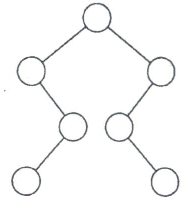
\includegraphics[width=0.3\textwidth]{../../figure/exercisePicPDF/chapter6/6-6.pdf}
            \caption{二叉树示意图}
    \end{figure}

    A. $c$  

    B. $d$  

    C. $f$  

    D. $g$  

    \item 已知字符集 $\{a, b, c, d, e, f, g, h\}$,若各字符的哈夫曼编码依次是 $0100, 10, 0000, 0101, 001, 011, 11, 0001$,则编码序列 $0100011001001011110101$ 的译码结果是( )。  
    【2017 年全国试题 6(2 分)】  

    A. $acgabfh$  

    B. $adbagbb$  

    C. $afbeagd$  

    D. $afeefgd$  

    \item 若森林已知有 15 条边、25 个结点,则森林包含树的个数是( )。  
    【2016 年全国试题 5(2 分)】 

    A. 8 \quad B. 9 \quad C. 10 \quad D. 11  

    \item 给定二叉树如下图所示。设 $W$ 代表二叉树的根,$L$ 代表根结点的左子树,$R$ 代表根结点的右子树。若遍历后的结点序列为 $3, 1, 7, 5, 6, 2, 4$,则其遍历方式是( )。  
    【2009 年全国试题 3(2 分)】  

    \begin{figure}[h!]
            \centering
            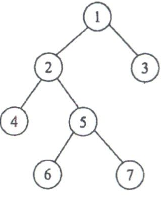
\includegraphics[width=0.3\textwidth]{../../figure/exercisePicPDF/chapter6/6-9.pdf}
            \caption{二叉树示意图}
    \end{figure}

    A. $LRN$ \quad B. $NRL$ \quad C. $RLN$ \quad D. $RNL$  

    \item 已知一棵完全二叉树的第 6 层(设根是第 1 层)有 8 个叶结点,则该完全二叉树的结点个数最多是( )。  
    【2009 年全国试题 5(2 分)】  

    A. 39 \quad B. 52 \quad C. 111 \quad D. 119  

    \item 将森林转换为对应的二叉树,若在二叉树中,结点 $z$ 是结点 $y$ 的父结点的父结点,则在原来的森林中,$z$ 和 $y$ 可能具有的关系是( )。  
    
    I. 父子关系  

    II. 兄弟关系  

    III. z 的父结点与 y 的父结点是兄弟关系  

    A. 只有 II  

    B. I 和 II  

    C. I 和 III  

    D. I 、II 和 III  

    \item 下列线索二叉树中(用虚线表示线索),符合后序线索树定义的是( )。  
    【2010 年全国试题 3(2 分)】  

    \begin{figure}[h!]
            \centering
            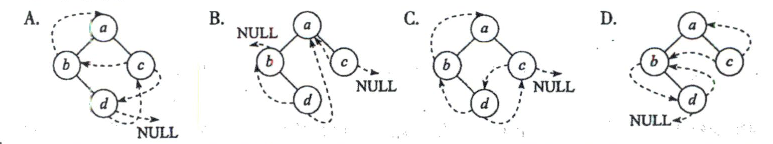
\includegraphics[width=1\textwidth]{../../figure/exercisePicPDF/chapter6/6-12.pdf}
            \caption{线索二叉树示意图}
    \end{figure}

    \item 在一棵度为 4 的树 $T$ 中,若有 20 个度为 4 的结点,10 个度为 3 的结点,1 个度为 2 的结点,10 个度为 1 的结点,则树 $T$ 的叶结点个数是( )。  
    【2010 年全国试题 5(2 分)】 

    A. 41 \quad B. 82 \quad C. 113 \quad D. 122  

    \item 对$n(n≥2)$个权值均不相同的字符构造哈夫曼树。下列关于哈夫曼树的叙述中,错误的是( )。  
    【2010 年全国试题 6(2 分)】  

    A. 是一棵完全二叉树  

    B. 树中一定没有度为 1 的结点  



    C. 树中两个权值最小的结点一定是兄弟结点

    D. 树中任一非叶结点的权值一定不小于下一层任一结点的权值  

    \item 若一棵完全二叉树有 768 个结点,则该二叉树中叶结点的个数是( )。  
    【2011 年全国试题 4(2 分)】  

    A. 257 \quad B. 258 \quad C. 384 \quad D. 385  

    \item 若一棵二叉树的前序遍历序列和后序遍历序列分别是 $1, 2, 3, 4$ 和 $4, 3, 2, 1$,则该二叉树的中序遍历序列不会是( )。  
    【2011 年全国试题 5(2 分)】  

    A. $1, 2, 3, 4$  

    B. $2, 3, 4, 1$  

    C. $3, 2, 4, 1$  

    D. $4, 3, 2, 1$  

    \item 已知一棵有 2011 个结点的树,其叶结点个数为 116,该树对应的二叉树中无右孩子的结点个数是( )。  
    【2011 年全国试题 6(2 分)】  

    A. 115 \quad B. 116 \quad C. 1895 \quad D. 1896  

    \item 若一棵二叉树的前序遍历序列为 $a,e,b,d,c$,后序遍历序列为 $b,c,d,e,a$,则根结点的孩子结点是( )。  
    【2012 年全国试题 3(2 分)】 

    A. 只有 $e$  

    B. 有 $e, b$  

    C. 有 $e, c$  

    D. 无法确定  

    \item 已知三叉树 $T$ 中 6 个叶结点的权分别是 $2, 3, 4, 5, 6, 7$,$T$ 的带权(外部)路径长度最小是( )。  
    【2013 年全国试题 4(2 分)】 

    A. 27 \quad B. 46 \quad C. 54 \quad D. 56  

    \item 若 $x$ 是后序线索二叉树中的叶结点,且 $x$ 存在左兄弟结点 $y$,则 $x$ 的右线索指向的是( )。  
    【2013 年全国试题 5(2 分)】 

    A. $x$ 的父结点  

    B. 以 $y$ 为根的子树的最左下结点  

    C. $x$ 的左兄弟结点 $y$  

    D. 以 $y$ 为根的子树的最右下结点  

    \item 若对如下图所示的二叉树进行中序线索化,则结点 $*$ 的左、右线索指向的结点分别是( )。  
    【2014 年全国试题 4(2 分)】
    \begin{figure}[h!]
            \centering
            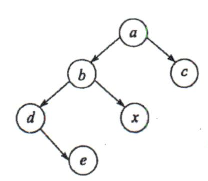
\includegraphics[width=0.15\textwidth]{../../figure/exercisePicPDF/chapter6/6-20.pdf}
            \caption{二叉树示意图}
    \end{figure}

    A. $c, c$ \quad B. $c, a$ \quad C. $d, c$ \quad D. $b, a$  

    \item 将森林 $F$ 转换为对应的二叉树 $T$,$F$ 中叶结点的个数等于( )。  
    【2014 年全国试题 5(2 分)】  

    A. $T$ 中叶结点的个数  

    B. $T$ 中度为 1 的结点个数  

    C. $T$ 中左孩子指针为空的结点个数  

    D. $T$ 中右孩子指针为空的结点个数  

    \item 5 个字符有如下 4 种编码方案,不是前缀编码的是( )。  
    【2014 年全国试题 6(2 分)】  

    A. $01, 0000, 0001, 001, 1$  

    B. $011, 000, 001, 010, 1$ 

    C. $000, 001, 010, 011, 100$  

    D. $0, 100, 110, 1110, 1100$  

    \item 先序序列为 $a, b, c, d$ 的不同二叉树的个数是( )。  
    【2015 年全国试题 2(2 分)】 

    A. 13 \quad B. 14 \quad C. 15 \quad D. 16  

    \item 下列选项给出的是从根分别到达两个叶结点路径上的权值序列,能属于同一棵哈夫曼树的是( )。  
    【2015 年全国试题 3(2 分)】  

    A. $24, 10, 5$ 和 $24, 10, 7$

    B. $24, 10, 5$ 和 $24, 12, 7$  

    C. $24, 10, 10$ 和 $24, 14, 11$  

    D. $24, 10, 5$ 和 $24, 14, 6$  

    \item 树是一种逻辑关系,表示数据元素之间存在的关系为( )。  
    【北京交通大学 2007(2 分)】  

    A. 集合关系  

    B. 一对一关系  

    C. 一对多关系  

    D. 多对多关系  

    \item 下列判断中,( )是正确的。  
    【华南理工大学 2005 一、1(2 分)】  

    A. 二叉树就是度为 2 的树  

    B. 二叉树中不存在度大于 2 的结点  

    C. 二叉树是有序树  

    D. 二叉树的每个结点的度都为 2  

    \item 有关二叉树的下列说法中,正确的是( )。  
    【南京理工大学 2000 一、11(1.5 分)】  

    A. 二叉树的度为 2  

    B. 一棵二叉树的度可以小于 2  

    C. 二叉树中至少有一个结点的度为 2  

    D. 二叉树中任何一个结点的度都为 2  

    \item 在下述结论中,正确的是( )。  
    【南京理工大学 1999 一、4(1 分)】 

    A. 只有一个结点的二叉树的度为 0  

    B. 二叉树的度为 2  

    C. 二叉树的左右子树可任意交换  

    D. 深度为 $d$ 的完全二叉树的结点个数小于或等于深度相同的满二叉树  

    \item 设有一表示算术表达式的二叉树(见下图),它所表示的算术表达式是( )。  
    【南京理工大学 1999 一、20(2 分);烟台大学 2007 一、11(2 分)】  

    \begin{figure}[h!]
        \centering
        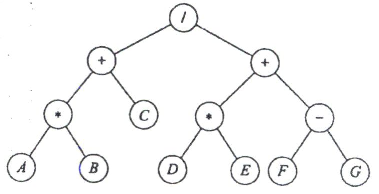
\includegraphics[width=0.3\textwidth]{../../figure/exercisePicPDF/chapter6/6-30.pdf}
        \caption{二叉树示意图}
    \end{figure}

    A. $A \ast B + C / (D \ast E) + (F - G)$  

    B. $(A \ast B + C) / (D \ast E) + (F - G)$  

    C. $(A \ast B + C) / (D \ast E) + (F - G)$  

    D. $A \ast B + C / D \ast E + F - G$  

    \item 已知一算术表达式的中缀表达式为 $a - (b + c/d) \ast e$,则其后序表达式为( )。
    
    A. $-a + b \ast c / d$  

    B. $-a + b \ast cd/e$  


    C. $-+*abc/de$  

    D. $abcd /+e*-$  

    \item 算术表达式 $a + b \ast (c + d / e)$ 转为后缀表达式后为( )。  
    【中山大学 1999 一、5(1 分)】  

    A. $a \, b + c \, d \, e / *$  

    B. $a \, b \, c \, d \, e /+ \ast +$ 

    C. $a \, b \, c \, d \, e / \ast + +$  

    D. $a \, b \, c \, d \, e \ast / + +$  
    \item 每个结点的度或者为 0 或者为 2 的二叉树称为正则二叉树。$n$ 个结点的正则二叉树中有( )个叶子。  
    【武汉理工大学 2004 一、11(3 分)】

     A. $\lceil \log_2 n \rceil$  

    B. $\frac{n - 1}{2}$  

    C. $\lceil \log_2 (n + 1) \rceil$  

    D. $\frac{n + 1}{2}$  

    \item 设树 $T$ 的度为 4,其中度为 1、2、3 和 4 的结点个数分别为 $4, 2, 1, 1$,则 $T$ 中的叶子数为( )。  
    【南京理工大学 2000 一、8(1.5 分)】  

    A. 5 \quad B. 6 \quad C. 7 \quad D. 8  

    \item 设有一个度为 3 的树,其叶结点数为 $n_0$,度为 1 的结点数为 $n_1$,度为 2 的结点数为 $n_2$,度为 3 的结点数为 $n_3$,则 $n_0, n_1, n_2, n_3$ 满足关系( )。  
    【电子科技大学 2005 一、4(1 分)】  

    A. $n_0 = n_2  + 1$ 

    B. $n_0 = n_2 + 2n_3 + 1$  

    C. $n_0 = n_2 + n_3 + 1$  

    D. $n_0 = n_1 + n_2 + n_3$  

    \item 在一棵三叉树中,度为 3 的结点数为 2 个,度为 2 的结点数为 1 个,度为 1 的结点数为 2 个,度为 0 的结点数为( )个。  
    【哈尔滨工业大学 2001 三、2(2 分)】  

    A. 4 \quad B. 5 \quad C. 6 \quad D. 7  

    \item 以下说法中,( )是正确的。  
    【华南理工大学 2006 一、12(2 分)】  

    A. 完全二叉树中,叶结点的双亲的左兄弟(如果存在)一定不是叶结点  

    B. 任何一棵二叉树,终端结点数为度为 2 的结点数加 1 

    C. 二叉树不适合用顺序结构存储  

    D. 结点表示序号第 $i$ 的二叉树,第 $i$ 个结点的左孩子(如果存在)的编号为 $2i$  

    \item 一棵有 124 个叶结点的完全二叉树,最多有( )个结点。  
    【中国科学技术大学 1995 十四、3(2 分)】  

    A. 247 \quad B. 248 \quad C. 249 \quad D. 251  

    \item 已知一棵完全二叉树中共有 626 个结点,叶子结点的个数应为( )。  
    【上海交通大学 2005 四、6(2 分)】  

    A. 311 \quad B. 312 \quad C. 313 \quad D. 314  

    \item 具有 300 个结点的二叉树,其高度至少应为( )。  
    【北京理工大学 2006 五、8(1 分)】  

    A. 6 \quad B. 7 \quad C. 8 \quad D. 9  

    \item 当结点数目一定时,具有最小深度的二叉树是( )。  
    【北京航空航天大学 2005】  

    A. 满二叉树  

    B. 完全二叉树  

    C. 链条二叉树  

    D. 二叉排序树  

    \item 二叉树的第 $i$ 层上最多含有结点数为( )。  
    【中山大学 1998 二、7(2 分);北京理工大学 2001 六、5(2 分)】  

    A. $2^i$  


    B. $2^{i-1} - 1$  

    C. $2^{i-1}$  

    D. $2^{i} - 1$  

    \item 从树根(第 0 层)起,自上到下,逐层从左到右给二叉树的所有结点从 1 开始编号,则完全二叉树的第 $k$ 层从左到右第 $i$ 个结点的编号为( )。  
    【电子科技大学 2005 一、6(1 分)】  

    A. $2^k + i - 1$  

    B. $2^{k} - i + 1$  

    C. $2^k + i + 1$  

    D. $2^{k} - i - 1$  

    \item 下列判断中,( )是正确的。  
    【华南理工大学 2006 一、2(2 分)】  

    A. 深度为 $h$ 的二叉树最多有 $2^h - 1$ 个结点($h > 1$),最少有 $h$ 个结点  

    B. 二叉树中不存在度大于 2 的结点  

    C. 对二叉树遍历是指先序、中序或后序遍历中的一种  

    D. 构造线索二叉树是为了方便找到每个结点的双亲  

    \item 一个具有 1025 个结点的二叉树的高度为( )。  
    【南京理工大学 1999 一、19(2 分)】  

    A. 10 \quad B. 10 \quad C. 11 至 1025 之间 \quad D. 10 至 1024 之间  

    \item 一棵二叉树高度为 $h$,所有结点的度或为 0,或为 2,则这棵二叉树最少有( )个结点。  
    【南京理工大学 2001 一、11(1.5 分);华中科技大学 2007 一、4(2 分);江苏大学 2004 一、6(2 分)】  

    A. $2h$ \quad B. $2h - 1$ \quad C. ${2h+1}$ \quad D. $h + 1$  

    \item 设二叉树中有 $n_2$ 个度为 2 的结点,有 $n_1$ 个度为 1 的结点,有 $n_0$ 个度为 0 的结点,则该二叉树中空指针个数为( )。  
    【重庆大学 2005】  

    A. $n_0 + n_1 + n_2$  

    B. $2n_0 + n_1 + n_2$  

    C. $2n_2 + n_1$  

    D. $2n_0 + n_1 $  

    \item 一棵具有 $n$ 个结点的完全二叉树的树高(深度)是( )。  
    【南京理工大学 1996 一、8(2 分)】  

    A. $\lfloor \log_2 n \rfloor + 1$  

    B. $ \log_2 n  + 1$ 

    C. $ \lfloor \log_2 n \rfloor$  

    D. $\log_2 n - 1$  

    \item 有 $n$($n > 0$)个结点的二叉树的深度的最小值是( )选项重复。  
    【华中科技大学 2006 一、6(2 分)】  

    A. $\lceil \log_2 n \rceil$  
    
    B. $\lceil \log_2 (n + 1) \rceil$  

    C. $\lfloor \log_2 (n + 1) \rfloor$  

    D. $\lceil \log_2 n \rceil$  

    \item 有 $n$ 个结点,并且高度为 $h$ 的二叉树的数目为( )。  
    【华中科技大学 2007 一、10(2 分)】 

    A. $\log_2 n$ \quad B. $n / 2$ \quad C. $n$ \quad D. $2^{n-1}$  

    \item 深度为 $h$ 的满m叉树的第 $k$ 层有( )个结点($1 \leq k \leq h$)。  
    【北京航空航天大学 2000 一、4(2 分)】  
    
    A. $m^{k-1}$ \quad B. $m^{k} - 1$ \quad C. $m^{h-1}$ \quad D. $m^{h} - 1$  

    \item 有 $n$($n > 0$)个分支结点的满二叉树的深度是( )。  
    【华中科技大学 2004 一、6(1 分)】  

    A. $n^2 - 1$ \quad B. $\log_2 (n + 1) + 1$ \quad C. $\log_2 (n + 1)$ \quad D. $\log_2 (n - 1)$  

    \item 深度为 $i$(设根的层数为 1)的完全二叉树至少包含的结点数目是( )。  
    【北京工业大学 2017 一、5(2 分)】  

    A. $2^{i-1}$ \quad B. $2^i$ \quad C. $2^{i - 1}$ \quad D. $2^{i-1} - 1$  

    \item 一棵深度为 4 的完全二叉树,最少有( )个结点。  
    【华南理工大学 2005 一、1(2 分)】  

    A. 4 \quad B. 8 \quad C. 15 \quad D. 6  

    \item 某完全二叉树的结点个数为 100,则第 60 个结点的度为( )。  
    【西南交通大学 2005】  

    A. 0 \quad B. 1 \quad C. 2 \quad D. 不确定  

    \item 若用一维数组表示一个深度为 5、结点个数为 10 的二叉树,数组的长度至少为( )。  
    【北京理工大学 2006 九、9(1 分)】 

    A. 10 \quad B. 16 \quad C. 31 \quad D. 64  

    \item 将有关二叉树的概念推广到三叉树,则一棵有 244 个结点的完全三叉树的高度为( )。  
    【南京理工大学 2000 一、5(1.5 分);烟台大学 2007 一、13(2 分)】 

    A. 4 \quad B. 5 \quad C. 6 \quad D. 7  

    \item 任何一棵二叉树的叶子结点在其先序、中序、后序遍历序列中的相对位置( )。  
    【北京交通大学 2006 一、3(2 分)】  

    A. 肯定发生变化  

    B. 有时发生变化  

    C. 肯定不发生变化  

    D. 无法确定  

    \item 在二叉树结点的先序序列、中序序列和后序序列中,所有叶子结点的先后顺序( )。  
    【北方交通大学 2001 一、25(2 分)】 

    A. 都不相同  

    B. 完全相同  

    C. 先序和中序相同,而与后序不同  

    D. 中序和后序相同,而与先序不同  

    \item 对二叉树的结点从 1 开始进行连续编号,要求每个结点的编号大于其左、右孩子的编号,同一结点的左右孩子中,其左孩子的编号小于其右孩子的编号,可采用( )次序的遍历实现编号。  
    【北京理工大学 2000 一、4(2 分);南开大学 2005】  

    A. 先序  

    B. 中序  

    C. 后序  

    D. 从根开始按层次遍历  

    \item 若二叉树采用二叉链表存储结构,要交换其所有分支结点左、右子树的位置,利用( )遍历方法最合适。  
    【北京航空航天大学 1999 一、4(2 分)】

    A. 前序  

    B. 中序  

    C. 后序  



    D. 按层次  

    \item 下面不能唯一确定一棵二叉树的两个遍历序列是( )。  
    【北京理工大学 2006 九、10(1 分)】  

    A. 先序序列和中序序列  

    B. 先序序列和后序序列  

    C. 后序序列和中序序列 

    D. 都不能  

    \item 根据( )可以唯一地确定一棵二叉树。  
    【北京理工大学 2005 一、8(1 分)】  

    A. 先序遍历和后序遍历  

    B. 先序遍历和层次遍历  

    C. 中序遍历和层次遍历  

    D. 中序遍历和后序遍历  

    \item 一棵有 $n$ 个结点的二叉树,按层次从上到下、同一层从左到右顺序存储在一维数组 $A[1..m]$ 中,则二叉树中第 $i$ 个结点($i$ 从 1 开始用上述方法编号)的右孩子在数组 $A$ 中的位置是( )。  
    【南京理工大学 2000 一、4(1.5 分)】  

    A. $A[2i]$($2i ≤ n$)  

    B. $A[2i+1]$($2i+1 ≤ n$) 

    C. $A[i-2]$  

    D. 条件不充分,无法确定  

    \item 设 $m, n$ 为一棵二叉树上的两个结点,在中序遍历时,$m$ 在 $n$ 前的条件是( )。  
    【北京理工大学 2006 五、9(1 分)】  

    A. $m$ 在 $n$ 的右方 

    B. $m$ 是 $n$ 的祖先  

    C. $m$ 在 $n$ 的左方  

    D. $m$ 是 $n$ 的子孙  

    \item 一棵二叉树的前序遍历序列为 $A, B, C, D, E, F, G$,它的中序遍历序列可能是( )。  
    【北京工业大学 2001 一、2(2 分)】 

    A. $C, A, B, D, E, F, G$  

    B. $A, B, C, D, E, F, G$  

    C. $D, A, C, E, F, B, G$  

    D. $A, D, C, F, E, G$  

    \item 已知一棵二叉树的前序遍历结果为 $ABCDEF$,中序遍历结果为 $CBAEDF$,则后序遍历的结果为( )。  
    【浙江大学 1999 四、2(4 分)】  

    A. $ CBEFDA$ \quad B. $FEDCBA $ \quad C. $CBEDFA $ \quad D. 不定  

    \item 某二叉树的先序遍历序列为 $IJKLMNO$,中序遍历序列为 $JLKINMO$,则后序遍历序列是( )。  
    【北京大学 2016 一、5(2 分)】  

    A. $JLKMNOI$ \quad B. $LKNJOMI$ \quad C. $LKJNOMI$ \quad D. $LKNOJMI$  

    \item 某二叉树中序序列为 $A, B, C, D, E, F,G$,后序序列为 $B, D, C, A,F, G, E$,则前序序列是( )。  
    【南京理工大学 2000 一、14(1.5 分)】  

    A. $E, G, F, A, C, D,B$  

    B. $E,A,C,B,D,G,F$  

    C. $E,A,G,C,F,B,D$  

    D. 上面的都不对  

    \item 一棵二叉树中序序列为 $FEABDC$,后序序列为 $FBADCE$,则层序序列为( )。  
    【华南理工大学 2006 一、11(2 分)】  

    A. $ABCDEF$ \quad B. $EFCDBA$ \quad C. $FECDAB$ \quad D. $EFCDAB$  

    \item 某二叉树结点的中序序列为 $BDAECF$,后序序列为 $DBEFCA$,则该二叉树对应的森林包括( )棵树。  
    【中南大学 2003 二、8(1 分)】  

    A. 1 \quad B. 2 \quad C. 3 \quad D. 4  

    \item 二叉树的先序遍历和中序遍历如下:先序遍历 $EFHIGJK$;中序遍历 $HFIEJKG$。该二叉树根的右子树的根是( )。  
    【北方交通大学 2001 一、21(2 分)】  

    A. $E$ \quad B. $F$ \quad C. $G$ \quad D. $H$  

    \item 对于前序遍历与中序遍历结果相同的三叉树为(1),对于前序遍历和后序遍历结果相同的二叉树为(2)。  
    【中科院计算所 1999 一、4(4 分)】  

    A. 一般二叉树  

    B. 只有根结点的二叉树  

    C. 根结点无左孩子的二叉树  

    D. 根结点无右孩子的二叉树  

    E. 所有结点只有左子树的二叉树 

    F. 所有结点只有右子树的二叉树  

    \item 前序遍历和后序遍历结果相同的二叉树为(1)。  
    
    前序遍历和中序遍历结果相同的二叉树为(2)。

    中序遍历和后序遍历结果相同的二叉树为(3)。 

    【南京理工大学 2005 一、6(1 分)】  

    A. 一般二叉树  

    B. 空树或根结点无左孩子的二叉树  

    C. 空树或只有根结点的二叉树  

    D. 空树或根结点无右孩子的二叉树  

    E. 空树或缺左子树的单支二叉树  

    F. 空树或缺右子树的单支二叉树  

    \item 一棵非空的二叉树的先序序列和后序序列正好相反,则该二叉树一定满足( )。  
    【中南大学 2005 一、7(2 分)】  

    A. 其中任意一个结点均无左孩子 

    B. 其中任意一个结点均无右孩子  

    C. 其中只有一个叶子结点  

    D. 其中度为 2 的结点最多为一个  

    \item 某二叉树的前序序列和中序序列正好相反,则该二叉树一定具有( )的特征(多项选择)。  
    【华东师范大学 2004】  

    A. 二叉树为空或只有一个结点  

    B. 若二叉树不为空,则任一结点不能同时拥有左孩子和右孩子 

    C. 若二叉树不为空,则任一结点没有左孩子 

    D. 若二叉树不为空,则任一结点没有右孩子  

    \item 某二叉树的先序和后序遍历次序正好相反,则该二叉树一定是( )二叉树。  
    【吉林大学 2016 一、2(2 分)】  

    A. 空或只有一个结点  

    B. 高度等于其结点数  

    C. 任意结点无左孩子  

    D. 任意结点无右孩子  

    \item 一棵非空二叉树的先序序列和后序序列正好相反,当且仅当( )。  
    【华中科技大学 2007 一、2(2 分)】  

    A. 二叉树任意一结点都无左孩子  

    B. 二叉树任意一结点都无右孩子  

    C. 二叉树只有一个叶子结点  

    D. 二叉树只有一个根结点  

    \item 在完全二叉树中,若一个结点是叶结点,则它没有( )。  
    【北方交通大学 2001 一、22(2 分)】  

    A. 左子结点  

    B. 右子结点  

    C. 左子结点和右子结点  

    D. 左子结点、右子结点和兄弟结点  

    \item 在下列存储形式中,哪一个不是树的存储形式( )。  
    【北方交通大学 2001 一、23(2 分)】  

    A. 双亲表示法  

    B. 孩子链表表示法  

    C. 孩子兄弟表示法  

    D. 顺序存储表示法  

    \item 树的后根遍历序列等同于该树对应的二叉树的( )。  
    【北京理工大学 2001 六、6(2 分)】  

    A. 先序序列  

    B. 中序序列  

    C. 后序序列  

    \item 将一棵树转换为孩子-兄弟链表表示的二叉树,则该树的后根序遍历是该二叉树的( )。  
    【北京邮电大学 2001 一、2(2 分)】  

    A. 前序遍历  

    B. 中序遍历  

    C. 后序遍历  

    \item 对任意一棵树,设它有 $n$ 个结点,这 $n$ 个结点的度数之和为( )。  
    【南京邮电学院 2004 一、3(3 分)】  

    A. $n$  

    B. $n - 2$  

    C. $n - 1$  

    D. $n + 1$  

    \item 高度为 $h (> 0)$ 的满二叉树对应的森林由( )棵树构成。  
    【北京交通大学 2004 一、9(2 分)】  

    A. $1$  

    B. $\log2^h$  

    C. $h/2$  

    D. $h$  

    \item 在下列情况中,可称为二叉树的是( )。  
    【西安交通大学 1996 三、4(3 分)】  

    A. 每个结点至多有两棵子树的树  

    B. 哈夫曼树  

    C. 每个结点至多有两棵子树的有序树  

    D. 每个结点只有一棵右子树  

    \item 一棵完全二叉树又是一棵( )。  
    【华中科技大学 2006 一、7(2 分)】  

    A. 平衡二叉树  

    B. 堆  

    C. 二叉排序树  

    D. 哈夫曼树  

    \item 一棵左子树为空的二叉树在先序线索化后,其中空的链域的个数是( )。  
    【合肥工业大学 1999 一、5(2 分)】 

    A. 不确定  

    B. 0  

    C. 1  

    D. 2  

    \item 一棵左右子树均不空的二叉树在先序线索化后,其中空的链域的个数是( )。  
    【合肥工业大学 2000 一、5(2 分)】  

    A. 0  

    B. 1 

    C. 2  

    D. 不确定  

    \item 若某中序线索树中一个有左孩子的结点,且该结点不为根,则该结点的前驱为( )。  
    【南京理工大学 1996 一、6(2 分)】  

    A. 该结点的双亲  

    B. 该结点的右子树中最左的结点  

    C. 该结点的左子树中最右的结点  

    D. 该结点的左子树中最右叶结点  

    \item 引入二叉线索树的目的是( )。  
    【南京理工大学 1998 一、5(2 分)】

    A. 加快查找结点的前驱或后继的速度  

    B. 为了能在二叉树中方便地进行插入与删除  

    C. 为了能方便地找到双亲  

    D. 以上都不是  

    \item $n$ 个结点的线索二叉树上含有的线索数为( )。  
    【中山大学 1998 二、8(2 分)】  

    A. $2n$  

    B. $n - 1$  

    C. $n+1$  

    D. $n$  

    \item ( )的遍历仍需要栈的支持。  
    【中科院计算所 1999 一、1(2 分)】  

    A. 前序线索树  

    B. 中序线索树  

    C. 后序线索树  

    \item 二叉树在线索化后,仍不能有效求解的问题是( )。  
    【北方交通大学 2003 一、4(2 分)】 

    A. 先序线索二叉树中求先序后继  

    B. 中序线索二叉树中求中序后继  

    C. 中序线索二叉树中求中序前驱 

    D. 后序线索二叉树中求后序后继  

    \item 在线索二叉树中,下面说法不正确的是( )。  
    【南京理工大学 2004 一、8(1 分)】  

    A. 在中序线索树中,若某结点有右孩子,则其后继结点是它的右子树的左支末端结点  

    B. 线索二叉树是利用二叉树的 $n + 1$ 个空指针来存放结点前驱和后继信息的  

    C. 每个结点通过线索都可以直接找到它的前驱和后继 

    D. 在中序线索树中,若某结点有左孩子,则其前驱结点是它的左子树的右支末端结点  

    \item 采用双亲表示法表示树,则具有 $n$ 个结点的树至少需要( )个指向双亲的指针。  
    【中山大学 2004】  

    A. $n$ \quad B. $n + 1$ \quad C. $n - 1$ \quad D. $2n$  

    \item 树用孩子兄弟表示法,每个结点有两个指针域,分别指向“第一个孩子”和“下一个兄弟”。若指向“下一个兄弟”的指针有 $m$ 个为空,则该树有( )个非终端结点。  
    【哈尔滨工程大学 2004】  

    A. $\lfloor m / 2 \rfloor$ \quad B. $m - 1$ \quad C. $m$ \quad D. $m + 1$  

    \item 由包含 $n$ 个结点的森林转换得到二叉树 $B$,$P$ 是指向二叉树 $B$ 的树根的指针,$P$ 的右子树结点个数是 $m$,则森林中第一棵树包含的结点数目是( )。  
    【北京工业大学 2017 一、6(2 分)】  

    A. $m - 1$ \quad B. $m + 1$ \quad C. $n - m$ \quad D. $n - m + 1$  

    \item 设森林 $F$ 中有三棵树,第一、第二、第三棵树的结点个数分别为 $M_1, M_2, M_3$,与森林 $F$ 对应的二叉树根结点的右子树上的结点个数是( )。  
    【北方交通大学 2001 一、16(2 分)】  

    A. $M_1$ \quad B. $M_1 + M_2$ \quad C. $M_3$ \quad D. $M_2 + M_3$  

    \item 设森林 $F$ 是由二叉树 $T$ 转换得到的,若 $T$ 中有 $n$ 个非终端结点,则 $F$ 中右指针域为空的结点有( )个。  
    【西安电子科技大学 1998 一、10(2 分)】  

    A. $n - 1$ \quad B. $n$ \quad C. $n + 1$ \quad D. $n + 2$  

    \item 如果二叉树 $T$ 是由有序树 $F$ 转换而来的二叉树,那么 $F$ 中结点的后序就是 $T$ 中结点的( )。  
    【西安电子科技大学 1996 一、2(2 分);电子科技大学 2005 一、7(1 分)】  

    A. 先序 \quad B. 中序 \quad C. 后序 \quad D. 层次序  

    \item 由 3 个结点可以构造出( )种不同的有向树。  
    【北方交通大学 2001 一、6(2 分)】  

    A. 2 \quad B. 3 \quad C. 4 \quad D. 5  

    \item 含有 4 个结点的二叉树有( )种树形。  
    【北京邮电大学 2005 一、5(2 分)】  

    A. 4 \quad B. 5 \quad C. 10 \quad D. 14  

    \item 由 3 个结点可以构造出( )种不同的二叉树。  
    【北方交通大学 2001 一、7(2 分)】  

    A. 2 \quad B. 3 \quad C. 4 \quad D. 5  

    \item 一棵共有 $n$ 个结点的树,其中所有分支结点的度均为 $k$,则该树中叶子结点的个数为( )。  
    【华南理工大学 2005 一、1(2 分)】  

    A. $\frac{n(k-1)}{k}$ \quad B. $n/k$ \quad C. $\frac{n + 1}{k}$ \quad D. $\frac{nk - n + 1}{k}$  

    \item 下述二叉树中,哪一种满足性质:从任一结点出发到根的路径上所经过的结点序列按其关键字有序。( )  
    【中国科技大学 1998 二、8(2 分);中科院计算所 1998 二、8(2 分);北京工业大学 2005 一、5(2 分);电子科技大学 2005 一、1(1 分);南京理工大学 2004 一、10(1 分)】  
    
    A. 二叉排序树 \quad B. 哈夫曼树 \quad C. AVL 树 \quad D. 堆  

    \item 具有 $n$ 个结点,其路径长度最短的二叉树是( )。  
    【电子科技大学 2005 一、3(1 分)】 

    A. 哈夫曼树 \quad B. 完全二叉树 \quad C. AVL 树 \quad D. 二叉排序树  

    \item 在叶子数目和权值相同的所有二叉树中,最优二叉树一定是完全二叉树,该说法( )。  
    【中国科技大学 1998 二、10(2 分);中科院计算所 1998 二、10(2 分)】 

    A. 正确 \quad B. 错误  

    \item 设二叉树只有度为 0 和 2 的结点,其结点个数是 15,则该二叉树最大深度为( )。  
    【北京理工大学 2007 一、8(1 分)】  

    A. 4 \quad B. 5 \quad C. 8 \quad D. 9  

    \item 一棵哈夫曼树共有 215 个结点,对其进行哈夫曼编码,共能得到( )个不同的码字。  
    【北京邮电大学 2005 一、6(2 分)】  

    A. 107 \quad B. 108 \quad C. 214 \quad D. 215  

    \item 设哈夫曼编码的长度不超过 4,若已对两个字符编码为 1 和 01,则还可以对( )字符编码。  
    【哈尔滨工程大学 2005】  

    A. 2 \quad B. 3 \quad C. 4 \quad D. 5  

    \item 若度为 $m$ 的哈夫曼树中,其叶结点个数为 $n$,则非叶结点的个数为( )。  
    【中科院计算所 1999 一、2(2 分)】  

    A. $n - 1$ \quad 
    
    B. $\lfloor n / (m) \rfloor - 1$  

    C. $\lceil (n - 1) / (m - 1) \rceil$ \quad 
    
    D. $\lceil n  / (m - 1) \rceil - 1$  

    E. $\lceil(n + 1)/(m + 1)-1$
    \item 下述编码中( )不是前缀码。  
    【中科院计算所 2000 一、2(2 分)】  

    A. $\{00, 01, 10, 11\}$  

    B. $\{0, 1, 00, 11\}$  

    C. $\{0, 10, 110, 111\}$  

    D. $\{1, 01, 000, 001\}$  

    \item 下述编码中( )不是前缀码。  
    【哈尔滨工业大学 2004 二、1(1 分);2005 二、1(1 分)】  

    A. $\{00, 01, 10, 11\}$  

    B. $\{10, 1, 00, 11\}$  

    C. $\{10, 10, 110, 111\}$  

    D. $\{000, 001, 010, 101\}$  

    \item 下列编码中,( )不是前缀码。  
    【湖南大学 2003】  

    A. $\{100, 01, 10, 111\}$  

    B. $\{10, 1, 00, 11\}$  

    C. $\{10, 10, 110, 111\}$  

    D. $\{110, 110, 1110, 1111\}$  

    \item 有 5 个字符,根据其使用频率设计对应的哈夫曼编码,以下( )是可能的哈夫曼编码。  
    【武汉大学 2006】  

    A. $\{000, 001, 010, 011, 11\}$  

    B. $\{0000, 0001, 001, 01, 1\}$  

    C. $\{000, 001, 01, 10, 11\}$  

    D. $\{00, 100, 101, 110, 111\}$  

    \item 现有一“遗传”关系,设 $x$ 是 $y$ 的父亲,则 $x$ 可以把它的属性遗传给 $y$,表示该遗传关系最适合的数据结构为( )。  
    【中国科学院 2006】  

    A. 向量 \quad B. 树 \quad C. 图 \quad D. 二叉树  

    \item 一棵深度为 7 的满二叉树共有( )个非终端结点。  
    【北京邮电大学 2007】  

    A. 31 \quad B. 63 \quad C. 127 \quad D. 35  

    \item 构建一个哈夫曼树,如果给定权值的个数为 $n$,那么哈夫曼树的结点总数为( )。  
    【北京大学 2016 一、6(2 分)】

    A. $n$ \quad B. $2n$ \quad C. $2n + 1$ \quad D. $2n - 1$  

    \item 有一棵包含 101 个结点的二叉树,度为 1 的结点数量为 30,则叶子结点的数量是( )。  
    【北京工业大学 2018 一、3(2 分)】 

    A. 16 \quad B. 26 \quad C. 36 \quad D. 46  

    \item 在一棵度为 5 的树 $T$ 中,包含 20 个度为 5 的结点,15 个度为 4 的结点,10 个度为 3 的结点,5 个度为 2 的结点,20 个度为 1 的结点,则 $T$ 中叶子结点的数量是( )。  
    【北京工业大学 2018 一、5(2 分)】 

    A. 140 \quad B. 141 \quad C. 150 \quad D. 151  

    \item 若一棵满二叉树有 2047 个结点,则该二叉树中非叶子结点的个数为( )。  
    【吉林大学 2017 一、3(2 分)】

    A. 512 \quad B. 1023 \quad C. 1024 \quad D. 1025 



\end{enumerate}


\chapter{图与网络}


\begin{enumerate}
    \item 右图所示的 AOE 网表示一项包含 8 个活动的工程。活动 4 的最早开始时间和最迟开始时间分别是( )。  
    【2019 年全国试题 5(2 分)】  
    \begin{figure}[h!]
            \centering
            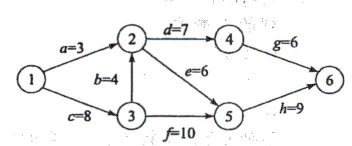
\includegraphics[width=0.5\textwidth]{../../figure/exercisePicPDF/chapter7/7-1.pdf}
            \caption{AOE 网}
    \end{figure}

    A. 3 和 7 \quad B. 12 和 12 \quad C. 12 和 14 \quad D. 15 和 15  

    \item 用有向无环图描述表达式 $(x + y) \ast ((x + y) / x)$,需要的顶点个数至少是( )。  
    【2019 年全国试题 6(2 分)】  

    A. 5 \quad B. 6  C. 8 \quad D. 9    

    \item 下列选项中,不是下图的拓扑排序的是( )。  
    【2018 年全国试题 7(2 分)】  

    \begin{figure}[h!]
            \centering
            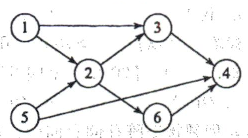
\includegraphics[width=0.5\textwidth]{../../figure/exercisePicPDF/chapter7/7-3.pdf}
            \caption{拓扑排序}
    \end{figure}

    A. $1, 5, 2, 3, 6, 4$  

    B. $5, 1, 2, 6, 3, 4$  

    C. $5, 1, 2, 3, 6, 4$  

    D. $5, 2, 1, 6, 3, 4$  

    \item 已知无向图 $G$ 含有 16 条边,其中度为 4 的顶点个数为 3,度为 3 的顶点个数为 4,其他顶点的度均小于 3。图 $G$ 所含的顶点个数至少是( )。  
    【2017 年全国试题 7(2 分);湖南大学 2006】 

    A. 10 \quad B. 11 \quad C. 13 \quad D. 15  

    \item 下列选项中,不是下图深度优先搜索序列的是( )。  
    【2016 年全国试题 6(2 分)】  

    \begin{figure}[h!]
            \centering
            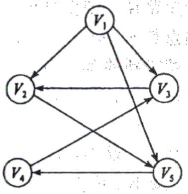
\includegraphics[width=0.3\textwidth]{../../figure/exercisePicPDF/chapter7/7-5.pdf}
            \caption{深度优先搜索}
    \end{figure}

        A. $V_1, V_5, V_4, V_3, V_2$  

        B. $V_1, V_3, V_2, V_5, V_4$  

        C. $V_1, V_2, V_5, V_4, V_3$  

        D. $V_1, V_2, V_3, V_4, V_5$  


    \item 若将 $n$ 个顶点、$e$ 条弧的有向图进行拓扑排序,则拓扑排序算法的时间复杂度是( )。  
    【2016 年全国试题 7(2 分)】  

    A. $O(n)$ \quad B. $O(n + e)$ \quad C. $O(n^2)$ \quad D. $O(n \times e)$  

    \item 使用迪杰斯特拉(Dijkstra)算法求图\ref{fig:7-7}中从顶点 1 到目标顶点的最短路径,目标顶点是( )。  
    【2016 年全国试题 8(2 分)】 
    
    \begin{figure}[h!]
            \centering
            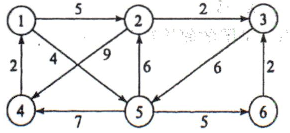
\includegraphics[width=0.5\textwidth]{../../figure/exercisePicPDF/chapter7/7-7.pdf}
            \caption{最短路径}
            \label{fig:7-7}
    \end{figure}

        A. $5, 2, 3, 4, 6$  

        B. $5, 2, 3, 6, 4$  

        C. $5, 2, 4, 3, 6$  

        D. $5, 2, 6, 3, 4$  


        \item 下列关于无向连通图特性的叙述中,正确的是( )。  
        【2009 年全国试题 7(2 分)】 

        I. 所有顶点的度之和为偶数  

        II. 边数大于顶点个数减 1  

        III. 至少有一个顶点的度为 1  

        A. 只有 I \quad B. 只有 II \quad C. I 和 II \quad D. I、II 和 III  
    
        \item 若无向图 $G = (V, E)$ 中含有 7 个顶点,要保证图 $G$ 在任何情况下都是连通的,需要的边数最少是( )。  
        【2010 年全国试题 7(2 分)】  

        A. 6 \quad B. 15 \quad C. 16 \quad D. 21  
    
        \item 对右图进行拓扑排序,可以得到不同拓扑序列的个数是( )。  
        【2010 年全国试题 8(2 分)】  

        \begin{figure}[h!]
            \centering
            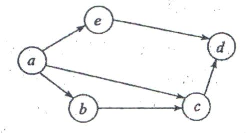
\includegraphics[width=0.5\textwidth]{../../figure/exercisePicPDF/chapter7/7-10.pdf}
            \caption{拓扑排序}
        \end{figure}

        A. 4 \quad B. 3 \quad C. 2 \quad D. 1  
    
        \item 下列关于图的叙述中,正确的是( )。  
        【2011 年全国试题 8(2 分)】  

        I. 回路是简单路径  

        II. 存储稀疏图,用邻接矩阵比邻接表更省空间  

        III. 若有向图中存在拓扑序列,则该图不存在回路  

        A. 仅 I \quad B. 仅 II、III \quad C. 仅 III \quad D. 仅 I、III  
    
        \item 对有 $n$ 个结点、$e$ 条边且使用邻接表存储的有向图进行广度优先遍历,其算法时间复杂度是( )。  
        【2012 年全国试题 5(2 分)】  

        A. $O(n)$ \quad B. $O(e)$ \quad C. $O(n + e)$ \quad D. $O(n \times e)$  
    
        \item 若用邻接矩阵存储有向图,且矩阵中主对角线以下的元素均为零,则关于该图拓扑序列的结论是( )。  
        【2012 年全国试题 6(2 分)】  

        A. 存在,且唯一  

        B. 存在,且不唯一  

        C. 存在,可能不唯一  

        D. 无法确定是否存在  
    
        \item 对如右图所示有向带权图,若采用迪杰斯特拉(Dijkstra)算法求从源点 $a$ 到其他各顶点的最短路径,则得到的第一条最短路径的目标顶点是 $b$,第二条最短路径的目标顶点是 $c$,后续得到的其余各最短路径的目标顶点依次是( )。  
        【2012 年全国试题 7(2 分)】  

        \begin{figure}[h!]
            \centering
            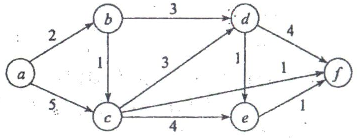
\includegraphics[width=0.5\textwidth]{../../figure/exercisePicPDF/chapter7/7-14.pdf}
            \caption{最短路径}
    \end{figure}
        A. $d,e,f$ \quad B. $e, d, f$ \quad C. $f,d, e$ \quad D. $f,e,d$  
    
        \item 下列关于最小生成树的叙述中,正确的是( )。  
        【2012 年全国试题 8(2 分)】  

        I. 最小生成树的代价唯一  

        II. 所有权值最小的边一定会出现在所有的最小生成树中 

        III. 使用普里姆(Prim)算法从不同顶点开始得到的最小生成树一定相同  

        IV. 使用普里姆算法和克鲁斯卡尔(Kruskal)算法得到的最小生成树总不相同  

        A. 仅 I \quad B. 仅 II \quad C. 仅 II、III \quad D. 仅 II、IV  
    
        \item 设图的邻接矩阵 $A$ 如下所示,各顶点的度依次是( )。  
        【2013 年全国试题 7(2 分)】  

        \[
        A = 
        \begin{bmatrix}
        0 & 1 & 1 & 0 \\
        1 & 0 & 1 & 1 \\
        1 & 1 & 0 & 0 \\
        0 & 1 & 0 & 0
        \end{bmatrix}
        \]  

        A. $3, 3, 2, 1$ \quad B. $3, 4, 2, 1$ \quad C. $3, 4, 2, 3$ \quad D. $4, 4, 2, 2$  


        \item 若对图\ref{fig:7-17}所示的无向图进行便利,下列选项中,不是广度优先遍历序列的是( )。  
        【2013 年全国试题 8(2 分)】  


        \begin{figure}[h!]
            \centering
            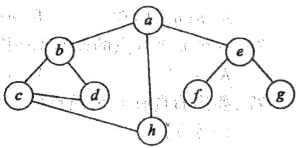
\includegraphics[width=0.5\textwidth]{../../figure/exercisePicPDF/chapter7/7-17.pdf}
            \caption{广度优先遍历}
            \label{fig:7-17}
    \end{figure}
    A. h, c, a, b, d, e, g, f  

    B. e, a, f, g, b, h, c, d 

    C. d, b, c, a, h, e, f, g  

    D. a, b, c, d, h, e, f, g  
    
        \item 图\ref{fig:7-18}所示 AOE 网表示一项包含 8 个活动的工程。通过同时加快若干活动的进度可以缩短整个工程的工期的是( )。  
        【2013 年全国试题 9(2 分)】  

        \begin{figure}[h!]
            \centering
            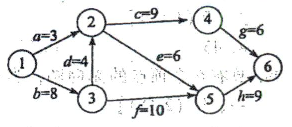
\includegraphics[width=0.5\textwidth]{../../figure/exercisePicPDF/chapter7/7-18.pdf}
            \caption{AOE 网}
            \label{fig:7-18}
    \end{figure}

        A. $c$ 和 $e$  

        B. $d$ 和 $e$  

        C. $f$ 和 $d$  

        D. $j$ 和 $d$  
    
        \item 对如图\ref{fig:7-19}所示的有向图进行拓扑排序,得到的拓扑序列可能是( )。  
        【2014 年全国试题 7(2 分)】  

        \begin{figure}[h!]
            \centering
            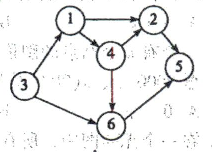
\includegraphics[width=0.5\textwidth]{../../figure/exercisePicPDF/chapter7/7-19.pdf}
            \caption{拓扑排序}
            \label{fig:7-19}
    \end{figure}

        A. $3, 1, 2, 4, 6, 5$  

        B. $3, 1, 2, 4, 6, 5$  

        C. $3, 1, 4, 2, 5, 6$  

        D. $3, 1, 4, 2, 6, 5$  
    
        \item 设有向图 $G = (V, E)$,顶点集 $V = \{v_0,v_1, v_2, v_3\}$,边集 $E = \{(v_0, v_1), (v_0, v_2), (v_0, v_3),(v_1,v_2)\}$,若从顶点 $v_0$ 开始遍历,则可能得到的不同遍历序列个数是( )。  
        【2015 年全国试题 5(2 分)】  

        A. 2 \quad B. 3 \quad C. 4 \quad D. 5  
    
        \item 求图\ref{fig:7-21}所示带权图的最小(代价)生成树时,可能是克鲁斯卡尔(Kruskal)算法第二次选中但不是普里姆(Prim)算法(从 $v_1$ 开始)第二次选中的边是( )。  
        【2015 年全国试题 6(2 分)】  

        \begin{figure}[h!]
            \centering
            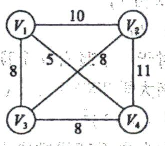
\includegraphics[width=0.3\textwidth]{../../figure/exercisePicPDF/chapter7/7-21.pdf}
            \caption{最小生成树}
            \label{fig:7-21}
        \end{figure}

        A. $(v_1, v_3)$ \quad B. $(v_1, v_4)$ \quad C. $(v_2, v_3)$ \quad D. $(v_3, v_4)$  
    
        \item 以下关于图的叙述中,正确的是( )。  
        【华南理工大学 2006 一、(2 分)】  

        A. 图与树的区别在于图的边数大于或等于顶点数  

        B. 假设有图 $G = (V, E)$,顶点集 $V \subseteq V'$,边集 $E \subseteq E'$,则 $V$ 和 $E$ 构成 $G$ 的子图  

        C. 无向图的连通分量指无向图中的极大连通子图  

        D. 图的遍历就是从图中某一顶点出发访问图中其余顶点  
    
        \item 有关图中路径的定义,表述正确的是( )。  
        【烟台大学 2019 一、10(2 分)】  

        A. 路径是顶点和相邻顶点偶对构成的边所形成的序列  

        B. 路径是图中相邻顶点的序列  

        C. 路径是不同边所形成的序列  

        D. 路径是不同顶点和不同边所形成的集合  
    
        \item 设无向图的顶点个数为 $n$,则该图最多有( )条边。  
        【清华大学 1998 一、5(2 分)】  

        A. $n - 1$ \quad B. $\frac{n(n-1)}{2}$ \quad C. $\frac{n(n+1)}{2}$ \quad D. $n^2$ 


        \item 具有 $n$ 个顶点的有向完全图有( )条边。  
        【湖南大学 2008】  

        A. $\frac{n(n-1)}{2}$ \quad B. $n(n-1)$ \quad C. $\frac{n(n+1)}{2}$ \quad D. $n(n+1)$  
    
        \item 一个 $n$ 个顶点的连通无向图,其边的个数至少为( )。  
        【浙江大学 1999 四、4(4 分)】  

        A. $n-1$ \quad B. $n$ \quad C. $n+1$ \quad D. $n \log n$  
    
        \item 要连通具有 $n$ 个顶点的有向图,至少需要( )条边。  
        【北京航空航天大学 2000 一、6(2 分)】  

        A. $n-1$ \quad B. $n$ \quad C. $n+1$ \quad D. $2n$  
    
        \item 设有向图 $G$ 是有 10 个顶点的强连通图,则 $G$ 至少有( )条边。  
        【哈尔滨工业大学 2005】  

        A. 45 \quad B. 90 \quad C. 10 \quad D. 9  
    
        \item 具有 6 个顶点的无向图,当有( )条边时能确保是一个连通图。  
        【华中科技大学 2007 一、11(2 分)】  

        A. 8 \quad B. 9 \quad C. 10 \quad D. 11  
    
        \item 一个 $n$ 个结点的完全有向图含有的边的数目是( )。  
        【中山大学 1998 二、9(2 分)】 

        A. $n*n$ \quad B. $n(n+1)$ \quad C. $\frac{n}{2}$ \quad D. $n(n-1)$  
    
        \item 一个有 $n$ 个结点的图最少有( )个连通分量,最多有( )个连通分量。  
        【北京邮电大学 2000 二、5(2 分)】  

        A. 0 \quad B. 1 \quad C. $n-1$ \quad D. $n$  
    
        \item 在一个无向图中,所有顶点的度数之和等于所有边数之和的( )倍;在一个有向图中,所有顶点的入度之和等于所有顶点出度之和的( )倍。  
        【哈尔滨工业大学 2001 二、3(2 分)】 

        A. $1/2$ \quad B. 2 \quad C. 1 \quad D. 4  
    
        \item 一个有向图共有 $m$ 条弧,则所有顶点的度的总和为( )。  
        【华南理工大学 2006 一、9(2 分)】  

        A. $2m$ \quad B. $m$ \quad C. $m-1$ \quad D. $m/2$  
    
        \item 对于一个具有 $n$ 个顶点的无向图,若采用邻接矩阵表示,则该矩阵的大小为( )。  
        【中南大学 2005 一、5(2 分)】  

        A. $(n-1)^2$ \quad B. $n^2$ \quad C. $n-1$ \quad D. $n$  
    
        \item 用有向无环图描述表达式 $(a+b) \ast ((a+b)/a)$,至少需要顶点的数目为( )。  
        【中山大学 1999 一、14】  

        A. 5 \quad B. 6 \quad C. 8 \quad D. 9  
    
        \item 无向网(加权图)的邻接矩阵是( )矩阵。  
        【华中科技大学 2006 一、8(2 分)】  

        A. 下三角 \quad B. 上三角 \quad C. 稀疏 \quad D. 对称  
    
        \item 设有两个无向图 $G = (V, E)$,$G' = (V', E')$,如果 $G'$ 是 $G$ 的生成树,则下列说法不正确的是( )。  
        【北京交通大学 2006 一、5(2 分)】  

        A. $G'$ 是 $G$ 的子图  

        B. $G'$ 是 $G$ 的连通分量  

        C. $G'$ 是 $G$ 的无环子图  

        D. $G'$ 是 $G$ 的极小连通子图,且 $V' = V$  
    
        \item 用邻接表存储图所用的空间大小( )。  
        【北京交通大学 2004 一、7(2 分)】 

        A. 与图的顶点数和边数都有关  

        B. 只与图的边数有关  

        C. 只与图的顶点数有关  

        D. 与边数的平方有关 

        \item 对邻接表的描述中,( )是正确的。  
        【华南理工大学 2006 一、10(2 分)】  

        A. 无向图的邻接表中,第 $i$ 个顶点的度为第 $i$ 个链表中结点数的二倍  

        B. 邻接表比邻接矩阵的操作更简单  

        C. 邻接矩阵比邻接表的操作更简便  

        D. 求有向图结点的度必须遍历整个邻接表  
    
        \item 在有向图的邻接表存储结构中,顶点 $v$ 在链表中出现的次数是( )。  
        【北京理工大学 2006 五、10(1 分);2004 一、7(1 分)】  

        A. 顶点 $v$ 的度  

        B. 顶点 $v$ 的出度  

        C. 顶点 $v$ 的入度  

        D. 依附于顶点 $v$ 的边数  
    
        \item $n$ 个顶点的无向图的邻接表最多有( )个表结点。  
        【华中科技大学 2006 一、9(2 分)】  

        A. $n^2$ \quad B. $n(n-1)$ \quad C. $n(n+1)$ \quad D. $\frac{n(n-1)}{2}$  
    
        \item 图 $G$ 是 $n$ 个顶点的无向完全图,用邻接多重表存储时的特性是( )。  
        【电子科技大学 2003 一、6(2 分)】  

        A. $G$ 的邻接多重表需要 $n(n-1)$ 个边结点和 $n$ 个顶点结点  

        B. $G$ 的连通分量个数最少  

        C. $G$ 为连通图  

        D. $G$ 所有顶点的度的总和为 $n(n-1)$  
    
        \item 下列表述中,错误的说法是( )。  
        【北京工业大学 2005 一、2(2 分)】  

        A. n 个结点的树的各结点度数之和为 $n-1$  

        B. $n$ 个顶点的无向图最多有 $n(n-1)$ 条边  

        C. 用邻接矩阵存储图时所需存储空间的大小与图的顶点数有关,而与边数无关  

        D. 哈希表中冲突的可能性大小与装填因子有关  
    
        \item 以下关于图的叙述中,正确的是( )。  
        【华南理工大学 2005 一、42(2 分)】  

        A. 强连通有向图的任何顶点到其他所有顶点都有弧  

        B. 任意图顶点的入度等于出度  

        C. 有向完全图一定是强连通有向图  

        D. 有向图的边集的子集和顶点集的子集可构成原有向图的子图  
    
        \item 下列哪一种图的邻接矩阵是对称矩阵?( )  
        【北方交通大学 2001 一、11(2 分)】  

        A. 有向图 \quad B. 无向图 \quad C. AOV 网 \quad D. AOE 网  
    
        \item 判定图的任意两个顶点之间是否有边(或弧)相连,适用的存储结构是( )。  
        【北京工业大学 2018 一、6(2 分)】  

        A. 邻接矩阵 \quad B. 邻接表 \quad C. 十字链表 \quad D. 邻接多重表  
    
        \item 若邻接表中有奇数个边结点,则一定是( )。  
        【中国科学院 2007】  

        A. 图中有奇数个结点  

        B. 图中有偶数个结点  

        C. 图为无向图  

        D. 图为有向图  
    
        \item 无向图 $G$ 中包含 $N$($N > 15$)个顶点,以邻接矩阵形式存储时占用 $N^2$ 个存储单元(其他辅助空间忽略不计),以邻接表形式存储时,每个表结点占用 3 个存储单元,每个头结点占用 2 个存储单元(其他辅助空间忽略不计)。若图 $G$ 的邻接矩阵存储所占空间小于邻接表存储所占空间,则该图 $G$ 所包含的边的数量至少是( )。  
        【北京工业大学 2018 一、8(2 分)】  

        A. $N^2 - 3N$ \quad B. $\frac{N^2 - 2N}{2}$ \quad C. $\frac{N^2 - 2N}{3}$ \quad D. $\frac{N^2 - 2N}{6}$  
    
        \item 采用邻接表存储的图的深度优先遍历算法类似于树的( ),而其广度优先遍历算法类似于树的( )。  
        【北京交通大学 2007】 

        A. 中序遍历 \quad B. 先序遍历 \quad C. 后序遍历 \quad D. 按层次遍历  

        \item 执行( )操作时,需要使用队列作辅助存储空间。  
        【华中科技大学 2006 一、1(2 分)】  

        A. 查找哈希(Hash)表  

        B. 广度优先搜索图  

        C. 先序(根)遍历二叉树  

        D. 深度优先搜索图  
    
        \item 图的 BFS 生成树的树高比 DFS 生成树的树高( )。  
        【青岛大学 2004 一、8(3 分)】  

        A. 小或相等 \quad B. 小 \quad C. 大或相等 \quad D. 大  
    
        \item 无向图 $G = (V, E)$,其中 $V = \{a, b, c, d, e, f\}$,$E = \{(a, b), (a, e), (a, c), (b, e), (c, f), (f, d), (e, d)\}$,对该图进行深度优先遍历,得到的顶点序列正确的是( )。  
        【南京理工大学 2001 一、14(1.5 分)】 

        A. $a, b, e,c ,d, f$  

        B. $a, c, f, e, b, d$  

        C. $a, e, b, c, f, d$ 

        D. $a, e, d, f, c, b$  
    
        \item 设图如图\ref{fig:7-53}所示,在下面的 5 个序列中,符合深度优先遍历的序列有多少个?( )  
        【南京理工大学 2000 一、20(1.5 分)】  

        \begin{figure}[h!]
            \centering
            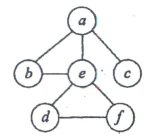
\includegraphics[width=0.3\textwidth]{../../figure/exercisePicPDF/chapter7/7-53.pdf}
            \caption{深度优先遍历}
            \label{fig:7-53}
    \end{figure}

        A. 5 个 \quad B. 4 个 \quad C. 3 个 \quad D. 2 个  
    
        \item 图\ref{fig:7-54}给出由 7 个顶点组成的无向图。从顶点 1 出发,对它进行深度优先遍历得到的序列是( );而进行广度优先遍历得到的顶点序列是( )。  
        【中科院软件所 1999 六、2(2 分)】  

        \begin{figure}[h!]
            \centering
            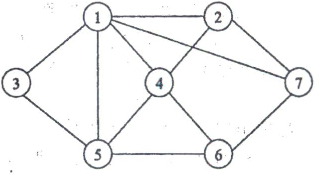
\includegraphics[width=0.3\textwidth]{../../figure/exercisePicPDF/chapter7/7-54.pdf}
            \caption{深度优先遍历}
            \label{fig:7-54}
    \end{figure}
        A. 深度优先:$1, 3, 5, 4, 2, 6, 7$;广度优先:$1, 5, 3, 4, 2, 6, 7$  

        B. 深度优先:$1, 3, 4, 7, 6, 5, 2$;广度优先:$1, 7, 2, 6, 4, 5, 3$  

        C. 深度优先:$1, 5, 3, 4, 2, 7, 6$;广度优先:$1, 3, 5, 4, 2, 7, 6$  

        D. 以上答案均不正确  
    
        \item 下面哪一方法可以判断出一个有向图是否有环(回路)?( )  
        【东北大学 2000 四、2(4 分)】  

        A. 深度优先遍历 \quad B. 拓扑排序 \quad C. 求最短路径 \quad D. 求关键路径  
    
        \item 判断有向图是否有回路,除了可以用拓扑排序外,还可以用( )。  
        【南京理工大学 2004 一、7(2 分)】  

        A. 求关键路径的算法  

        B. 广度优先遍历算法  

        C. 求最短路径的算法  

        D. 深度优先遍历算法  
    
        \item 用邻接表表示图进行深度优先遍历时,通常是采用( )来实现算法的。  
        【新疆大学 2017 二、8(2 分)】  

        A. 栈 \quad B. 队列 \quad C. 树 \quad D. 图  
    
        \item 在求边稠密的图的最小代价生成树时,采用( )算法较合适。  
        【上海交通大学 2005 四、7(2 分)】  
        
        A. 普里姆(Prim)  

        B. 克鲁斯卡尔(Kruskal)  

        C. 迪杰斯特拉(Dijkstra)  

        D. 其他  
    
        \item 在具有 $n$ 个顶点的图 $G$ 中,若最小生成树不唯一,则( )。  
        【电子科技大学 2008 一、2(2 分)】 

        A. $G$ 的边数一定大于 $n-1$  

        B. $G$ 的权值最小的边一定有多条  

        C. $G$ 的最小生成树的代价不一定相等  

        D. 以上选项都不对  

        \item 关于 Dijkstra 和 Floyd 算法的叙述中,不正确的是( )。  
    【南京理工大学 2000 一、21(1.5 分)】  

    1. 求从指定源点到其余各顶点的 Dijkstra 最短路径算法中弧上权不能为负的原因是在实际应用中无意义。  

    2. 利用 Dijkstra 求每一对不同顶点之间的最短路径的算法时间复杂度是 $O(n^2)$(图用邻接矩阵表示)。

    3. Floyd 求每对不同顶点对的算法中允许弧上的权为负,但不能有权和为负的回路。  

    A. 1 \quad B. 2 \quad C. 3 \quad D. 以上都不正确  

    \item 当各边上的权值( )时,Dijkstra 算法可以用来求解最短路径问题。  
    【中科院计算所 2000】  

    A. 均相等 \quad B. 均互不相等 \quad C. 不一定相等  

    \item 求解最短路径的 Floyd 算法的时间复杂度为( )。  
    【合肥工业大学 1999 二、2(2 分);中南大学 2005 一、8(2 分)】  

    A. $O(n)$ \quad B. $O(n+e)$ \quad C. $O(n^2)$ \quad D. $O(n^3)$  

    \item 已知有向图 $G = (V, E)$,其中  
    $V = \{V_1, V_2, V_3, V_4, V_5, V_6, V_7\}$,  
    $E = \{( V_1, V_2) ,  (V_1, V_3) ,  (V_1, V_4) ,  (V_2, V_5) ,  
    (V_3, V_5 ),  (V_3, V_6) ,  (V_4, V_6),  (V_5, V_7),  (V_6, V_7) \}$。  

    $G$ 的拓扑序列是( )。  
    【北京航空航天大学 2000 一、7(2 分)】  

    \begin{enumerate}[A.]
        \item $V_1, V_3, V_4, V_6, V_2, V_5, V_7$
        \item $V_1, V_3, V_2, V_6, V_4, V_5, V_7$
        \item $V_1, V_3, V_4, V_5, V_2, V_6, V_7$
        \item $V_1, V_2, V_5, V_3, V_4, V_6, V_7$
    \end{enumerate}

    \item 若一个有向图的邻接矩阵中主对角线以下的元素均为零,则该图的拓扑有序序列( )。  
    【中科院计算所 1998 二、6(2 分);中国科技大学 1998 二、6(2 分)】  

    A. 存在 \quad B. 不存在  

    \item 在有向图 $G$ 的拓扑序列中,若顶点 $u$ 在顶点 $v$ 之前,则下列情形不可能出现的是( )。  
    【江苏大学 2006 一、1(2 分)】  

    A. $G$ 中存在弧 $(u, v)$  

    B. $G$ 中不存在弧 $(u, v)$  

    C. $G$ 中存在一条从 $u$ 到 $v$ 的路径  

    D. $G$ 中存在一条从 $v$ 到 $u$ 的路径  

    \item 用邻接表表示图时,拓扑排序算法时间复杂度为( )。  
    【合肥工业大学 2000 一、2(2 分);南京理工大学 2001 一、9(1.5 分);青岛大学 2002 二、3(2 分)】 

    A. $O(n)$ \quad B. $O(n+e)$ \quad C. $O(n*e)$ \quad D. $O(n^2)$  

    \item 在下列网中,( )是边不带权值的图。  
    【华南理工大学 2007】  

    A. 邮电图 \quad B. AOV 网 \quad C. 公路网 \quad D. AOE 网  

    \item 关键路径是 AOE 网中( )。  
    【中南大学 2003 一、10(1 分)】  

    A. 从始点到终点的最短路径  

    B. 从始点到终点的最长路径  

    C. 从始点到终点的边数最多的路径  

    D. 从始点到终点的边数最少的路径  

    \item 下面关于求关键路径的说法不正确的是( )。  
    【南京理工大学 1998 一、12(2 分)】  

    A. 求关键路径是以拓扑排序为基础的  

    B. 一个事件的最早开始时间等于以该事件为尾的活动的最迟开始时间  

    C. 一个活动的总时差等于该活动的最迟开始时间减去最早开始时间  

    D. 关键活动一定位于关键路径上  

    \item 下列关于 AOE 网的叙述中,不正确的是( )。  
    【北京大学 2016 一、8(2 分);北京工业大学 1999 一、1(2 分);哈尔滨工业大学 2004 二、3(1 分)】  

    A. 关键活动不按期完成就会影响整个工程的完成时间  

    B. 任何一个关键活动提前完成,那么整个工程将会提前完成  

    C. 所有的关键活动提前完成,那么整个工程将会提前完成  

    D. 某些关键活动若提前完成,那么整个工程将会提前完成  

    \item 下列有关图的说法错误的是( )。  
    【中南大学 2003 二、19(1 分)】  

    A. 在有向图中,出度为 0 的结点称为叶子  

    B. 用邻接矩阵表示图容易判断任意两个结点之间是否有边相连,并求得各结点的度  

    C. 按深度方向遍历图和按先根次序遍历树类似,得到的结果是唯一的  

    D. 若有向图 $G$ 中从结点 $u$ 到结点 $v$ 有一条路径,则在图 $G$ 的结点的线性序列中结点 $u$ 必在结点 $v$ 之前  

    \item 下面的叙述中,不正确的是( )。  
    【吉林大学 2017 一、4(2 分)】  

    A. 任何一个关键活动不按期完成,就会影响整个工程的完成时间  

    B. 任何一个关键活动提前完成,将使整个工程提前完成  

    C. 所有关键活动都提前完成,将使整个工程提前完成  

    D. 所有关键活动不按期完成,就会影响整个工程的完成时间  

    \item 采用邻接表存储的图的深度优先遍历算法类似二叉树的( )算法。  
    【北京大学 2015 一、6(1.5 分)】  

    A. 前序遍历 \quad B. 中序遍历 \quad C. 后序遍历 \quad D. 按层次遍历  

    \item 在一个无向图中,所有顶点的度之和等于边之和的( )倍。  
    【北京大学 2016 一、7(2 分)】  

    A. $\frac{1}{2}$ \quad B. 1 \quad C. 2 \quad D. 4  

    \item 在一个有向图中,所有顶点的度数之和与图的边数的比是( )。  
    【烟台大学 2019 一、15(2 分)】  

    A. 1:2 \quad B. 1:1 \quad C. 2:1 \quad D. 4:1  

    \item 在一个包含 $n$ 个顶点的有向图中,如果所有顶点的出度之和为 $s$,则所有顶点的入度之和为( )。  
    【北京工业大学 2017 一、8(2 分)】  

    A. $n$ \quad B. $s$ \quad C. $2n$ \quad D. $s-1$  

    \item 若 $G$ 是一个具有 36 条边的非连通无向图(不含回路和多重边),则图 $G$ 的结点数至少是( )。  
    【北京大学 2015 一、7(1.5 分)】 

    A. 8 \quad B. 11 \quad C. 10 \quad D. 9  
\end{enumerate}

\chapter{树与散列}


\begin{enumerate}
    \item 在任意一棵非空平衡二叉树(AVL 树)$T_1$ 中,删除某结点 $w$ 之后形成平衡二叉树 $T_2$,再将 $w$ 插入 $T_2$ 形成平衡二叉树 $T_3$。下列关于 $T_1$ 与 $T_3$ 的叙述中,正确的是( )。  
    【2019 年全国试题 4(2 分)】  

    I. 若 $w$ 是 $T_1$ 的叶结点,则 $T_1$ 与 $T_3$ 可能不相同  

    II. 若 $w$ 不是 $T_1$ 的叶结点,则 $T_1$ 与 $T_3$ 一定不相同  

    III. 若 $w$ 不是 $T_1$ 的叶结点,则 $T_2$ 与 $T_3$ 一定相同  

    A. 仅 I \quad B. 仅 II \quad C. 仅 I、II \quad D. 仅 II、III  

    \item 现有长度为 11 且初始为空的散列表 $HT$,散列函数为 $h(\text{key}) = \text{key} \% 7$,采用线性探测再散列法解决冲突。将关键字序列 $88, 40, 30, 6, 11, 22, 98, 20$ 依次插入到 $HT$ 后,$HT$ 查找失败的平均查找长度是( )。  
    【2019 年全国试题 8(2 分)】  

    A. 4 \quad B. 5.25 \quad C. 6 \quad D. 6.29  

    \item 已知二叉排序树如图\ref{fig:9-3}所示,元素之间应满足的大小关系是( )。  
    【2018 年全国试题 6(2 分)】  

    \begin{figure}[h!]
        \centering
        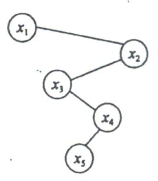
\includegraphics[width=0.3\textwidth]{../../figure/exercisePicPDF/chapter9/9-3.pdf}
        \caption{二叉排序树}
        \label{fig:9-3}
    \end{figure}
    A. $x_1 < x_2 < x_5$ 

    B. $x_1 < x_4 < x_5$  

    C. $x_3 < x_5 < x_4$  

    D. $x_4 < x_3 < x_5$  

    \item 高度为 5 的 3 阶 B 树含有的关键字个数至少是( )。  
    【2018 年全国试题 8(2 分)】  

    A. 15 \quad B. 31 \quad C. 62 \quad D. 242  

    \item 现有长度为 7、初始为空的散列表 $HT$,散列函数为 $h(k) = k \% 7$,用线性探测再散列法解决冲突。将关键字 $22, 43, 15$ 依次插入到 $HT$ 后,查找成功的平均查找长度是( )。  
    【2018 年全国试题 9(2 分)】  

    A. 1.5 \quad B. 1.6 \quad C. 2 \quad D. 3  

    \item 下列二叉树中,可能成为折半查找判定树(不含外部结点)的是( )。  
    【2017 年全国试题 8(2 分)】  

    \begin{figure}[h!]
        \centering
        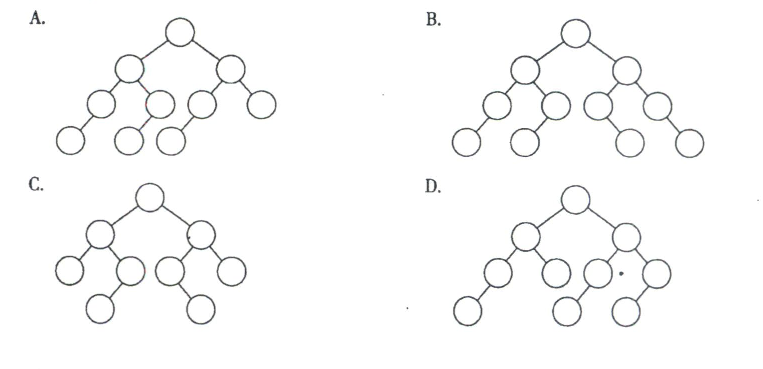
\includegraphics[width=0.8\textwidth]{../../figure/exercisePicPDF/chapter9/9-6.pdf}
        \caption{折半查找判定树}
    \end{figure}

    \item 下列应用中,适合使用 B+ 树的是( )。  
    【2017 年全国试题 9(2 分)】 

    A. 编译器中的词法分析  

    B. 关系数据库系统中的索引  

    C. 网络中的路由表快速查找  

    D. 操作系统的磁盘空闲块管理  

    \item 在有 $n$($n > 1000$)个元素的升序数组 $A$ 中查找关键字 $x$,查找算法的伪代码如下所示:  
    \begin{verbatim}
    k = 0;
    while (k < n 且 A[k] < x) k = k + 3;
    if (k < n 且 A[k] == x) 查找成功;
    else if (k - 1 < n 且 A[k - 1] == x) 查找成功;
        else if (k - 2 < n 且 A[k - 2] == x) 查找成功;
            else 查找失败;
    \end{verbatim}
    本算法与折半查找算法相比,有可能具有更少比较次数的情形是( )。  
    【2016 年全国试题 9(2 分)】  

    A. 当 $x$ 不在数组中  

    B. 当 $x$ 接近数组开头处  

    C. 当 $x$ 接近数组结尾处 

    D. 当 $x$ 位于数组中间位置  

    \item B+ 树不同于 B 树的特点之一是( )。  
    【2016 年全国试题 10(2 分)】  

    A. 能支持顺序查找  

    B. 结点中含有关键字  

    C. 根结点至少有两个分支  

    D. 所有叶结点都在同一层上  


    \item 假设顺序表中包含 5 个数据元素 $\{a, b, c, d, e\}$,它们的查找概率分别为 $0.3, 0.35, 0.2, 0.1, 0.05$,顺序查找时为了使查找成功的平均查找长度达到最小,则表中数据元素的存放顺序是( )。  
    【北京工业大学 2018 一、4(2 分)】  

    A. $\{e, d, c, b, a\}$  

    B. $\{b, a, c, d, e\}$
     
    C. $\{b, a, d, c, e\}$  

    D. $\{a, d, e, c, b\}$  

    \item 下列二叉排序树中,满足平衡二叉树定义的是( )。  
    【2009 年全国试题 4(2 分)】  

    \begin{figure}[h!]
        \centering
        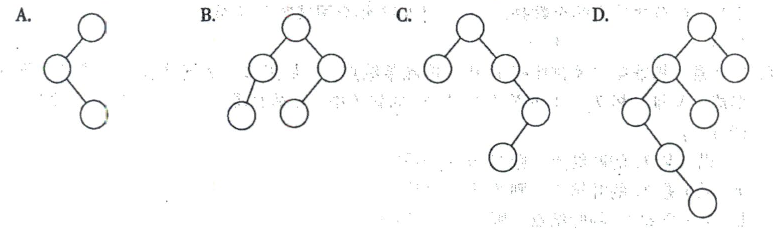
\includegraphics[width=0.6\textwidth]{../../figure/exercisePicPDF/chapter9/9-11.pdf}
        \caption{平衡二叉树}
        \label{fig:9-11}
    \end{figure}

    \item 下列叙述中,不符合m阶 B 树定义要求的是( )。  
    【2009 年全国试题 8(2 分)】 

    A. 根结点最多有m棵子树  

    B. 所有叶结点都在同一层上  

    C. 各结点内关键字均升序或降序排列  

    D. 叶结点之间通过指针链接  

    \item 在图\ref{fig:9-13}所示的平衡二叉树中,插入关键字 48 后得到一棵新平衡二叉树。在新平衡二叉树中,关键字 37 所在结点的左、右子结点中保存的关键字分别是( )。  
    【2010 年全国试题 4(2 分)】

    \begin{figure}[h!]
        \centering
        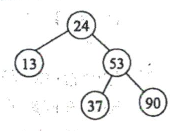
\includegraphics[width=0.4\textwidth]{../../figure/exercisePicPDF/chapter9/9-13.pdf}
        \caption{平衡二叉树}
        \label{fig:9-13}
    \end{figure}

    A. 13、48  

    B. 24、48  

    C. 24、53  

    D. 24、90  

    \item 已知一个长度为 16 的顺序表,其元素按关键字有序排列。若采用折半查找法查找其中不存在的元素,则关键字的比较次数最多是( )。  
    【2010 年全国试题 9(2 分)】  

    A. 4 \quad B. 5 \quad C. 6 \quad D. 7  

    \item 对于下列关键字序列,不可能构成某二叉排序树中一条查找路径的序列是( )。  
    【2011 年全国试题 7(2 分)】  

    A. $95, 22, 91, 24, 94, 71$ 

    B. $92, 20, 91, 34, 88, 35$  

    C. $21, 89, 77, 29, 36, 38$  

    D. $12, 25, 71, 68, 33, 24$  

    \item 为提高散列(Hash)表的查找效率,可以采取的正确措施是( )。  
    【2011 年全国试题 9(2 分)】  

    I. 增大装填(载)因子  

    II. 设计冲突(碰撞)少的散列函数  

    III. 处理冲突(碰撞)时避免产生堆积现象 

    A. 仅 I \quad B. 仅 II \quad C. 仅 II、III \quad D. 仅 I、III  

    \item 若平衡二叉树的高度为 6,且所有非叶结点的平衡因子均为 1,则该平衡二叉树的结点总数为( )。  
    【2012 年全国试题 4(2 分)】  

    A. 12 \quad B. 20 \quad C. 32 \quad D. 33  

    \item 设有一棵 3 阶 B 树,如下图\ref{fig:9-18}所示。删除关键字 78 得到一棵新 B 树,其最右叶结点所含的关键字是( )。  
    【2012 年全国试题 9(2 分)】  

    \begin{figure}[h!]
        \centering
        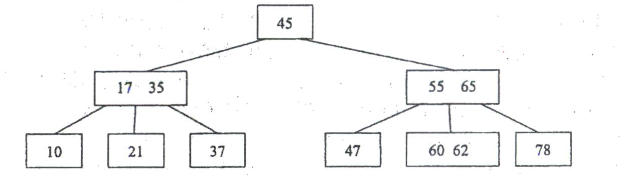
\includegraphics[width=0.8\textwidth]{../../figure/exercisePicPDF/chapter9/9-18.pdf}
        \caption{3 阶 B 树}
        \label{fig:9-18}
    \end{figure}

    A. 60 \quad B. $60, 62$ \quad C. $62, 65$ \quad D. 65  

    \item 若将关键字 $1, 2, 3, 4, 5, 6, 7$ 依次插入到初始为空的平衡二叉树 $T$ 中,则 $T$ 中平衡因子为 0 的分支结点的个数是( )。  
    【2013 年全国试题 3(2 分)】 

    A. 0 \quad B. 1 \quad C. 2 \quad D. 3  

    \item 在任意一棵非空二叉排序树 $T_1$ 中,删除某结点 $w$ 之后形成二叉排序树 $T_2$,再将 $w$ 插入 $T_2$ 形成二叉排序树 $T_3$。下列关于 $T_2$ 与 $T_3$ 的叙述中,正确的是( )。  
    【2013 年全国试题 6(2 分)】  

    I. 若 $w$ 是 $T_1$ 的叶结点,则 $T_2$ 与 $T_3$ 不同 

    II. 若 $w$ 是 $T_1$ 的叶结点,则 $T_2$ 与 $T_3$ 相同  

    III. 若 $w$ 不是 $T_1$ 的叶结点,则 $T_2$ 与 $T_3$ 不同 

    IV. 若 $w$ 不是 $T_1$ 的叶结点,则 $T_2$ 与 $T_3$ 相同  

    A. 仅 II、III \quad B. 仅 I、II \quad C. 仅 II、IV \quad D. 仅 I、III  

    \item 在一棵高度为 2 的 5 阶 B 树中,所含关键字的个数最少是( )。  
    【2013 年全国试题 10(2 分)】  

    A. 5 \quad B. 7 \quad C. 8 \quad D. 14  

    \item 用哈希(散列)方法处理冲突(碰撞)时可能出现堆积(聚集)现象。下列选项中,会受堆积现象直接影响的是( )。  
    【2014 年全国试题 8(2 分)】  

    A. 存储效率 \quad B. 散列函数 \quad C. 装填(装载)因子 \quad D. 平均查找长度  

    \item 在一棵具有 15 个关键字的 4 阶 B 树中,含关键字的结点数最多是( )。  
    【2014 年全国试题 9(2 分)】  

    A. 5 \quad B. 6 \quad C. 10 \quad D. 15  

    \item 现在有一棵无重复关键字的平衡二叉树(AVL 树),对其进行中序遍历可得到一个降序序列。下列关于该平衡二叉树的叙述中,正确的是( )。  
    【2015 年全国试题 4(2 分)】  

    A. 根结点的度一定为 2  

    B. 树中最小元素一定是叶结点  

    C. 最后插入的元素一定是叶结点  

    D. 树中最大元素一定是无左子树  

    \item 下列选项中,不能构成折半查找中关键字比较序列的是( )。  
    【2015 年全国试题 7(2 分)】  

    A. $500, 200, 450, 180$  

    B. $500, 450, 200, 180$  

    C. $180, 500, 200, 450$  

    D. $180, 200, 500, 450$  

    \item 若查找每个记录的概率均等,则在具有 $n$ 个记录的连续顺序文件中采用顺序查找法查找一个记录,其平均查找长度 ASL 为( )。  
    【北京航空航天大学 2000 一、8(2 分);大连理工大学 2008 一、5(2 分)】  

    A. $\frac{n-1}{2}$ \quad B. $\frac{n}{2}$ \quad C. $\frac{n+1}{2}$ \quad D. $n$  

    \item 对于顺序查找,假定查找成功与不成功的可能性相同,对每个记录的查找概率也相同,此时顺序查找的平均查找长度为( )。  
    【华中科技大学 2006 一、10(2 分)】  

    A. $0.5(n+1)$ \quad B. $0.25(n+1)$ \quad C. $0.5(n-1)$ \quad D. $0.75(n+1)$  

    \item 在一个有 $n$ 个元素的有序单链表中查找具有给定关键字的结点,平均情况下的时间复杂性为( )。  
    【上海交通大学 2005 四、2(2 分)】 

    A. $O(1)$ \quad B. $O(n)$ \quad C. $O(n^2)$ \quad D. $O(n \log n)$  

    \item 将两个各有 $n$ 个元素的有序表归并成一个有序表,其最多的比较次数是( )。  
    【中国科学技术大学 1998 二、9(2 分)】

    A. $2n$ \quad B. $n$ \quad C. $2n-1$

    \item 查找 $n$ 个元素的有序表时,最有效的查找方法是( )。  
    【中国科学技术大学 1997 一、1(1 分);四川大学 2005】  

    A. 顺序查找 \quad B. 分块查找 \quad C. 二分查找 \quad D. 二叉排序树  

    \item 对线性表进行二分查找时,要求线性表必须( )。  
    【南京理工大学 2005 一、11(1 分);中山大学 2001 一、5(2 分)】  

    A. 以顺序方式存储  

    B. 以顺序方式存储,且数据元素有序  

    C. 以链接方式存储  

    D. 以链接方式存储,且数据元素有序  

    \item 当在一个有序的顺序存储表上查找一个数据时,既可用折半查找,也可用顺序查找,但前者比后者的查找速度( )。  
    【南京理工大学 1997 一、7(2 分)】  

    A. 必定快  

    B. 不一定  

    C. 在大部分情况下要快  

    D. 取决于表递增还是递减  

    \item 一个有序表为 $\{1, 3, 9, 12, 32, 41, 45, 62, 75, 77, 82, 95, 100\}$,当二分查找值为 82 的结点时,( )次比较后查找成功。  
    【吉林大学 2016 一、5(2 分)】  

    A. 1 \quad B. 2 \quad C. 4 \quad D. 8  

    \item 折半查找有序表 $\{5, 8, 10, 22, 36, 50, 53, 88\}$,若查找元素 70,则需依次与表中元素(关键字)( )进行比较,查找结果是“失败”。  
    【华中科技大学 2006 一、11(2 分)】  

    A. $36, 53$  

    B. $22, 50, 53, 88$  

    C. $36, 53, 88$  

    D. $22, 53, 88$  

    \item 具有 12 个关键字的有序表,折半查找的平均查找长度是( )。  
    【中山大学 1998 二、10(2 分);烟台大学 2007 一、17(2 分)】  

    A. 3.1 \quad B. 4 \quad C. 2.5 \quad D. 5  

    \item 对一个长度为 50 的有序表进行折半查找,最多比较( )次就能查找出结果。  
    【西安交通大学 2005 一、8(2 分)】  

    A. 6 \quad B. 7 \quad C. 8 \quad D. 9  

    \item 折半查找有序表 $\{2, 10, 25, 35, 40, 65, 70, 75, 81, 82, 88, 100\}$,若查找元素 75,需要依次与表中元素( )进行比较。  
    【华中科技大学 2007 一、5(2 分)】  

    A. $65, 82, 75$  

    B. $70, 82, 75$  

    C. $65, 81, 75$  

    D. $65, 81, 70, 75$  

    \item 折半查找的时间复杂度为( )。  
    【中山大学 1999 一、15(2 分)】  

    A. $O(n^2)$ \quad B. $O(n)$ \quad C. $O(n \log n)$ \quad D. $O(\log n)$  

    \item 当采用分块查找时,数据的组织方式为( )。  
    【南京理工大学 1996 一、7(2 分)】  

    A. 数据分成若干块,每块内数据有序  

    B. 数据分成若干块,每块内数据不必有序,但块间必须有序,每块内最大(或最小)的数据组成索引块  

    C. 数据分成若干块,每块内数据有序,每块内最大(或最小)的数据组成索引块  

    D. 数据分成若干块,每块(除最后一块外)中数据个数需相同  

    \item 对表长为 $n$ 的有序表进行折半查找,其判定树高度为( )。  
    【北京交通大学 2004 一、8(2 分)】  

    A. $\lceil \log_2(n+1) \rceil$  

    B. $\lfloor \log_2(n+1) \rfloor$  

    C. $\lceil \log_2 n \rceil$  

    D. $\lfloor \log_2 n \rfloor$  

    \item 顺序查找法适合于存储结构为( )的线性表。  
    【北京航空航天大学 2002】  

    A. 顺序存储结构或链式存储结构 

    B. 散列存储结构  

    C. 索引存储结构  


    D. 压缩存储结构  

    \item 对大小均为 $n$ 的有序表和无序表分别进行顺序查找,在等概率查找的情况下,对于查找失败,它们的平均查找长度是( 1 );对于查找成功,它们的平均查找长度是( 2 )。  
    【上海海事大学 1997 二、4(3 分)】  

    A. 相同的 \quad B. 不同的  

    \item 在下列查找方法中,平均查找速度最快的是( )。  
    【四川大学 2005】  

    A. 顺序查找 \quad B. 折半查找 \quad C. 分块查找 \quad D. 二叉排序树查找  

    \item 如果要求一个线性表既能较快地查找,又能适应动态变化的要求,可以采用下列( )查找方法。  
    【北京交通大学 2005 一、3(2 分)】  

    A. 分块查找 \quad B. 顺序查找 \quad C. 折半查找 \quad D. 哈希查找  

    \item 当 $n$ 足够大时,在按值有序的顺序表中进行折半查找,在查找概率相等的情况下,其查找成功的平均查找长度是( )。  
    【北京航空航天大学 2002】  

    A. $\frac{n+1}{2}$ \quad B. $\frac{n}{2}$ \quad C. $\log_2(n+1) - 1$ \quad D. $\log_2(n+1)$  

    \item 在下述几种树中,( )可以表示静态查找表。  
    【中国科学技术大学 1995 十四、10(2 分)】  

    A. 次优查找树 \quad B. 二叉排序树 \quad C. B-树 \quad D. 平衡二叉树  

    \item 以下说法正确的是( )。  
    【北京交通大学 2006 一、4(2 分)】  

    A. 先序遍历二叉排序树的结点就可以得到排好序的结点序列 

    B. 任一二叉排序树的平均查找时间都小于顺序查找法查找同样结点的线性表的平均查找时间  

    C. 对具有相同关键字集合的任一插入序列,得到的二叉排序树的形态都是相同的  

    D. 采用分块查找方法,既能实现较快地查找线性表,又能适应动态变化的要求  

    \item 折半查找过程所对应的判定树是一棵( )。  
    【北京交通大学 2007】  

    A. 最小生成树 \quad B. 平衡二叉树 \quad C. 完全二叉树 \quad D. 哈夫曼树  

    \item 对于二叉排序树,下面的说法( )是正确的。  
    【华南理工大学 2006 一、5(2 分)】  

    A. 二叉排序树是动态树表,查找不成功时插入新结点会引起树的重新分裂和组合  

    B. 对二叉排序树进行层序遍历可得到有序序列  

    C. 用逐点插入法构造二叉排序树时,若先后插入的关键字有序,二叉排序树的深度最大  

    D. 在二叉排序树中进行查找,关键字的比较次数不超过结点数的 1/2  

    \item 对动态查找有高效率的查找表组织结构是( )。  
    【哈尔滨工程大学 2005】  

    A. 有序表 \quad B. 分块有序表 \quad C. 循环链表 \quad D. B-树  

    \item 下列二叉排序树中查找效率最高的是( )。  
    【中南大学 2003 二、11(1 分)】  

    A. 平衡二叉树 \quad B. 二叉查找树 \quad C. 没有左子树的二叉排序树 \quad D. 没有右子树的二叉排序树  

    \item 构造一棵具有 $n$ 个结点的二叉排序树,最理想情况下的深度为( )。  
    【华中科技大学 2007 一、14(2 分)】 

    A. $n/2$ \quad B. $n$ \quad C. $\lfloor \log_2(n+1) \rfloor$ \quad   D. $\lceil \log_2(n+1) \rceil$ 

    \item 设二叉排序树中关键字由 1 到 1000 的整数构成,现要查找关键字为 363 的结点,下述关键字序列中,不可能是在查找过程中访问的序列是( )。  
    【北京交通大学 2005 一、1(2 分)】  

    A. $2, 252, 401, 398, 330, 344, 397, 363$  

    B. $924, 220, 911, 244, 898, 258, 363$  

    C. $925, 202, 911, 240, 912, 245, 363$  

    D. $2, 399, 387, 219, 266, 382, 381, 278, 363$  

    \item 分别以下列序列构造二叉排序树,与其他三个结果不同的是( )。  
    【合肥工业大学 2000 一、4(2 分)】 

    A. $100, 80, 90, 60, 120, 110, 130$  

    B. $100, 120, 110, 130, 80, 60, 90$  

    C. $100, 60, 80, 90, 20, 110, 130$  

    D. $100, 80, 60, 90, 120, 130, 110$  

    \item 分别以下列序列构造二叉排序树,与众不同的是( )。  
    【中国科学技术大学 2004】  

    A. $100, 80, 60, 85, 110, 120, 150$  

    B. $100, 80, 60, 85, 120, 110, 150$  

    C. $100, 80, 85, 60, 120, 110, 150$  

    D. $100, 80, 60, 85, 120, 150, 110$  

    \item 在平衡二叉树中插入一个结点后造成了不平衡,设最低的不平衡结点为 $A$,并已知 $A$ 的左孩子的平衡因子为 0,右孩子的平衡因子为 1,则应作( )型调整以使其平衡。  
    【合肥工业大学 2001 一、4(2 分)】  

    A. LL \quad B. LR \quad C. RL \quad D. RR  

    \item 设输入序列为 $120, 35, \dots$,构造一棵平衡二叉树,当在树中插入值 30 时发生不平衡,则应进行的平衡旋转是( )。  
    【南京理工大学 2005 一、4(1 分)】  

    A. LL \quad B. RL \quad C. LR \quad D. RR  

    \item 已知一棵深度为 $h$ 的平衡二叉树,其每个非叶子结点的平衡因子均为 0,则该树共有结点总数为( )。  
    【北京交通大学 2006 一、2(2 分)】  

    A. $2^{h-1} - 1$ \quad B. $2^{h-1} + 1$ \quad C. $2^{h} - 1$ \quad D. $2^{h} + 1$  

    \item 在平衡二叉树中,进行查找的效率与( )有关。  
    【北京航空航天大学 2004】  

    A. 二叉树的深度  

    B. 二叉排序树的结点的个数  

    C. 后序线索树  

    D. 所有线索树  

    \item 下列关于 $m$ 阶 B 树的说法错误的是( )。  
    【南京理工大学 1997 一、9(2 分)】  

    A. 根结点至多有 $m$ 棵子树  

    B. 所有叶子都在同一层次上  

    C. 非叶结点至少有 $\lceil m/2 \rceil$ 棵子树  

    D. 根结点中的数据是有序的  

    \item 下面关于 $m$ 阶 B 树的说法正确的是( )。  
    【南京理工大学 1999 一、5(2 分)】  

    A. 每个结点至少有两棵非空子树  

    B. 树中每个结点至多有 $m-1$ 个关键字  

    C. 所有叶子在同一层上  

    D. 当插入一个数据项引起 B 树结点分裂后,树长高一层  

    \item 下面关于 B 树和 B+ 树的叙述中,不正确的是( )。  
    【北方交通大学 2001 一、17(2 分)】  

    A. B 树和 B+ 树都是平衡的多路树  

    B. B 树和 B+ 树都可用于文件的索引结构  

    C. B 树和 B+ 树都能有效地支持顺序检索  


    D. B 树和 B+ 树都能有效地支持随机检索  

    \item $m$ 阶 B 树是一棵( )。  
    【北京大学 2015 一、9(1.5 分)】  

    A. $m$叉排序树  

    B. $m$ 路平衡排序树  

    C. $m-1$ 路平衡排序树  

    D. $m+1$ 路平衡排序树  

    \item 在一棵含有 $n$ 个关键字的 $m$ 阶 B 树中进行查找,至多读盘( )次。  
    【中科院计算所 2000 一、6(2 分)】 

    A. $\log n$ \quad B. $1 + \log n$ \quad C. $1 + \log_{\lceil m/2 \rceil} \frac{n+1}{2}$ \quad D. $1 + \log_{\lceil n/2 \rceil} \frac{m+1}{2}$  

    \item $m$ 阶 B+ 树是一棵( 1 ),其结点中关键字最多为( 2 )个,最少为( 3 )个。  
    【中科院计算所 1999 一、5(6 分)】  

    A. $m$ 路平衡查找树 \quad B. $m$ 路平衡索引树 \quad C. $m$ 路 Ptrie 树 \quad D. $m$ 路键树  

    E. $m-1$ \quad F. $m$ \quad G. $m+1$ \quad H. $\lceil m/2 - 1 \rceil$  \quad I. $\lceil m/2 \rceil$ \quad J. $\lceil m/2 + 1 \rceil$

    \item 一棵 3 阶 B 树中含有 2047 个关键字,包括叶子结点层,该树的最大深度为( )。  
    【北京交通大学 2005 一、2(2 分)】  

    A. 11 \quad B. 12 \quad C. 13 \quad D. 14  

    \item 已知一棵 5 阶 B 树有 53 个关键字,并且每个结点的关键字都达到最少状态,则它的深度是( )。  
    【华南理工大学 2006 一、8(2 分)】  

    A. 3 \quad B. 4 \quad C. 5 \quad D. 6  

    \item B+ 树是( )。  
    【武汉理工大学 2004 一、13(3 分)】  

    A. 一种 AVL 树  

    B. 索引表的一种组织形式  

    C. 一种高度不小于 1 的树  

    D. 一种与二进制有关的树  

    \item 当向 B 树插入关键字时,可能引起结点的( ),最终可能导致整个 B 树的高度( )。  
    【浙江大学 2004】  

    A. 合并 \quad B. 增加 1 \quad C. 分裂 \quad D. 减少 1  

    \item 在一棵 $m$ 阶 B 树中,若在某结点中插入一个新关键字而引起该结点的分裂,则此结点中原有的关键字个数是( )。  
    【湖南大学 2003】 

    A. $m$ \quad B. $m+1$ \quad C. $m-1$ \quad D. $m/2$  

    \item 含有 $n$ 个非叶子结点的 $m$ 阶 B 树至少包含( )个关键字。  
    【北京交通大学 2004】 

    A. $(m-1) \cdot n$ \quad B. $n$  \quad C. $n \cdot (m/2 - 1)$ \quad D. $(n-1) \cdot (m/2 - 1) + 1$

    \item 理论上,散列表的平均比较次数为( )次。  
    【北京邮电大学 2005 一、9(2 分)】  

    A. 1 \quad B. 2 \quad C. 4 \quad D. $n$  

    \item 散列函数有一个共同的性质,即函数值应当以( )取其值域的每个值。  
    【西安电子科技大学 2001 应用一、7(2 分);北京邮电大学 1999 一、4(2 分)】  

    A. 最大概率 \quad B. 最小概率 \quad C. 平均概率 \quad D. 同等概率  

    \item 将 10 个元素散列到 100,000 个单元的哈希表中,则( )产生冲突。  
    【北京邮电大学 2001 一、4(2 分)】  

    A. 一定会 \quad B. 一定不会 \quad C. 仍可能会  

    \item 采用链地址法解决冲突的哈希表中,查找成功的平均查找长度( )。  
    【北京交通大学 2005 一、6(2 分);2007】  

    A. 直接与关键字个数有关  

    B. 直接与装填因子有关  

    C. 直接与表的容量有关  

    D. 与冲突次数无关  

    \item 下面关于哈希(Hash)查找的说法正确的是( )。  
    【北京大学 1998 一、10(2 分);烟台大学 2007 一、18(2 分)】  

    A. 哈希函数构造得越复杂越好,因为这样随机性好  

    B. 除留余数法是所有哈希函数中最好的  

    C. 不存在特别好与坏的哈希函数,要视情况而定  

    D. 不管用何种方法解决冲突,只要简单地将该元素删除即可  

    \item 在构造哈希表方面,下面的说法是正确的( )。  
    【南理工大学 2005 一、4(2 分)】  

    A. 再散列在处理冲突时不会产生聚集  

    B. 散列表的装载因子越大,说明空间利用率越好,因此应尽量大  

    C. 散列函数选得好可减少冲突现象  

    D. 对于任何具体关键字都可能找到不产生冲突的散列函数  

    \item 散列文件的特点是( )。  
    【烟台大学 2007 一、20(2 分)】 

    A. 记录按照关键字排序  

    B. 记录可以顺序存取  

    C. 存取速度快,但占用的存储空间较多  

    D. 记录不需要排序,存取速度快  

    \item 若采用链地址法构造散列表,散列函数为 $h(\text{key}) = \text{key} \mod 17$,则需( 1 )个链表。这些链的链首指针构成一个指针数组,数组的下标范围为( 2 )。  
    【南京理工大学 1999 一、12(4 分)】 

    (1)  

    A. 17 \quad B. 13 \quad C. 16 \quad D. 任意  

    (2)  

    A. 0 至 17 \quad B. 1 至 17 \quad C. 0 至 16 \quad D. 1 至 16  

    \item 设有一组记录的关键字为 $\{19, 14, 23, 1, 68, 20, 84, 27, 55, 11, 10, 79\}$,用链地址法构造散列表,散列函数为 $h(\text{key}) = \text{key} \mod 13$,散列地址为 1 的链中有( )个记录。  
    【南京理工大学 1997 一、4(2 分)】  

    A. 1 \quad B. 2 \quad C. 3 \quad D. 4  

    \item 已知一个线性表 $\{1, 13, 12, 34, 38, 33, 27, 22\}$,假定采用 $h(k) = k \mod 11$ 计算散列地址进行散列存储,若用链地址法处理冲突,则查找成功的平均查找长度为( )。  
    【哈尔滨工业大学 2005 二、6(1 分)】  

    A. 1 \quad B. $9/8$ \quad C. $13/11$ \quad D. $13/8$  

    \item 设散列表长 $M = 14$,哈希函数 $h(\text{KEY}) = \text{KEY} \mod 11$。表中已有 4 个结点:  
    $\text{ADDR}(15) = 4$,$\text{ADDR}(38) = 5$,$\text{ADDR}(61) = 6$,$\text{ADDR}(84) = 7$,其余地址为空。如用二次探测再散列处理冲突,关键字为 49 的结点的地址是( )。  
    【东华大学 2001 一、8(1 分)】 

    A. 8 \quad B. 3 \quad C. 5 \quad D. 9  

    \item 假定有 $n$ 个关键字互为同义词,若用线性探测法把这 $n$ 个关键字存入散列表中,至少要进行多少次探测?( )  
    【中国科技大学 1998 二、3(2 分);中科院计算所 1998 二、3(2 分)】  

    A. $n-1$ 次 \quad B. $n$ 次 \quad C. $n+1$ 次 \quad D. $\frac{n(n+1)}{2}$ 次  

    \item 散列表的地址区间为 $0 \sim 17$,散列函数为 $h(K) = K \mod 17$。采用线性探测法处理冲突,并将关键字序列 $\{26, 25, 72, 38, 8, 18, 59\}$ 依次存储到散列表中:  
    
    (1) 元素 59 存放在散列表中的地址是( )。 

    A. 8 \quad B. 9 \quad C. 10 \quad D. 11  
   
    (2) 存放元素 59 需要搜索的次数是( )。  
   
    A. 2 \quad B. 3 \quad C. 4 \quad D. 5  
    【北方交通大学 2001 一(19,20)(4 分)】  

    \item 关于哈希查找,说法不正确的有( )个。  
    【南京理工大学 2000 一、16(1.5 分)】  

    (1) 采用链地址法解决冲突时,查找一个元素的时间是相同的  

    (2) 采用链地址法解决冲突时,若规定插入总是在链首,则插入和查找一个元素的时间是相同的  

    (3) 用链地址法解决冲突易引起聚集现象  

    (4) 再哈希法不易产生聚集  

    A. 1 \quad B. 2 \quad C. 3 \quad D. 4  

    \item 采用开地址法解决冲突的哈希查找中,发
    生聚集的原因主要是( )。  
    【中国科学技术大学 1997 一、4(1 分)】  

    A. 数据元素过多  

    B. 负载因子过大  

    C. 哈希函数选择不当  

    D. 解决冲突的算法选择不好  

    \item 在采用链地址法处理冲突所构成的散列表上查找某一关键字,在查找成功的情况下,所探测的这些位置上的键值( )。  
    【北京交通大学 2006 一、6(2 分)】  

    A. 一定都是同义词  

    B. 不一定都是同义词  

    C. 都相同  

    D. 一定都不是同义词  

    \item 查找低效的数据结构是( )。  
    【中国科学院 2006】  

    A. 有序顺序表  

    B. 二叉排序树  

    C. 堆  

    D. 平衡的二叉排序树  

    \item 假定关键字 $K = 2 789 465$,允许存储地址为 3 位十进制数,现在得到的散列地址为 149,则所采用的构建散列函数的方法是( )。  
    【南开大学 2005】  

    A. 除留余数法,模为 23  

    B. 平方取中法  

    C. 移位叠加法  

    D. 边界倒加法  
    \item 设散列地址空间为 $0 \sim m-1$,对关键字 $K$,用去除 $p$,将所得到的余数作为散列地址,即 $h(K) = K \mod p$。为了减少发生冲突的概率,一般取 $p$ 为( )。  
    【中国科学院自动化所】

    A. 小于 $m$ 的最大偶数  

    B. 小于 $m$ 的最大素数  

    C. $m$ 的平方根  

    D. 小于 $m$ 的最大整数  

    \item 哈希表构建时采用线性探测法处理冲突,在某关键字查找成功的情况下,所探测的多个位置上的关键字( )。  
    【北京工业大学 2018 一、7(2 分)】  

    A. 不一定都是同义词  

    B. 一定是同义词  

    C. 一定都不是同义词  

    D. 必然有序  

    \item 对有 18 个元素的有序表 $A$ 作二分(折半)查找,则查找 $A[3]$ 的比较序列的下标为( )。  
    【吉林大学 2017 一、5(2 分)】  

    A. $1, 2, 3$  

    B. $9, 5, 2, 3$  

    C. $9, 5, 3$  

    D. $9, 4, 2,3$  

\end{enumerate}

\chapter{排序}


\begin{enumerate}
    \item 选择一个排序算法时,除算法的时空效率外,下列因素中,还需要考虑的是( )。  
    【2019 年全国试题 7(2 分)】  

    I. 数据的规模  

    II. 数据的存储方式  

    III. 算法的稳定性  

    IV. 数据的初始状态  



    A. 仅 III \quad B. 仅 I、II \quad C. 仅 II、III、IV \quad D. I、II、III、IV

    \item 排序过程中,快速排序的“第二趟”结果。下列序列中,不可能是快速排序第二趟结果的是( )。  
    【2019 年全国试题 10(2 分)】  

    A. $5, 2, 16, 12, 28, 60, 32, 72$  

    B. $2, 16, 5, 28, 12, 60, 32, 72$ 

    C. $2, 12, 16, 5, 28, 32, 72, 60$  

    D. $5, 2, 12, 28, 16, 32, 72, 60$  

    \item 设外存上有 120 个初始归并段,进行 12 路归并时,为实现最佳归并,需要补充的虚段个数是( )。  
    【2019 年全国试题 11(2 分)】 

    A. 1 \quad B. 2 \quad C. 3 \quad D. 4  

    \item 对初始数据序列 $\{8, 3, 9, 11, 2, 1,4, 7, 5, 10, 6\}$ 进行希尔排序。若第一趟排序结果为 $\{1,3,7,5,2,6,4, 9, 11, 10, 8\}$,
    第二趟排序结果为 $\{1, 2, 6, 4, 3, 7, 5, 8,11, 10, 9\}$,则两趟排序采用的增量(间隔)依次是( )。  
    【2018 年全国试题 10(2 分)】 

    A. 3, 1 \quad B. 3, 2 \quad C. 5, 2 \quad D. 5, 3  

    \item 在将数据序列 $\{6, 1, 5, 9, 8, 4, 7\}$ 建成大根堆时,正确的序列变化过程是( )。  
    【2018 年全国试题 11(2 分)】

    \begin{enumerate}[A.]
    \item $6, 1, 7, 9, 8, 4, 5 \to 6, 9, 7, 1, 8, 4, 5 \to 9, 6, 7, 1, 8, 4, 5 \to 9, 8, 7, 1, 6, 4, 5$
    \item $6, 9, 5, 1, 8, 4, 7 \to 6, 9, 7, 1, 8, 4, 5 \to 9, 6, 7, 1, 8, 4, 5 \to 9, 8, 7, 1, 6, 4, 5$
    \item $6, 9, 5, 1, 8, 4, 7 \to 9, 6, 5, 1, 8, 4, 7 \to 9, 6, 7, 1, 8, 4, 5 \to 9, 8, 7, 1, 6, 4, 5$
    \item $6, 1, 7, 9, 8, 4, 5 \to 7, 1, 6, 9, 8, 4, 5 \to 7, 9, 6, 1, 8, 4, 5 \to 9, 8, 6, 1, 7, 4, 5$
    \end{enumerate}
    \item 在内部排序时,若选择了归并排序而没有选择插入排序,则可能的理由是( )。  
    【2017 年全国试题 10(2 分)】  

    I. 归并排序的程序代码更短  

    II. 归并排序占的空间更少  

    III. 归并排序的运行效率更高 

    A. 仅 II \quad B. 仅 III \quad C. 仅 I、II \quad D. 仅 I、III  

    \item 下列排序方法中,若将顺序存储更换为链式存储,有时则效率更高的是( )。  
    【2017 年全国试题 11(2 分)】  

    I. 插入排序  

    II. 选择排序  

    III. 冒泡排序  

    IV. 希尔排序  

    V. 堆排序  

    A. 仅 I、II \quad B. 仅 II、III \quad C. 仅 III、IV \quad D. 仅 IV、V  

    \item 对 10TB 的数据文件进行排序,应使用的方法是( )。  
    【2016 年全国试题 11(2 分)】  

    A. 希尔排序 \quad B. 堆排序 \quad C. 快速排序 \quad D. 归并排序  

    \item 下列排序算法中,( )每一趟都能选出一个元素放在其最终位置上,并且是不稳定的。  
    【北京大学 2016 一、9(2 分)】  

    A. 冒泡排序 \quad B. 希尔排序 \quad C. 简单选择排序 \quad D. 快速排序  

    \item 若一组记录的关键字为 $\{45, 80, 55, 40, 42, 85\}$,则利用堆排序方法建立的初始堆为( )。  
    【吉林大学 2017 一、2(2 分)】  

    A. $80, 45, 55, 40, 42, 85$  

    B. $85, 80, 55, 40, 42, 45$  

    C. $85, 80, 55, 45, 42, 40$  

    D. $85, 55, 80, 42, 45, 40$  

    \item 已知关键字序列 $\{5, 8, 12, 19, 28, 20, 15, 22\}$ 是小根堆(最小堆),插入关键字 3,调整后得到的小根堆是( )。  
    【2009 年全国试题 9(2 分)】  

    A. $3, 5, 12, 8, 28, 20, 15, 22, 19$  

    B. $3, 5, 12, 19, 20, 15, 22, 8, 28$  

    C. $3, 8, 12, 5, 20, 15, 22, 28, 19$  

    D. $3, 12, 5, 8, 28, 20, 15, 22, 19$  

    \item 若数据元素序列 $\{11, 12, 13, 7, 8, 9, 23, 4, 5\}$ 是采用下列排序方法之一得到的第二趟排序后的结果,则该排序算法只能是( )。  
    【2009 年全国试题 10(2 分)】  

    A. 冒泡排序 \quad B. 插入排序 \quad C. 选择排序 \quad D. 二路归并排序  

    \item 采用递归方式对顺序表进行快速排序。下列关于递归次数的叙述中,正确的是( )。  
    【2010 年全国试题 10(2 分)】  

    A. 递归次数与初始数据的排列次序无关  

    B. 每次划分后,先处理较长的分区可以减少递归次数  

    C. 每次划分后,先处理较短的分区可以减少递归次数  
    
    D. 递归次数与每次划分后得到的分区的处理顺序无关  

    \item 对一组数据 $\{2, 12, 16, 88, 5, 10\}$ 进行排序,若前三趟排序结果如下:  
    
    第一趟排序结果:$2, 12, 16, 5, 10, 88$  
    
    第二趟排序结果:$2, 12, 5, 10, 16, 88$  
    
    第三趟排序结果:$2, 5, 10, 12, 16, 88$  
   
    则采用的排序方法可能是( )。  
    【2010 年全国试题 11(2 分)】  

    A. 冒泡排序 \quad B. 希尔排序 \quad C. 归并排序 \quad D. 基数排序  

    \item 为实现快速排序算法,待排序序列宜采用的存储方式是( )。  
    【2011 年全国试题 10(2 分)】  

    A. 顺序存储 \quad B. 散列存储 \quad C. 链式存储 \quad D. 索引存储  

    \item 已知序列 $\{25, 13, 10, 12, 9\}$ 是大根堆,在序列尾部插入新元素 18,将其再调整为大根堆,调整过程中元素之间进行的比较次数是( )。  
    【2011 年全国试题 11(2 分)】  

    A. 1 \quad B. 2 \quad C. 4 \quad D. 5  

    \item 排序过程中,对尚未确定最终位置的所有元素进行一遍处理称为一趟排序。下列排序方法中,每一趟排序结束时都至少能够确定一个元素最终位置的方法是( )。  
    【2012 年全国试题 10(2 分)】  

    I. 简单选择排序  

    II. 希尔排序  

    III. 快速排序  

    IV. 堆排序  

    V. 二路归并排序  

    A. 仅 I、III、 IV \quad B. 仅 I、III、V \quad C. 仅 II、III、IV \quad D. 仅 III、IV、V  

    \item 对同一待排序序列分别进行折半插入排序和直接插入排序,两者之间可能的不同之处是( )。  
    【2012 年全国试题 11(2 分)】  

    A. 排序的总趟数  

    B. 元素的移动次数  

    C. 使用辅助空间的数量  

    D. 元素之间的比较次数

    \item 对给定的关键字序列 $\{110, 119, 007, 911, 114, 120, 122\}$ 进行基数排序,则第二趟分配收集后得到的关键字序列是( )。  
    【2013 年全国试题 11(2 分)】  

    A. $007, 110, 119, 114, 911, 120, 122$  

    B. $007, 110, 119, 114, 911, 122, 120$  

    C. $007, 110, 911, 114, 119, 120, 122$  

    D. $110, 120, 911, 122, 114, 007, 119$  

    \item 用希尔排序方法对一个数据序列进行排序时,若第一趟排序结果为 $\{9, 1, 4, 13, 7, 8, 20, 23, 15\}$,则该趟排序采用的增量(间隔)可能是( )。  
    【2014 年全国试题 10(2 分)】  

    A. 2 \quad B. 3 \quad C. 4 \quad D. 5  

    \item 下列选项中,不可能是快速排序第二趟排序结果的是( )。  
    【2014 年全国试题 11(2 分)】  

    A. $2,3, 5, 4,  6,7, 9$  

    B. $2,7,5,6,4,3,9$  

    C. $3, 2, 5,4, 7, 6, 9$  

    D. $4, 2, 3, 5, 7, 6, 9$  

    \item 下列排序算法中,元素的移动次数和关键字的初始排列次序无关的是( )。  
    【2015 年全国试题 9(2 分)】  

    A. 直接插入排序 \quad B. 冒泡排序 \quad C. 基数排序 \quad D. 快速排序  

    \item 已知小根堆为 $\{8, 15, 10, 21, 34, 16, 12\}$,删除关键字 8 之后需重建堆,在此过程中,关键字之间的比较次数是( )。  
    【2015 年全国试题 10(2 分)】  

    A. 1 \quad B. 2 \quad C. 3 \quad D. 4  

    \item 希尔排序的组内排序采用的是( )。  
    【2015 年全国试题 11(2 分)】 

    A. 直接插入排序 \quad B. 折半插入排序 \quad C. 快速排序 \quad D. 归并排序  

    \item 排序算法的稳定性是指( )。  
    【北京理工大学 2005 一、10(1 分)】  

    A. 经过排序之后,能使值相同的数据保持原顺序中的相对位置不变  

    B. 经过排序之后,能使值相同的数据保持原顺序中的绝对位置不变  

    C. 算法的排序性能与被排序元素的数量关系不大  

    D. 算法的排序性能与被排序元素的数量关系密切  

    \item 下面给出的四种排序法中,( )是稳定的排序方法。  
    【北京航空航天大学 1999 一、10(2 分)】 

    A. 插入排序 \quad B. 冒泡排序 \quad C. 二路归并排序 \quad D. 堆排序  

    \item 下列排序算法中,( )是稳定的。  
    【福州大学 1998 一、3(2 分)】  

    A. 堆排序,冒泡排序  

    B. 快速排序,堆排序  

    C. 直接选择排序,归并排序  

    D. 归并排序,冒泡排序  

    \item 稳定的排序方法是( )。  
    【北方交通大学 2000 二、3(2 分)】  

    A. 直接插入排序和快速排序  

    B. 折半插入排序和冒泡排序  

    C. 简单选择排序和四路归并排序  

    D. 树形选择排序和 Shell 排序  

    \item 下列排序方法中,哪一个是稳定的排序方法( )。  
    【北方交通大学 2001 一、8(2 分)】  

    A. 直接选择排序 \quad B. 二分法插入排序 \quad C. 希尔排序 \quad D. 快速排序  

    \item 下列排序算法中,( )是稳定排序。  
    【北京理工大学 2007 一、10(1 分)】  

    A. 希尔排序 \quad B. 快速排序 \quad C. 堆排序 \quad D. 直接插入排序  

    \item 如果待排序序列中两个数据元素具有相同的值,在排序前后它们的相互位置发生颠倒,则称该排序算法是不稳定的。( )就是不稳定的排序方法。  
    【清华大学 1998 一、3(2 分)】  

    A. 冒泡排序 \quad B. 归并排序 \quad C. Shell 排序 \quad D. 直接插入排序 \quad E. 简单选择排序  

    \item 若要求排序是稳定的,且关键字为实数,则在下列排序方法中应选( )排序为宜。  
    【中科院计算所 2000 一、5(2 分)】  

    A. 直接插入排序 \quad B. 直接选择排序 \quad C. 堆排序 \quad D. 快速排序 \quad E. 基数排序  

    \item 若需在 $O(n \log n)$ 的时间内完成对数组的排序,且要求排序是稳定的,则可选择的排序方法是( )。  
    【中国科技大学 1998 二、4(2 分);中科院计算所 1998 二、4(2 分)】  

    A. 快速排序 \quad B. 堆排序 \quad C. 归并排序 \quad D. 直接插入排序  

    \item 下面的排序算法中,不稳定的是( )。  
    【北京工业大学 1999 一、2(2 分)】  

    A. 冒泡排序 \quad B. 折半插入排序 \quad C. 简单选择排序 \quad D. 希尔排序  

    E. 基数排序 \quad F. 堆排序  

    \item 下列内部排序算法中:  
    \item 
    A. 快速排序 \quad B. 直接插入排序 \quad C. 二路归并排序 \quad D. 简单选择排序  

    E. 冒泡排序 \quad F. 堆排序  

    (1) 其比较次数与序列初态无关的算法是( )。 

    (2) 不稳定的排序算法是( )。  

    (3) 在初始序列已基本有序(除去 $k$ 个元素中的某 $k$ 个元素后即呈有序,$k < n$)的情况下,排序效率最高的算法是( )。  

    (4) 排序的平均时间复杂度为 $O(n \log n)$ 的算法是( ),为 $O(n^2)$ 的算法是( )。  

    【北京工业大学 2000 一、1(10 分,每问 2 分)】  

    \item 排序趟数与序列的原始状态有关的排序方法是( )排序法。  
    【北京航空航天大学 1999 一、5(2 分)】  

    A. 插入排序 \quad B. 选择排序 \quad C. 冒泡排序 \quad D. 快速排序  

    \item 下面给出的四种排序方法中,排序过程中的比较次数与排序方法无关的是( )。  
    【北京航空航天大学 2000 一、10(2 分)】

    A. 选择排序法 \quad B. 插入排序法 \quad C. 快速排序法 \quad D. 堆排序法  

    \item 排序方法中,关键字比较的次数与记录的初始排列无关的是( )。  
    【北京交通大学 2013 二、14(2 分)】  

    A. 简单选择排序 \quad B. 快速排序 \quad C. 直接插入排序 \quad D. Shell 排序  

    \item 对下列四种排序方法,在排序中关键字比较次数同记录初始排列无关的是( )。  
    【南京理工大学 2000 一、7(1.5 分)】  

    A. 直接插入排序 \quad B. 二分法插入排序 \quad C. 快速排序 \quad D. 归并排序  

    \item 在下列排序算法中,哪一个算法的时间复杂度与初始排序无关( )。  
    【北京理工大学 2001 六、4(2 分);北京工业大学 2005 一、4(2 分)】  

    A. 直接插入排序 \quad B. 冒泡排序 \quad C. 快速排序 \quad D. 直接选择排序  

    \item 下述几种排序方法中,要求内存量最大的是( )。  
    【中南大学 2005 一、6(2 分)】

    A. 归并排序 \quad B. 快速排序 \quad C. 插入排序 \quad D. 选择排序  

    \item 快速排序方法在( )情况下最不利于发挥其长处。  
    【华南理工大学 2007】  


    A. 要排序的数据量太大
     
    B. 要排序的数据中含有多个相同值  

    C. 要排序的数据个数为奇数  

    D. 要排序的数据已基本有序  

    \item 当待排序列基本有序时,下列排序方法中( )最好。  
    【北京邮电大学 2005 一、10(2 分)】  

    A. 直接插入排序 \quad B. 快速排序 \quad C. 堆排序 \quad D. 归并排序 

    \item 设被排序的结点序列共有 $N$ 个结点,在该序列中的结点已十分接近排序的情况下,用直接插入法、归并法和一般的快速排序法对其排序,这些算法的时间复杂性应为( )。  
    【上海交通大学 2005 四、5(2 分)】  

    A. $O(N)$,$O(N)$,$O(N)$  

    B. $O(N)$,$O(N \log N)$,$O(N \log N)$  

    C. $O(N)$,$O(N \log N)$,$O(N^2)$

    D. $O(N^2)$,$O(N^2 \log N)$,$O(N^2)$  

    \item 数据序列 $\{8, 9, 10, 4, 5, 6, 20, 1, 2\}$ 只能是下列排序算法中的( )的两趟排序后的结果。  
    【合肥工业大学 1999 一、3(2 分)】  

    A. 选择排序 \quad B. 冒泡排序 \quad C. 插入排序 \quad D. 堆排序  

    \item 一个排序算法的时间复杂度与( )有关。  
    【华中科技大学 2004 一、8(1 分)】  

    A. 排序算法的稳定性  

    B. 所需比较关键字的次数  

    C. 所采用的存储结构  
    
    D. 所需辅助存储空间的大小  

    \item 对一组数据 $\{84, 47, 25, 15, 21\}$ 排序,数据的排列次序在排序的过程中的变化为:  
    
    (1) $84, 47, 25, 15, 21$  
   
    (2) $15, 47, 25, 84, 21$  
   
    (3) $15, 21, 25, 84, 47$  
    
    (4) $15, 21, 25, 47, 84$  

    则采用的排序是( )。  
    【南京理工大学 1997 一、2(2 分)】  

    A. 选择排序 \quad B. 冒泡排序 \quad C. 快速排序 \quad D. 插入排序  

    \item 对序列 $\{15, 9, 7, 8, 20, -1, 4\}$ 进行排序,进行一趟后数据的排列变为 $\{4, 9, -1, 8, 20, 7, 15\}$,则采用的是( )排序。  
    【南京理工大学 1998 一、8(2 分)】  

    A. 选择排序 \quad B. 快速排序 \quad C. 希尔排序 \quad D. 冒泡排序  

    \item 若上题的数据经第二趟排序后的排列为 $\{9, 15, 7, 8, 20, -1, 4\}$,则采用的是( )排序。  
    【南京理工大学 1998 一、9(2 分)】 

    A. 选择排序 \quad B. 快速排序 \quad C. 直接插入排序 \quad D. 冒泡排序  

    \item ( )占用的额外空间的空间复杂性为 $O(1)$。  
    【上海交通大学 2005 四、4(2 分)】  

    A. 堆排序算法 \quad B. 归并排序算法 \quad C. 快速排序算法 \quad D. 以上答案都不对  

    \item 有些排序算法在每趟排序过程中都会有一个元素被放置在其最终的位置上,以下不全出现此情况的是( )。  
    【北京交通大学 2005 一、7(2 分)】  

    A. Shell 排序 \quad B. 堆排序 \quad C. 冒泡排序 \quad D. 快速排序  

    \item 下列排序算法中,( )排序在一趟结束后不一定能选出一个元素放在其最终位置上。  
    【南京理工大学 2005 一、10(1 分);哈尔滨工业大学 2001 二、4(2 分)】  

    A. 希尔排序 \quad B. 冒泡排序 \quad C. 选择排序 \quad D. 直接插入排序  

    \item 下列排序算法中,某一趟结束后未必能选出一个元素放在其最终位置上的是( )。  
    【吉林大学 2016 一、4(2 分)】 

    A. 堆排序 \quad B. 冒泡排序 \quad C. 分划交换排序 \quad D. 直接插入排序  

    \item (多选)在下列排序方法中,( )等方法在每趟结束后,选出一个元素到最终的位置。  
    【华中科技大学 2007 二、18(2 分)】  

    A. 选择排序 \quad B. 归并排序 \quad C. 冒泡排序 \quad D. 堆排序  

    \item 下列序列中,( )是执行第一趟快速排序后所得的序列。  
    【福州大学 1998 一、9(2 分)】 

    A. $\{68, 11, 18, 69, 23, 93, 73\}$  

    B. $\{68, 11, 69, 23, 18, 93, 73\}$ 

    C. $\{93, 73, 68, 11, 69, 23, 18\}$  

    D. $\{68, 11, 69, 23, 18, 93, 73\}$  

    \item 适合并行处理的排序算法是( )。  
    【西安电子科技大学 2005 一、8(1 分)】  

    A. 选择排序 \quad B. 快速排序 \quad C. 希尔排序 \quad D. 基数排序  

    \item 一组记录的关键字为 $\{46, 79, 56, 38, 40, 84\}$,则利用快速排序的方法,以第一个记录为基准得到的一次划分结果为( )。  
    【北京交通大学 2005 一、8(2 分);燕山大学 2001 一、4(2 分)】  

    A. $\{38, 40, 46, 56, 79, 84\}$  

    B. $\{40, 38, 46, 79, 56, 84\}$  

    C. $\{40, 38, 46, 56, 79, 84\}$  

    D. $\{40, 38, 46, 84, 56, 79\}$  

    \item 下列排序算法中,( )算法可能会出现下面的情况:初始数据有序时,花费的时间反而最多。  
    【中南大学 2005 一、4(2 分)】  

    A. 快速排序 \quad B. 堆排序 \quad C. 希尔排序 \quad D. 冒泡排序  

    \item 将一组无序的数据重新排列成有序序列,其方法有( )。  
    【武汉理工大学 2004 一、8(3 分)】  

    A. 拓扑排序 \quad B. 快速排序 \quad C. 堆排序 \quad D. 基数排序  

    \item 就平均性能而言,目前最好的内排序方法是( )排序法。  
    【西安电子科技大学 1998 一、9(2 分)】  

    A. 冒泡排序 \quad B. 希尔插入排序 \quad C. 交换排序 \quad D. 快速排序  

    \item 如果只想得到 1000 个元素组成的序列中第 5 个最小元素之前的部分排序的序列,用( )方法最快。  
    【清华大学 1998 一、2(2 分)】 

    A. 冒泡排序 \quad B. 快速排序 \quad C. Shell 排序 \quad D. 堆排序 \quad E. 简单选择排序  

    \item 若要从 1000 个元素中选出前 10 个最小的元素,( )是最适合的算法。  
    【北京理工大学 2005 一、9(1 分)】 

    A. 直接插入排序 \quad B. 归并排序 \quad C. 堆排序 \quad D. 快速排序  

    \item 对数据序列 $\{8, 9, 10, 4, 5, 6, 20, 1, 2\}$ 采用(由后向前次序的)冒泡排序,需要进行的趟数(轮数)至少是( )。  
    【中国科学技术大学 2005】  

    A. 3 \quad B. 4 \quad C. 5 \quad D. 8  

    \item 下列排序算法中,占用辅助空间最多的是( )。  
    【厦门大学 2002 五、2(8 分)】  

    A. 归并排序 \quad B. 快速排序 \quad C. 希尔排序 \quad D. 堆排序  

    \item 在下面的排序方法中,辅助空间为 $O(n)$ 的是( )。  
    【南京理工大学 1999 一、17(1 分)】 

    A. 希尔排序 \quad B. 堆排序 \quad C. 选择排序 \quad D. 归并排序  

    \item 从未排序序列中依次取出一个元素与已排序序列中的元素依次进行比较,然后将其放在已排序序列的合适位置,该排序方法称为( )排序法。  
    【北京航空航天大学 1999 一、8(2 分)】  

    A. 插入排序 \quad B. 选择排序 \quad C. 希尔排序 \quad D. 二路归并排序  

    \item 在下列排序方法中,( )方法可能出现这种情况:在最后一趟开始之前,所有的元素都不在其最终应在的正确位置上。  
    【武汉理工大学 2003 一、10(2 分)】  

    A. 快速排序 \quad B. 冒泡排序 \quad C. 堆排序 \quad D. 插入排序  

    \item 用直接插入排序方法对下面四个序列进行排序(由小到大),元素比较次数最少的是( )。  
    【北方交通大学 2001 一、15(2 分)】  

    A. $\{94, 32, 40, 90, 80, 46, 21, 69\}$  

    B. $\{32, 40, 21, 46, 69, 94, 90, 80\}$  

    C. $\{21, 32, 46, 40, 80, 69, 90, 94\}$  

    D. $\{90, 69, 80, 46, 21, 32, 94, 40\}$  

    \item 直接插入排序在最好情况下的时间复杂度为( )。  
    【北京邮电大学 1999 一、5(2 分)】  

    A. $O(\log n)$ \quad B. $O(n)$ \quad C. $O(n \log n)$ \quad D. $O(n^2)$  

    \item 在文件“局部有序”或文件长度较小的情况下,最佳内部排序的方法是( )。  
    【山东大学 2001 二、2(1 分)】  

    A. 直接插入排序 \quad B. 冒泡排序 \quad C. 简单选择排序 \quad D. 快速排序 
    \item 在排序算法中,每次从未排序的记录中挑出最小(或最大)关键字的记录加入到已排序记录的末尾,该排序方法是( )。  
    【中山大学 1999 一、11(1 分)】

    A. 选择排序 \quad B. 冒泡排序 \quad C. 插入排序 \quad D. 堆排序  

    \item 若用冒泡排序方法对序列 $\{10, 14, 26, 29, 41, 52\}$ 从大到小排序,需进行( )次比较。  
    【南京理工大学 1999 一、11(4 分)】  

    A. 3 \quad B. 10 \quad C. 15 \quad D. 25  

    \item 采用简单选择排序,比较次数与移动次数分别为( )。  
    【南京理工大学 2000 一、18(1.5 分)】  

    A. $O(n)$,$O(\log n)$  

    B. $O(\log n)$,$O(n^2)$  

    C. $O(n^2)$,$O(n)$  

    D. $O(n \log n)$,$O(n)$  

    \item 对序列 $\{15, 9, 7, 8, 20, -1, 4\}$ 用希尔排序方法排序,经一趟后序列变为 $\{15, -1, 4,8,20,9,7\}$,则该次采用的增量是( )。  
    【南京理工大学 1999 一、15(1 分)】  

    A. 1 \quad B. 4 \quad C. 3 \quad D. 2  

    \item 快速排序在最坏情况下的时间复杂度与下列哪个算法最坏情况下的时间复杂度相同?( )  
    【北京交通大学 2006 一、7(2 分)】  

    A. Shell 排序 \quad B. 堆排序 \quad C. 冒泡排序 \quad D. 基数排序  

    \item 下列排序方法中,( )在待排序的数据为有序时花费时间反而最多。  
    【华中科技大学 2007 一、8(2 分)】  

    A. 快速排序 \quad B. 插入排序 \quad C. 堆排序 \quad D. 冒泡排序  

    \item 快速排序算法在最好情况下的时间复杂度是( )。  
    【南京理工大学 2005 一、1(1 分)】  

    A. $O(n)$ \quad B. $O(n^2)$ \quad C. $O(n \log n)$ \quad D. $O(\log n)$  

    \item 对下列关键字序列用快速排序法进行排序时,速度最快的情形是( )。  
    【北方交通大学 2001 一、18(2 分)】  

    A. $\{21, 25, 5, 17, 9, 23, 30\}$ 

    B. $\{25, 23, 30, 17, 21, 5, 9\}$  

    C. $\{21, 9, 17, 30, 25, 23, 5\}$ 
    
    D. $\{5, 9, 17, 21, 23, 25, 30\}$  

    \item 对 $n$ 个记录的线性表进行快速排序,为减少算法的递归深度,以下叙述正确的是( )。  
    【北方交通大学 2000 二、5(2 分)】  

    A. 每次分区后,先处理较短的部分  

    B. 每次分区后,先处理较长的部分  

    C. 与算法每次分区后的处理顺序无关  

    D. 以上三者都不对  

    \item 快速排序在最坏情况下的时间复杂度是( ),比( )的性能差。  
    【山东工业大学 1995 二、2(4 分)】  

    A. $O(n \log n)$ \quad B. $O(n^2)$ \quad C.$O(n^3)$ D. 堆排序 \quad E. 冒泡排序   \quad F. 选择排序

    \item 当 $n$ 个整型数据有序时,对这些数据用快速排序算法排序,则时间复杂度是(1);当用递归算法求 $n!$ 时,算法的时间复杂度是(2),则 $(1) - (2) = $( )。  
    【南京理工大学 1999 一(6-7)(4 分)】

    A. $O(n)$ \quad B. $O(n \log n)$ \quad C. $O(n^2)$ \quad D. $O(\log n)$  

    \item 对各种内部排序方法来说,( )。  
    【华南理工大学 2006 一、3(2 分)】  

    A. 快速排序时间性能最佳  

    B. 基数排序和归并排序是稳定的排序方法  

    C. 快速排序是一种选择排序  

    D. 堆排序所用的辅助空间比较大  

    \item 在含有 $n$ 个关键字的小根堆(堆顶元素最小)中,关键字最大的记录有可能存储在( )位置上。  
    【中科院计算所 2000 一、4(2 分)】  

    A. $\lfloor n/2 \rfloor$ \quad B. $\lfloor n/2 \rfloor - 1$ \quad C. $1$ \quad D. $\lfloor n/2 \rfloor + 2$  

    \item 若对 $n$ 个元素进行堆排序,则在初始建堆的过程中需要进行( )次筛选。  
    【北京理工大学 2005 一、5(1 分)】  

    A. $n$ \quad B. $n/2$ \quad C. $(n-1)/2$ \quad D. $n$  

    \item 以下序列不是堆的是( )。  
    【西安电子科技大学 2001 应用一、5(2 分)】  

    A. $\{100, 85, 98, 77, 80, 60, 82, 40, 20, 10, 66\}$  

    B. $\{100, 98, 85, 82, 80, 77, 66, 60, 40, 20, 10\}$  

    C. $\{10, 20, 40, 60, 66, 77, 80, 82, 85, 98, 100\}$  

    D. $\{100, 85, 40, 77, 80, 60, 66, 98, 82, 10, 20\}$  

    \item 一组关键字为 $\{46, 79, 56, 38, 40, 84\}$,则利用堆排序的方法建立大根堆的初始堆为( )。  
    【北京交通大学 2006 一、8(2 分)】  

    A. $\{79, 46, 56, 38, 40, 84\}$  

    B. $\{84, 79, 56, 38, 40, 46\}$  

    C. $\{84, 79, 56, 46, 40, 38\}$  

    D. $\{84, 56, 79, 40, 46, 38\}$  

    \item 在对 $n$ 个元素的序列进行排序时,堆排序所需要的附加存储空间是( )。  
    【西安电子科技大学 2001 应用一、10(2 分)】  

    A. $O(\log n)$ \quad B. $O(1)$ \quad C. $O(n)$ \quad D. $O(n \log n)$  

    \item 对 $n$ 个记录的文件进行堆排序,最坏情况下的执行时间是( )。  
    【北方交通大学 2001 一、9(2 分)】  

    A. $O(\log n)$ \quad B. $O(n)$ \quad C. $O(n \log n)$ \quad D. $O(n^2)$  

    \item 有一组数据 $\{15, 9, 7, 8, 20, -1, 7, 4\}$,用堆排序的筛选方法建立的初始堆为( )。  
    【南京理工大学 1996 二、5(2 分)】  

    A. $\{-1, 4, 8, 9, 20, 7, 15, 7\}$  

    B. $\{-1, 7, 15, 7, 4, 8, 20, 9\}$  

    C. $\{-1,4,7,8,20,15,7,9\}$  

    D. A、B、C 均不对  

    \item 归并排序中,归并的趟数是( )。  
    【南京理工大学 2000 一、19(1.5 分)】  

    A. $O(n)$ \quad B. $O(\log n)$ \quad C. $O(n \log n)$ \quad D. $O(n^2)$  

    \item 在排序算法中,每一项都与其他各项进行比较,计算出小于该项的项的个数,以确定该项的位置叫( )。  
    【北京邮电大学 2000 二、6(2 分)】  

    A. 插入排序 \quad B. 枚举排序 \quad C. 选择排序 \quad D. 交换排序  

    \item 就分类算法所用的辅助空间而言,堆排序、快速排序和归并排序的关系是( )。  
    【哈尔滨工业大学 2004 二、6(1 分)】 

    A. 堆排序 < 快速排序 < 归并排序  

    B. 堆排序 < 归并排序 < 快速排序  

    C. 堆排序 > 归并排序 > 快速排序  

    D. 堆排序 > 快速排序 > 归并排序  

    \item 对给出的一组关键字 $\{13, 6, 19, 30, 10, 18\}$,若按关键字非递减排序,第一趟排序结果为 $\{13, 6, 18, 30, 10, 19\}$,则可能采用的排序算法是( )。  
    【电子科技大学 2005 一、5(1 分)】  

    A. 简单选择排序 \quad B. 快速排序 \quad C. 希尔排序 \quad D. 二路归并排序  

    \item (多选)在下列排序中,( )方法的平均时间复杂度为 $O(n \log n)$。  
    【华中科技大学 2007 二、20(2 分)】  

    A. 选择排序 \quad B. 快速排序 \quad C. 归并排序 \quad D. 基数排序 

    \item 排序方法有许多种,(1) 方法从未排序的序列中依次取出元素,与已排序序列(初始时为空)中的元素作比较,将其放入已排序序列的正确位置上;(2) 方法从未排序的序列中挑选元素,并将其依次放入已排序序列(初始时为空)的一端;交换排序方法是对序列中的元素进行一系列比较,当被比较的两元素逆序时,进行交换,(3) 和 (4) 是基于这类方法的两种排序方法,而 (4) 是比 (3) 效率更高的方法;(5) 方法是基于选择排序的一种排序方法,是完全二叉树结构的一个重要应用。  
    【北方交通大学 1999 一、3(5 分)】 

    A. 选择排序 \quad B. 快速排序 \quad C. 插入排序 \quad D. 冒泡排序  
    
    E. 归并排序 \quad F. 希尔排序 \quad G. 堆排序 \quad H. 基数排序  

    \item 设要将序列 $\{q, h, c, y, p, a, m, s, r, d, f, x\}$ 中的关键字按字母升序重新排序:

    \begin{enumerate}
        \item ( )是初始步长为 4 的 Shell 排序一趟扫描的结果;
        \item ( )是对排序初始建堆的结果;
        \item ( )是以第一个元素为分界元素的快速一趟扫描的结果。
    \end{enumerate}

    从下面供选择的答案中选出正确答案填入括号内。  
    【厦门大学 2000 六、3(16\% / 3 分)】

    \begin{enumerate}[A.]
        \item $f, h, c, d, p, a, m, q, r, s, y, x$
        \item $p, a, c, s, q, d, f, x, r, h, m, y$
        \item $a, d, c, r, f, q, m, s, y, p, h, x$
        \item $h, c, q, p, a, m, s, r, d, f, x, y$
        \item $h,q,c, y, a, p, m, s, d, r, f, x$
    \end{enumerate}

    \item $n$ 个英文单词,每个单词长度基本相等,为m,当$n ≥ 50$且 $m < 5$ 时,时间复杂度最佳的排序方法是( )。  
    【大连理工大学 2008 一、4】  

    A. 快速排序 \quad B. 归并排序 \quad C. 基数排序 \quad D. 直接插入排序  

    \item 将两个各有 $n$ 个元素的有序表归并成一个有序表,其最少的比较次数是( )。  
    【中科院计算所 1998 二、7(2 分);中国科技大学 1998 二、7(2 分)】  

    A. $n$ \quad B. $2n-1$ \quad C. $2n$ \quad D. $n-1$  

    \item 基于比较方法的 $n$ 个数据的内部排序,最坏情况下的时间复杂度能达到的最好下界是( )。  
    【南京理工大学 1996 一、10(2 分)】  

    A. $O(n \log n)$ \quad B. $O(\log n)$ \quad C. $O(n)$ \quad D. $O(n^2)$  

    \item 已知待排序的 $n$ 个元素可分为 $n / k$ 个组,每个组包含 $k$ 个元素,且任一组内的各元素均分别大于前一组内的所有元素和小于后一组内的所有元素,若采用基于比较的排序,其时间下界应为( )。  
    【中国科技大学 1998 二、9(2 分);北京大学 2016 一、10(2 分)】

    \begin{enumerate}[A.]
        \item $O(n \log_2 n)$
        \item $O(n \log_2 k)$
        \item $O(k \log_2 n)$
        \item $O(k \log_2 k)$
    \end{enumerate}
    \item 采用败者树进行多路平衡归并时,总的(包括访外)归并效率与 $k$(路数)( )有关。  
    【北京工业大学 2001 一、4(2 分)】  

    A. 有关 \quad B. 无关  

    \item 对 $\{05, 46, 13, 55, 94, 17, 42\}$ 进行基数排序,一趟排序的结果是( )。  
    【武汉理工大学 2004 一、10(3 分)】  

    A. $\{05, 46, 13, 55, 94, 17, 42\}$  

    B. $\{05, 13, 17, 42, 46, 55, 94\}$  

    C. $\{42, 13, 94, 05, 55, 46, 17\}$  

    D. $\{05, 13, 46, 55, 17, 42, 94\}$  

    \item 若数据元素序列 $\{15, 18, 22, 9, 35, 26, 4, 6\}$ 是采用下列排序方法之一得到的第二趟排序后的结果(要求从小到大排序),则该排序算法只能是( )。  
    【北京工业大学 2017 一、10(2 分)】  

    A. 堆排序 \quad B. 冒泡排序 \quad C. 简单选择排序 \quad D. 直接插入排序  

    \item 数据表 $A$ 中每个元素距其最终位置较近,最省时间的排序算法是( )。  
    【烟台大学 2019 一、13(2 分)】  

    A. 插入排序 \quad B. 堆排序 \quad C. 直接选择排序 \quad D. 快速排序 

    \item 下面序列中满足大根堆条件的是( )。  
    【北京工业大学 2018 一、10(2 分)】  

    A. $\{49, 37, 40, 28, 41, 16, 25, 18\}$  

    B. $\{34, 23, 45, 6, 24, 7, 15, 12\}$  

    C. $\{52, 37, 49, 28, 16, 42, 39, 19\}$  

    D. $\{55, 43, 45, 48, 52, 29, 77, 12\}$  
\end{enumerate}
\end{document}
